\documentclass{ucalgthes1}   
\usepackage[letterpaper,top=1in, bottom=1.22in, left=1.40in, right=0.850in]{geometry}
\usepackage{fancyhdr}
\fancyhead{}
\fancyfoot{}
\renewcommand{\headrulewidth}{0pt}
\fancyhead[RO,LE]{\thepage}  

\usepackage{algorithm}
\usepackage{algorithmic}
\usepackage{amsfonts}
\usepackage{amsmath}
\usepackage{amssymb}
\usepackage{amsthm}
%\usepackage{caption}
\usepackage{comment}
%\usepackage{eqparbox}
\usepackage{float}
\usepackage{graphicx}
\usepackage{hyperref}
\usepackage{subfigure}

%\theoremstyle{plain}
\theoremstyle{definition}
\newtheorem{thm}{Theorem}[section]
\newtheorem{lemma}[thm]{Lemma}
\newtheorem{prop}[thm]{Proposition}
%\renewtheorem{proof}[thm]{Proof}
\newtheorem{cor}[thm]{Corollary}
\newtheorem{defn}[thm]{Definition}
\newtheorem{example}[thm]{Example}

\renewcommand{\algorithmiccomment}[1]{\hfill \{#1\}}
\renewcommand{\algorithmicrequire}{\textbf{Input:}}
\renewcommand{\algorithmicensure}{\textbf{Output:}}

\DeclareMathOperator*{\argmax}{arg\,max}
\DeclareMathOperator*{\argmin}{arg\,min}
\DeclareMathOperator{\ord}{ord}
\DeclareMathOperator{\sign}{sign}
\newcommand{\CC}{\mathbb{C}}
\newcommand{\NN}{\mathbb{N}}
\newcommand{\RR}{\mathbb{R}}
\newcommand{\KK}{\mathbb{K}}
\newcommand{\MM}{\mathcal{M}}
\newcommand{\OO}{\mathcal{O}}
\newcommand{\ZZ}{\mathbb{Z}}
\newcommand{\QQ}{\mathbb{Q}}
\newcommand{\NP}{\textrm{NP}}
\newcommand{\RRgtz}{\mathbb{R}_{>0}}
\newcommand{\ZZgtz}{\mathbb{Z}_{>0}}
\newcommand{\ZZgez}{\mathbb{Z}_{\ge 0}}
\newcommand{\QQgtz}{\mathbb{Q}_{>0}}
\newcommand{\QQgez}{\mathbb{Q}_{\ge 0}}
\newcommand{\matrixto}[2]{\left[ \begin{array}{rr} #1 & #2 \end{array} \right]}
\newcommand{\matrixot}[2]{\left[ \begin{array}{r} #1 \\ #2 \end{array} \right]}
\newcommand{\matrixtt}[4]{\left[ \begin{array}{rr} #1 & #2 \\ #3 & #4 \end{array} \right]}
\newcommand{\matrixThreeOne}[3]{\left[ \begin{array}{rrr} #1 & #2 & #3 \end{array} \right]}
\newcommand{\matrixThreeTwo}[6]{\left[ \begin{array}{rrr} #1 & #2 & #3 \\ #4 & #5 & #6 \end{array} \right]}
\newcommand{\ntoinfty}{\lim_{n \rightarrow \infty}}
\newcommand{\floor}[1]{\left\lfloor #1 \right\rfloor}
\newcommand{\ceil}[1]{\left\lceil #1 \right\rceil}

\newcommand{\band}{~\texttt{and}_\texttt{2}~}
\newcommand{\bor}{~\texttt{or}_\texttt{2}~}
\newcommand{\bxor}{\oplus}
\newcommand{\bnot}{\lnot}
\newcommand{\binary}[1]{\texttt{#1}_\texttt{2}}

\newcommand{\ideal}{\mathfrak}
\newcommand{\aclass}{[\ideal a]}
\newcommand{\bclass}{[\ideal b]}
\newcommand{\cclass}{[\ideal c]}
\newcommand{\dclass}{[\ideal d]}
\newcommand{\idclass}{[\mathcal O_\Delta]}

\newcommand{\ith}{i^{\textrm{th}}}

\newcommand{\mygraph}[3]{
	\begin{figure}[H]
	\centering
	\includegraphics{#1}
	\caption{#3}
	\label{#2}
	\end{figure}
}

\newcommand{\mygraphTwo}[4]{
	\begin{figure}[H]
	\centering
	\includegraphics{#1}
	\includegraphics{#2}
	\caption{#4}
	\label{#3}
	\end{figure}
}


\graphicspath{{gcd-eps/}{ideal-eps/}{exp-eps/}}

\begin{document}

%%%%%%%%%%%%%%
% CHAPTER 1  %
% MOTIVATION %
%%%%%%%%%%%%%%
\chapter{Motivation}

\section{Faster ideal exponentiation on imaginary quadratic fields}

\section{Exponentiation with fixed exponents}

\section{Faster class group computations}

\section{Applications in cryptography}

\section{Examples of fast ideal exponentiation in SuperSPAR}

\section{Contributions}

\begin{enumerate}
\item A really fast implementation of the Extended Euclidean Algorithm for integers bound by 32, 64, and 128 bits.

\item Optimized implementations of ideal class arithmetic for discriminants bound by 64 and 128 bits.

\item An improvement in the wall clock running time to exponentiate in the ideal class group when the exponent is known in advance.

\item The fastest implementation that we tested for integer factoring in the range of 54bit integers to 62bit integers.

\item A library for optimized 32-bit, 64-bit, and 128-bit arithmetic is available at \url{https://www.github.com/maxwellsayles/liboptarith}

\item A library for arithmetic in the class group of imaginary quadratic number fields, specialized for 64-bit, 128-bit, and unbound discriminants is available at \url{https://www.github.com/maxwellsayles/libqform}

\item An integer factoring library (SuperSPAR) suitable for non-cryptographic sizes is available at \url{https://www.github.com/maxwellsayles/libsspar}  (COMING SOON)

\end{enumerate}

The software was developed using the GNU C compiler version 4.7.2 on Ubuntu 12.10. The hardware platform was a personal notebook with a 2.7GHz Intel Core i7-2620M CPU and 8Gb of memory.  The CPU has four cores, only one of which was used during timing experiments.

\section{Overview of Thesis}



%%%%%%%%%%%%%%%%%%%%
% CHAPTER 2        %
% IDEAL ARITHMETIC %
%%%%%%%%%%%%%%%%%%%%
\chapter{Ideal Arithmetic}
\label{chap:idealArithmetic}

A focus of this thesis is arithmetic and exponentiation in the ideal class group of imaginary quadratic number fields.  We begin with the relevant theory of quadratic number fields, then discuss quadratic orders and ideals of quadratic orders.  Finally, we discuss arithmetic in the ideal class group.  The theory presented here is available in detail in reference texts on algebraic number theory such as \cite{Cohn1980}, \cite{Hua2012}, or \cite{Ireland1990}. 



\section{Quadratic Numbers}

A \emph{quadratic number} is a root $\alpha$ of a quadratic polynomial $f(x) = ax^2 + bx + c$ with integer coefficients. The roots of $f(x)$ are given by the quadratic formula
\[
	\alpha = \frac{-b \pm \sqrt{b^2 - 4ac}}{2a} ~.
\]
The \emph{discriminant} of $f(x)$ is $\Delta = b^2 - 4ac$, and a quadratic number field $\KK$ can be constructed as an extension field of the rational numbers $\QQ$ as
\[
	\KK = \QQ(\alpha) = \QQ(\sqrt{\Delta}) = \{u + v\sqrt{\Delta} : u,v \in \QQ\}.
\]
We call $\Delta$ the \emph{radicand} of $\KK$.  Notice that $\Delta \equiv 0, 1 \pmod 4$ and that if $\Delta$ is a perfect square, then $\KK = \QQ$.  We are interested in the case that $\Delta$ is not a perfect square.  Also, if $\Delta = f^2\Delta_0$ where $\Delta_0$ is square free, then $\QQ(\sqrt\Delta) = \QQ(\sqrt{\Delta_0})$.  As such, $\Delta_0$ or any square multiple of it can be used as the radicand of $\KK$.  When $\Delta$ is positive, $\KK$ is a subset of the real numbers, $\RR$, and is a \emph{real} quadratic number field. When $\Delta$ is negative, $\KK$ is a subset of the complex numbers, $\CC$, and is an \emph{imaginary} quadratic number field.  This thesis only considers the imaginary case.


\section{Quadratic Integers}

A polynomial with a leading coefficient of 1 is a \emph{monic} polynomial, and the root $\alpha$ of a monic polynomial $f(x)$ with integer coefficients is an \emph{algebraic integer}. The rational numbers are degree 1 algebraic numbers since they are roots of degree 1 polynomials $bx-a$.  The roots of monic degree 1 polynomials with integer coefficients are the integers, $\ZZ$.  When $f(x)$ is a monic quadratic polynomial with integer coefficients, the root $\alpha$ is a \emph{quadratic integer}.

\begin{thm}
\cite[Theorem 4.10]{Jacobson2009} A quadratic integer $\alpha$ is an algebraic integer of $\QQ(\sqrt{\Delta_0})$ where $\alpha$ can be written as $\alpha = x + y \omega_0$ for $x, y \in \ZZ$ where
\begin{equation*}
	\omega_0 = \begin{cases}
		\sqrt{\Delta_0} & \textrm{ when } \Delta_0 \not\equiv 1 \pmod 4 \\
		\frac{1+\sqrt{\Delta_0}}{2} & \textrm{ when } \Delta_0 \equiv 1 \pmod 4.
	\end{cases}
\end{equation*}
\end{thm}


\section{Maximal Order of Algebraic Integers}

The \emph{maximal order} of a field $\KK$ is the set of all algebraic integers contained within $\KK$ and can be characterized using a $\ZZ$-module.

\begin{defn}
Let $X = \{ \xi_1, \xi_2, \xi_3, ..., \xi_n \}$ be a subset of a number field $\KK$.  In this case, a \emph{$\ZZ$\mbox{-}module}, $\MM$, is an additive Abelian group such that
\begin{align*}
	\MM &= [ \xi_1, \xi_2, ..., \xi_n ] \\
	& =  \xi_1 \ZZ + \xi_2 \ZZ + \cdots + \xi_n \ZZ \\
	& = \left \{ \sum_{i}^n x_i \xi_i : x_i \in \ZZ, \xi_i \in X \right \}.
\end{align*}
\end{defn}

\begin{defn}
A \emph{quadratic order} $\OO$ of $\QQ(\sqrt\Delta)$ is a sub-ring of the quadratic integers of $\QQ(\sqrt\Delta)$ containing 1.  Following Jacobson and Williams \cite[p.81]{Jacobson2009}, we write $\OO$ as
\[
	\left[ 1, \frac{\Delta + \sqrt{\Delta}}{2} \right] = [1, f\omega_0].
\]
The maximal order $\OO_\Delta = [1, \omega_0]$ of $\QQ(\sqrt\Delta)$ is the ring of all quadratic integers in $\QQ(\sqrt\Delta)$.  This order is maximal since any order $\OO = [1, f\omega_0]$ is a sub-ring of $\OO_\Delta$.
\end{defn}


\section{Ideals of $\OO_\Delta$}

\begin{defn}
An \emph{ideal} $\mathfrak a$ is an additive subgroup of an order $\OO$ with the property that for any $a \in \mathfrak a$ and $\xi \in \OO$, it holds that $\xi a$ and $a \xi$ are both elements of the ideal $\mathfrak a$.
\end{defn}

When $\OO_\Delta$ is a quadratic order, for $\alpha, \beta \in \OO_\Delta$, the set $\ideal a = \{x \alpha + y \beta : x, y \in \OO_\Delta\}$ is an ideal in the order $\OO_\Delta$ and is denoted $(\alpha, \beta)$ \cite[p.16]{Ramachandran2006}.  Every ideal of a quadratic order $\OO_\Delta$ can be represented by at most two generators \cite[p.125--126,~\S~10]{Cohn1980}, while some can be represented by a single generator.  An ideal represented by a single generator is a \emph{principal} ideal and is denoted $(\alpha) = \{ x \alpha : x \in \OO_\Delta \}$ \cite[p.87]{Jacobson2009}.

For two ideals, $\ideal a = (\alpha_1, \beta_1)$ and $\ideal b = (\alpha_2, \beta_2)$ in $\OO_\Delta$, their product is
\begin{equation}
	\ideal a \ideal b = (\alpha_1 \alpha_2, \alpha_1 \beta_2, \beta_1 \alpha_2, \beta_1 \beta_2) = (\alpha_3, \beta_3) \label{eq:idealProduct}
\end{equation}
for some $\alpha_3, \beta_3 \in \OO_\Delta$ and is also an ideal in $\OO_\Delta$. The principal ideal $(1) = \OO_\Delta$ is the \emph{identity} ideal since $\ideal a = \ideal a \OO_\Delta = \OO_\Delta \ideal a$.  If there exists an ideal $\ideal c$ such that $\ideal a \ideal c = \ideal b$, then $\ideal a$ \emph{divides} $\ideal b$ and we write $\ideal a ~|~ \ideal b$.  If the ideal $\ideal a$ divides the identity ideal $\OO_\Delta$, then $\ideal a$ has an \emph{inverse}, which is denoted $\ideal a^{-1}$.  An ideal $\ideal p \neq (1)$ is \emph{prime} when $\ideal p ~|~ \ideal a \ideal b$ implies that either $\ideal p ~|~ \ideal a$ or $\ideal p ~|~ \ideal b$.  As such, a prime ideal is divisible only by the identity ideal and itself.

\begin{thm}
\label{thm:idealZModule}
\cite[p.13]{Jacobson1999} When $\OO_\Delta = [1, f\omega_0]$ is an order of a quadratic field, a \mbox{non-zero} ideal $\ideal a$ of $\OO_\Delta$ can be uniquely written as a two dimensional $\ZZ$-module 
\[
	\ideal a = s\left[a, \frac{b+\sqrt{\Delta}}{2} \right]
\]
for $a, b \in \ZZ, s > 0, a > 0$, $\gcd(a, b, (b^2-\Delta)/4a)=1$, $b^2 \equiv \Delta \pmod{4a}$, and $b$ is unique $\bmod ~2a$.
\end{thm}

\begin{defn}
For an ideal $\ideal a = s [a, (b + \sqrt\Delta)/2]$, when $s \in \ZZ$, $\ideal a$ is an \emph{integral} ideal, and when $s \in \QQ$, $\ideal a$ is a \emph{fractional} ideal.  Finally, when $s = 1$, $\ideal a$ is a \emph{primitive} ideal.
\end{defn}

For a prime ideal $\ideal p \in \OO_\Delta$ it can be shown \cite[p.19]{Jacobson1999} that $\ideal p \cap \ZZ = p\ZZ$ for some prime integer $p \in \ZZ$. Let
\[
	\ideal p = s\left[a, \frac{b + \sqrt{\Delta}}{2}\right]
\]
and it follows that either $s=p$ and $a=1$, or $s=1$ and $a=p$.  In the first case $\ideal p = p\OO_\Delta$, while in the second case, if there exists $b = \sqrt{\Delta} \pmod {4p}$, then $\ideal p = [p, (b + \sqrt{\Delta})/2]$.  This follows since $\Delta = b^2-4ac$, $a = p$, and $b, c \in \ZZ$. As such $c = (b^2-\Delta)/4p$ and \mbox{$b^2 \equiv \Delta \pmod {4p}$}.

The inverse of an ideal $\ideal a = s[a, (b + \sqrt\Delta)/2]$ with $\gcd(a, b, (b^2 - \Delta)/4a) = 1$ is given by \cite[pp.14--15]{Jacobson1999}
\[
	{\ideal a}^{-1} = \frac{s}{\mathcal N(\mathfrak a)} \left[a, \frac{-b+\sqrt{\Delta}}{2} \right]
\]
where $\mathcal N(\ideal a) = s^2a$ is the norm of $\ideal a$ and is multiplicative. Notice that the resulting ideal $\ideal a^{-1}$ may be a fractional ideal.  When $\OO_\Delta$ is maximal, all ideals of $\OO_\Delta$ have inverses, and the set of invertible ideals forms a group under ideal multiplication.


\section{Ideal Class Group}

Two ideals $\ideal a$ and $\ideal b$ are \emph{equivalent} if there exists $\alpha, \beta \in \OO_\Delta$ such that $\alpha \beta \neq 0$ and \mbox{$(\alpha)\ideal a = (\beta) \ideal b$} \cite[p.88]{Jacobson2009}.  Let $[\mathfrak a]$ denote the \emph{ideal class} of all ideals equivalent to the \emph{representative} ideal $\ideal a$. The \emph{ideal class group}, $Cl_\Delta$, is the set of all equivalence classes of invertible ideals, with the group operation defined as the product of class representatives. By \cite[p.136]{Cohn1980}, the ideal class group is a finite Abelian group.

Our implementation uses the primitive ideal $\ideal a = [a, (b + \sqrt\Delta)/2]$ as a representative for the ideal class $\aclass$.  Additionally, we maintain the value $c = (b^2 - \Delta)/4a$.  The class group is represented by the discriminant $\Delta$.  Since an ideal class contains an infinitude of ideals, we work with reduced representatives.  This also makes arithmetic faster, since the size of generators are typically smaller.

In Subsection \ref{subsec:reduction}, we state what it is for an ideal to be in reduced form, and in subsection \ref{subsec:idealMultiply}, we show how to multiply two reduced class representatives. In Subsection \ref{subsec:nucomp} we discuss how to perform multiplication such that the result is a reduced or almost reduced representative, and then extend this to the case of computing the square (Subsection \ref{subsec:nudupl}) and cube (Subsection \ref{subsec:nucube}) of an ideal class.  


\subsection{Reduced Representatives}
\label{subsec:reduction}

\begin{defn}
\label{defn:reducedIdeal}
A primitive ideal $\ideal a = [a, (b+\sqrt{\Delta})/2]$ with $\Delta < 0$ is a \emph{reduced} representative of the ideal class $\aclass$ when $-a < b \le a < c$ or when $0 \le b \le a = c$ for $c = (b^2 - \Delta)/4a$ \cite[p.241]{Crandall2001}.  Often, we refer to the ideal $\ideal a$ simply as being \emph{reduced}.
\end{defn}

\begin{algorithm}[h]
\caption{Ideal Reduction}
\label{alg:reduce}
\begin{algorithmic}[1]
\REQUIRE An ideal class representative $\ideal a_1 = [a_1, (b_1+\sqrt\Delta)/2]$ and $c_1 = ({b_1}^2 - \Delta)/4a_1$.
\ENSURE A reduced representative $\ideal a = [a, (b+\sqrt\Delta)/2]$.
\STATE $(a, b, c) \gets (a_1, b_1, c_1)$
\WHILE {$a > c$ or $b > a$ or $b \le -a$}
	\IF {$a > c$}
		\STATE swap $a$ with $c$ and let $b \gets -b$
	\ENDIF
	\IF {$b > a$ or $b \le -a$}
		\STATE $b \gets b'$ such that $-a < b' \le a$ and $b' \equiv b \pmod{2a}$
		\STATE $c \gets (b^2-\Delta)/4a$
	\ENDIF
\ENDWHILE
\IF {$a=c$ and $b < 0$}
	\STATE $b \gets -b$
\ENDIF
\RETURN $[a, (b+\sqrt\Delta)/2]$
\end{algorithmic}
\end{algorithm}

In an imaginary quadratic field, every ideal class contains exactly one reduced ideal \cite[p.20]{Ramachandran2006}.  There are several algorithms to compute a reduced ideal, many of which are listed in \cite{Jacobson2006}.  Here we present the algorithm we use.  We adapt the work presented in \cite[p.90]{Jacobson2006} and \cite[p.99]{Jacobson2009}. If $\ideal a = [a, (b + \sqrt\Delta)/2]$ is a representative of the class $\aclass$ then
\begin{equation}
\label{eq:idealSwapNorm}
	\ideal b = \left[ -\mathcal N((b + \sqrt\Delta)/2)/a, -(b - \sqrt\Delta)/2 \right]
\end{equation}
is a representative of an equivalent class and can be verified by
\[
	\left(-(b - \sqrt\Delta)/2 \right) \ideal a = (a) \ideal b.
\]
Simplifying Equation \ref{eq:idealSwapNorm} gives
\[
	\ideal b = \left[ \frac{b^2-\Delta}{4a}, \frac{-b + \sqrt\Delta}{2} \right].
\]
Since $c = (b^2 - \Delta)/4a$ we have
\begin{equation}
\label{eq:idealSwapAC}
	\ideal b = \left[ c, \frac{-b + \sqrt\Delta}{2} \right].
\end{equation}
As such, the first step is to reduce $a$ by setting $\ideal a = [c, (-b + \sqrt\Delta)/2]$, if $a > c$.  Then $b$ is reduced since $b$ is unique modulo $2a$.  These steps are repeated while $\ideal a$ is not reduced. In the case that $a = c$, we use the absolute value of $b$, since by Equation \ref{eq:idealSwapAC} the ideals $[a, (b + \sqrt\Delta)/2]$ and $[c, (-b+\sqrt\Delta)/2]$ are equivalent.  Algorithm \ref{alg:reduce} gives Pseudo-code.

\subsection{Class Number}
\label{subsec:classNumber}

\begin{defn}
The number of ideal classes in the class group $Cl_\Delta$ is the \emph{class number} and is denoted $h_\Delta$ \cite[p.153]{Jacobson2009}.
\end{defn}

Using $|b| \le a$ from the definition of a reduced representative \ref{defn:reducedIdeal}, $-\Delta = 4ac - b^2 \ge 4ac -a^2$, and using $a \le c$, it follows that $|b| \le a \le \sqrt{|\Delta|/3}$.  Since $a$ and $b$ are bound and $c$ is determined by $a$, $b$, and $\Delta$, it follows that the number of ideal classes in the class group $Cl_\Delta$ is finite \cite[p.153]{Jacobson2009}.  Furthermore, Cohen \cite[p.247]{Crandall2001} states a bound on the number of elements in the class group $Cl_\Delta$ as
\begin{equation}
\label{eq:hDelta}
	h_\Delta < \frac{1}{\pi} \sqrt{|\Delta|}\log{|\Delta|} \textrm{ when } \Delta < -4,
\end{equation}
and C. Siegel shows that $h_\Delta = |\Delta|^{1/2 + o(1)}$ as $\Delta \rightarrow -\infty$ \cite[p.247]{Crandall2001}.

\subsection{Ideal Multiplication}
\label{subsec:idealMultiply}

The ideal class group operation is multiplication of ideal class representatives. Given two representative ideals $\mathfrak a = [a_1, (b_1 + \sqrt{\Delta})/2]$ and $\mathfrak b = [a_2, (b_2 + \sqrt{\Delta})/2]$ in reduced form, the (non-reduced) product $\mathfrak a \mathfrak b$ is computed using
\begin{align}
	c_2 & = ({b_2}^2-\Delta)/4a_2, \nonumber \\
	s & = \gcd(a_1, a_2, (b_1+b_2)/2) = Ya_1 + Va_2 + W(b_1+b_2)/2,    \label{eq:idealProductS} \\
	U & = (V(b_1-b_2)/2 - Wc_2) \bmod{(a_1/s)},                        \label{eq:idealProductU} \\
	a & = (a_1a_2)/s^2,                                                \label{eq:idealProductA} \\
	b & = (b_2 + 2Ua_2/s) \bmod{2a},                                   \label{eq:idealProductB} \\
	\mathfrak a \mathfrak b & = s\left[a, \frac{b + \sqrt{\Delta}}{2}\right]. \nonumber
\end{align}

The remainder of this subsection is used to derive the above equations.  We adapt much of the presentation given in \cite[pp.117,118]{Jacobson2009}. Equation \ref{eq:idealProduct} for the product of two ideals, $\ideal a$ and $\ideal b$, using module notation is
\begin{equation}
\label{eq:productExpanded}
\mathfrak{a} \mathfrak{b} =
\left[ a_1a_2, \frac{a_1b_2 + a_1\sqrt{\Delta}}{2}, \frac{a_2b_1 + a_2\sqrt{\Delta}}{2}, \frac{b_1b_2 + (b_1+b_2)\sqrt{\Delta} + \Delta}{4} \right].
\end{equation}

\noindent
By the multiplicative property of the norm we have
\begin{align*}
	& N(\mathfrak{a}\mathfrak{b}) = s^2a = N(\mathfrak{a})N(\mathfrak{b}) = a_1 a_2 \\
	\Rightarrow~ & a = \frac{a_1a_2}{s^2},
\end{align*}
which gives Equation \ref{eq:idealProductA}. Now, by the second term of equation \eqref{eq:productExpanded} we know that $(a_1b_2 + a_1\sqrt{\Delta})/2 \in \mathfrak{a}\mathfrak{b}$.  It follows that there is some $x,y \in \ZZ$ such that
\[
	\frac{a_1b_2 + a_1\sqrt{\Delta}}{2} = xsa + ys\left(\frac{b+\sqrt{\Delta}}{2}\right).
\]
Equating irrational parts gives
\begin{equation*}
	\frac{a_1\sqrt{\Delta}}{2} = \frac{ys\sqrt{\Delta}}{2}.
\end{equation*}
\noindent
Hence, $s ~|~ a_1$.  Similarly, by the third and fourth terms of equation \eqref{eq:productExpanded} we have $(a_2b_1+a_2\sqrt{\Delta})/2 \in \mathfrak{a}\mathfrak{b}$, which implies that $s~|~a_2$, and $(b_1b_2 + (b_1+b_2)\sqrt{\Delta} + \Delta)/4 \in \mathfrak{a}\mathfrak{b}$, which implies that $s~|~(b_1+b_2)/2$. 

By the second generator, $s(b+\sqrt\Delta)/2$, of $\mathfrak{a}\mathfrak{b}$ and the entire right hand side of equation \eqref{eq:productExpanded} there exists $X, Y, V, W \in \ZZ$ such that
\[
\frac{sb+s\sqrt\Delta}{2} = Xa_1a_2 + Y\frac{a_1b_2+a_1\sqrt\Delta}{2} + V\frac{a_2b_1 + a_2\sqrt{\Delta}}{2} + W\frac{b_1b_2 + (b_1+b_2)\sqrt{\Delta} + \Delta}{4}.
\]
Grouping rational and irrational parts gives
\begin{equation}
\label{eq:productSecond}
\frac{sb+s\sqrt\Delta}{2} = \left( Xa_1a_2 + Y\frac{a_1b_2}{2} + V\frac{a_2b_1}{2} + W\frac{b_1b_2 + \Delta}{4} \right) + \left(Y\frac{a_1}{2} + V\frac{a_2}{2} + W\frac{b_1+b_2}{4}\right)\sqrt\Delta. 
\end{equation}

\noindent
Again, by equating irrational parts we have
\begin{align}
	\frac{s\sqrt\Delta}{2} & = \left(Y\frac{a_1}{2} + V\frac{a_2}{2} + W\frac{b_1+b_2}{4}\right)\sqrt\Delta \nonumber \\
	s & = Ya_1 + Va_2 + W\frac{b_1+b_2}{2}, \label{eq:sAsGCD}
\end{align}
which is the same as Equation \ref{eq:idealProductS}.  Since $s$ divides each of $a_1, a_2,$ and $(b_1+b_2)/2$, take $s = \gcd(a_1, a_2, (b_1+b_2)/2)$ to be the largest such common divisor.

It remains to compute $b \pmod{2a}$.  Recall that $a = a_1a_2/s^2$.  This time, by equating the rational parts of \eqref{eq:productSecond} we have
\begin{align}
	\frac{sb}{2} & = Xa_1a_2 + Y\frac{a_1b_2}{2} + V\frac{a_2b_1}{2} + W\frac{b_1b_2 + \Delta}{4} \nonumber \\
	b & = 2X\frac{a_1a_2}{s} + Y\frac{a_1b_2}{s} + V\frac{a_2b_1}{s} + W\frac{b_1b_2 + \Delta}{2s} \nonumber \\
	b & \equiv Y\frac{a_1b_2}{s} + V\frac{a_2b_1}{s} + W\frac{b_1b_2 + \Delta}{2s} \pmod{2a}. \label{eq:bMod2a}
\end{align}

\noindent
This gives $b$.  However, Equation \eqref{eq:bMod2a} can be rewritten with fewer multiplies and divides.  Equation \eqref{eq:sAsGCD} gives
\begin{align*}
	s & = Ya_1 + Va_2 + W\frac{b_1+b_2}{2} \\
	1 & = Y\frac{a_1}{s} + V\frac{a_2}{s} + W\frac{b_1+b_2}{2s} \\
	Y\frac{a_1}{s} & = 1 - V\frac{a_2}{s} - W\frac{b_1+b_2}{2s}.
\end{align*}

\noindent
Then substituting into Equation \eqref{eq:bMod2a} gives
\begin{alignat*}{2}
	b & \equiv b_2(1-V\frac{a_2}{s} - W\frac{b_1+b_2}{2s}) + V\frac{a_2b_1}{s} + W\frac{b_1b_2 + \Delta}{2s} && \pmod{2a} \\
	& \equiv b_2 - V\frac{a_2b_2}{s} - W\frac{b_1b_2+{b_2}^2}{2s} + V\frac{a_2b_1}{s} + W\frac{b_1b_2 + \Delta}{2s} && \pmod{2a} \\
	& \equiv b_2 + V\frac{a_2(b_1-b_2)}{s} + W\frac{\Delta - {b_2}^2}{2s} && \pmod{2a} \\
	& \equiv b_2 + V\frac{2a_2(b_1-b_2)}{2s} + W\frac{2a_2(\Delta - {b_2}^2)}{2a_2 \cdot 2s} && \pmod{2a} \\
	& \equiv b_2 + \frac{2a_2}{s} \left( V\frac{b_1-b_2}{2} + W\frac{\Delta - {b_2}^2}{4a_2} \right) && \pmod{2a}.
\end{alignat*}
Let $c_2 = ({b_2}^2 - \Delta)/4a_2$ and $U = (V(b_1-b_2)/2 - Wc_2) \bmod{(a_1/s)}$ and we have
\[
	b \equiv b_2 + \frac{2a_2}{s} U \pmod{2a},
\]
which completes the derivation of Equation \ref{eq:idealProductB}.  Note that the product ideal $\mathfrak a \mathfrak b$ is not a reduced representative and that the size of its coefficients can be as much as twice that of the ideal factors $\mathfrak a$ and $\mathfrak b$.


\subsection{Fast Ideal Multiplication (NUCOMP)}
\label{subsec:nucomp}

Shanks \cite{Shanks1989} gives an algorithm for multiplying two ideal class representatives such that their product is reduced or almost reduced.  The algorithm is known as NUCOMP and stands for ``New COMPosition''.  This algorithm is often faster in practice as the intermediate numbers are smaller and the final product requires at most two\footnote{According to \cite[p.441]{Jacobson2009}, experiments show that 88\% of the time the resulting product requires no applications of the reduction operation, 12\% of the time only one application is required, and very infrequently are two applications necessary.} applications of the reduction operation to be converted to reduced form \cite[pp.439--441]{Jacobson2009}. The description of NUCOMP provided here is a high level description of the algorithm based on \cite[pp.119-123]{Jacobson2009}.

\begin{algorithm}[htb]
\caption{NUCOMP -- Fast Ideal Multiplication. Based on \cite[pp.441-443]{Jacobson2009}.}
\label{alg:nucomp}
\begin{algorithmic}[1]
\REQUIRE Reduced representatives $\mathfrak a = [a_1, (b_1+\sqrt\Delta)/2]$, $\mathfrak b = [a_2, (b_2+\sqrt\Delta)/2]$ \\ with $c_1 = ({b_1}^2-\Delta)/4a_1$, $c_2 = ({b_2}^2-\Delta)/4a_2$, and discriminant $\Delta$.
\ENSURE A reduced or almost reduced representative $\mathfrak a \mathfrak b$.
\STATE ensure $\mathcal N(\mathfrak a) < \mathcal N(\mathfrak b)$ by swapping $\mathfrak a$ with $\mathfrak b$ if $a_1 < a_2$
\STATE compute $s'$ and $V'$ such that $s' = \gcd(a_1, a_2) = Y'a_1 + V'a_2$ for $s', Y', V' \in \ZZ$
\STATE $s \gets 1$
\STATE $U \gets V'(b_1 - b_2)/2 \bmod a_1$
\IF {$s' \neq 1$}
	\STATE compute $s, V$, and $W$ \\
	       such that $s = \gcd(s', (b_1 + b_2)/2) = Vs' + W(b_1 + b_2)/2$ for $V, W \in \ZZ$
	\STATE $(a_1, a_2) \gets (a_1/s, a_2/s)$
	\STATE $U \gets (VU - Wc_2) \bmod a_1$
\ENDIF
\IF {$a_1 < \sqrt{a_1/a_2} ~ |\Delta/4|^{1/4}$}
	\STATE $a \gets a_1a_2$
	\STATE $b \gets (2a_2U + b_2) \bmod{2a}$
	\RETURN $[a, (b+\sqrt\Delta)/2]$
\ENDIF
\STATE $\matrixtt{R_{-2}}{R_{-1}}{C_{-2}}{C_{-1}} \gets \matrixtt{U}{a_1}{-1}{0}$
\STATE find $i$ such that $R_i < \sqrt{a_1/a_2} ~ |\Delta/4|^{1/4} < R_{i-1}$ using the recurrences: \\
$q_i = \floor{R_{i-2} ~/~ R_{i-1}}$ \\
$R_i = R_{i-2}-q_i R_{i-1}$ \\
$C_i=C_{i-2}-q_i C_{i-1}$
\STATE $M_1 \gets (R_i a_2 + C_i(b_1-b_2)/2)/a_1$
\STATE $M_2 \gets (R_i (b_1+b_2)/2 -sC_i c_2)/a_1$
\STATE $a \gets (-1)^{i+1}(R_i M_1 - C_i M_2)$
\STATE $b \gets ((2(R_i a_2 - C_{i-1} a)/C_i) - b_2) \bmod{2a}$
\RETURN $[a, (b+\sqrt\Delta)/2]$
\end{algorithmic}
\end{algorithm}

Equations \ref{eq:idealProductS}, \ref{eq:idealProductA}, and \ref{eq:idealProductB} from the previous Subsection give a solution to the ideal product $\mathfrak a \mathfrak b = s[a, (b+\sqrt\Delta)/2]$.  We begin with the observation (\cite[p.119]{Jacobson2009}) that $(b/2)/a$ is roughly equal to the $sU / a_1$ where $U$ is given by Equation \ref{eq:idealProductU}. To see this, recall from Subsection \ref{subsec:classNumber} that $a_1$ is approximately $\sqrt{|\Delta|}$ in size, so $s^2 / 2 a_1 \approx 1 / \sqrt{|\Delta|}$ and
\[
	\frac{b}{2a} = \frac{b_2 + 2Ua_2/s}{2a_1a_2/s^2} 
	= \frac{s^2 b_2+s2Ua_2}{2a_1a_2}
	= \frac{s^2b_2}{2a_1a_2} + \frac{sU}{a_1}
	\approx \frac{sU}{a_1}.
\]
Following Jacobson and Williams \cite[pp.120-121]{Jacobson2009}, we develop the simple continued fraction expansion of $sU/a_1 = \langle q_0, q_1, \dots, q_i, \phi_{i+1} \rangle$ using the recurrences
\begin{align}
	q_i &= \floor{R_{i-2} ~/~ R_{i-1}} \label{eq:recurqNUCOMP} \\
	R_i &= R_{i-2} - q_i R_{i-1} \label{eq:recurRNUCOMP} \\
	C_i &= C_{i-2} - q_i C_{i-1} \label{eq:recurCNUCOMP}
\end{align}
until we have $R_i$ and $R_{i-1}$ such that
\begin{equation}
\label{eq:nucompBound}
	R_i < \sqrt{a_1/a_2} ~ |\Delta/4|^{1/4} < R_{i-1}.
\end{equation}
Initial values for the recurrence are given by
\[
	\matrixtt{R_{-2}}{R_{-1}}{C_{-2}}{C_{-1}} = \matrixtt{sU}{a_1}{-1}{0}.
\]
We then compute
\begin{align}
	M_1 &= \frac{R_i a_2 + sC_i(b_1-b_2)/2}{a_1}, \nonumber \\
	M_2 &= \frac{R_i (b_1+b_2)/2 - s C_i c_2}{a_1}, \nonumber \\
	a &= (-1)^{i+1} (R_i M_1  - C_i M_2), \nonumber \\
	b &= \left( \frac{2(R_i a_2 /s - C_{i-1} a)}{C_i} - b_2 \right) \bmod 2a \label{eq:bNUCOMP}
\end{align}
for the reduced or almost reduced product $\mathfrak a \mathfrak b = [a, (b + \sqrt\Delta)/2]$.  Note that this procedure assumes that $\mathcal N(\mathfrak a) \ge \mathcal N(\mathfrak b)$ and that if $a_1 < \sqrt{a_1/a_2} ~ |\Delta/4|^{1/4}$ then $R_{-1}$ and $R_{-2}$ satisfy Equation \ref{eq:nucompBound} and we compute the product $\mathfrak a \mathfrak b$ as in the previous subsection without expanding the simple continued fraction $sU/a_1$.  When $a_1 \ge \sqrt{a_1/a_2} ~ |\Delta/4|^{1/4}$, at least one iteration of the recurrence \ref{eq:recurCNUCOMP} is performed and so $C_i \neq 0$ and there will not be a divide by zero in Equation \ref{eq:bNUCOMP}.

Our implementation of fast ideal multiplication includes practical optimizations on the above technique.  For example, by Equation \ref{eq:idealProductS}, $s ~|~ a_1$ and $s ~|~ a_2$, so $a_1$ and $a_2$ are reduced modulo $s$ throughout the computation.  Also, Equation \ref{eq:idealProductS} computes \mbox{$\gcd(a_1, a_2, (b_1 + b_2)/2)$}. Following \cite[Algorithm~6]{Imbert2010}, this is separated into two parts: let $s = \gcd(a_1, a_2)$ and compute $\gcd(s, (b_1 + b_2)/2)$ only when $s \neq 1$.  Section \ref{sec:eea} discusses practical optimizations for computing the greatest common divisor and the recurrences \ref{eq:recurqNUCOMP}, \ref{eq:recurRNUCOMP}, and \ref{eq:recurCNUCOMP}.  Finally, the first coefficient, $Y$, from Equation \ref{eq:idealProductS} is never used, and so it is not computed.  See Section \ref{sec:idealArithmetic} for a more thorough treatment of our implementation of ideal class arithmetic.  Pseudo-code is given in Algorithm \ref{alg:nucomp}.


\subsection{Fast Ideal Squaring (NUDUPL)}
\label{subsec:nudupl}

When the two input ideals for multiplication are the same, as is the case when squaring, much of the arithmetic simplifies.  For reduced ideals $\mathfrak a = [a_1, (b_1 + \sqrt\Delta)/2]$ and \mbox{$\mathfrak b = [a_2, (b_2 + \sqrt\Delta)/2]$}, we have $a_1=a_2$ and $b_1=b_2$.  Equations \ref{eq:idealProductS} and \ref{eq:idealProductU} simplify to
\begin{align*}
	s &= \gcd(a_1, b_1) = Xa_1 + Yb_1 \\
	U &= -Yc_1 \bmod (a_1/s).
\end{align*}
One then computes the continued fraction expansion of $sU/a_1$, but using the bound
\[
	R_i < |\Delta/4|^{1/4} < R_{i-1}.
\]
Computing the ideal class representative simplifies as well -- we have
\begin{align*}
	M_1 &= R_i, \\
	M_2 &= \frac{R_i b_1 - sC_i c_1}{a_1}, \\
	a &= (-1)^{i+1}({R_i}^2 - C_i M_2), \\
	b &= \left(\frac{2(R_i a_1/s  - C_{i-1} a)}{C_i} - b_1 \right) \bmod{2a}.
\end{align*}
Pseudo-code for our implementation is given in Algorithm \ref{alg:nudupl}.

\begin{algorithm}[h]
\caption{NUDUPL -- Fast Ideal Squaring.}
\label{alg:nudupl}
\begin{algorithmic}[1]
\REQUIRE Reduced representative $\mathfrak a = [a_1, (b_1+\sqrt\Delta)/2]$ \\
         with $c_1 = ({b_1}^2-\Delta)/4a_1$ and discriminant $\Delta$.
\ENSURE A reduced or almost reduced representative $\mathfrak a^2$.
\STATE compute $s$ and $Y$ such that $s = \gcd(a_1, b_1) = Xa_1 + Yb_1$ for $s,X,Y \in \ZZ$
\STATE $a_1 \gets a_1/s$
\STATE $U \gets -Yc_1 \bmod a_1$
\IF {$a_1 < |\Delta/4|^{1/4}$}
	\STATE $a \gets {a_1}^2$
	\STATE $b \gets (2Ua_1 + b_1) \bmod 2a$
	\RETURN $[a, (b + \sqrt\Delta)/2]$
\ENDIF
\STATE $\matrixtt{R_{-2}}{R_{-1}}{C_{-2}}{C_{-1}} \gets \matrixtt{U}{a_1}{-1}{0}$
\STATE Find $i$ such that $R_i < |\Delta/4|^{1/4} < R_{i-1}$ using the recurrences: \\
       $q_i = \floor{R_{i-2}/R_{i-1}}$ \\
       $R_i = R_{i-2}-q_i R_{i-1}$ \\
       $C_i=C_{i-2}-q_i C_{i-1}$
\STATE $M_2 \gets (R_i b_1 -sC_i c_1)/a_1$
\STATE $a \gets (-1)^{i+1}({R_i}^2 - C_i M_2)$
\STATE $b \gets (2(R_i a_1 + C_{i-1} a)/C_i) \bmod{2a}$
\RETURN $[a, (b+\sqrt\Delta)/2]$
\end{algorithmic}
\end{algorithm}

\subsection{Fast Ideal Cubing (NUCUBE)}
\label{subsec:nucube}

When we consider binary-ternary representations of exponents, cubing is required.  In general, if we want to compute ${\mathfrak a}^3$ for an ideal class representative $\mathfrak a = [a_1, (b_1+\sqrt\Delta)/2]$, we can take advantage of the simplification that happens when expanding the computation of ${\mathfrak a}^2 \mathfrak a$.  Here we provide a high level description of a technique for cubing based on similar ideas to NUCOMP and NUDUPL, namely that of computing the quotients of a continued fraction expansion.  A detailed description and analysis of this technique can be found in \cite{Imbert2010}.

Similar to ideal squaring, compute integers $s'$ and $Y'$ such that
\[
s' = \gcd(a_1, b_1) = X'a_1 + Y'b_1.
\]
Note that $X'$ is unused. If $s' \neq 1$, compute
\[
s = \gcd(s'a_1, {b_1}^2 - a_1c_1) = Xs'a_1 + Y({b_1}^2 - a_1c_1)
\]
for $s, X, Y \in \ZZ$.  If $s' = 1$ then let $s = 1$ too.  Then compute $U$ using
\[
U = \begin{cases}
		Y'c_1(Y'(b_1 - Y'c_1a_1) - 2) \bmod {a_1}^2 & \textrm{ if } s' = 1 \\
		-c_1(XY'a_1+Yb_1) \bmod {a_1}^2/s & \textrm{ otherwise.}
    \end{cases}
\]
Next, develop the simple continued fraction expansion of $sU/{a_1}^2$ until
\[
	R_i < \sqrt{a_1}|\Delta/4|^{1/4} < R_{i-1}.
\]
Finally, compute the representative $\mathfrak a^3 = [a, (b + \sqrt\Delta)/2]$ using the equations
\begin{align*}
	M_1 &= \frac{(R_ia_1 + C_iUa_1)}{{a_1}^2}, \\
	M_2 &= \frac{R_i(b_1 + Ua_1) - sC_ic_1}{{a_1}^2}, \\
	a &= (-1)^{i+1} R_i M_1 - C_i M_2, \\
	b &= \left( \frac{2(R_ia_1/s - C_{i-1}a)}{C_i} - b_1 \right) \bmod 2a.
\end{align*}
By \cite[p.15~Theorem~5.1]{Imbert2010}, the ideal $[a, (b + \sqrt\Delta)/2]$ is at most two reduction steps from being reduced.  Pseudo-code for our implementation of fast ideal cubing is given in Algorithm \ref{alg:nucube}.

% NUCUBE
\begin{algorithm}[h]
\caption{NUCUBE -- Fast Ideal Cubing. Adapted from \cite[p.26]{Imbert2010}.}
\label{alg:nucube}
\begin{algorithmic}[1]
\REQUIRE A reduced representative $\mathfrak a = [a_1, (b_1+\sqrt\Delta)/2]$.
\ENSURE A reduced or almost reduced representative $\mathfrak a^3$.
\STATE compute $s'$ and $Y'$ such that $s' = \gcd(a_1, b_1) = X'a_1 + Y'b_1$ for $s', X', Y' \in \ZZ$
\IF{$s' = 1$}
	\STATE $s \gets 1$
	\STATE $U \gets Y'c_1(Y'(b_1 - Y'c_1a_1) - 2) \bmod {a_1}^2$
\ELSE
	\STATE compute $s, X$, and $Y$ such that $s = \gcd(s'a_1, {b_1}^2 - a_1c_1) = Xs'a_1 + Y({b_1}^2 - a_1c_1)$ for $s, X, Y \in \ZZ$
	\STATE $U \gets -c_1(XY'a_1+Yb_1) \bmod {a_1}^2/s$
\ENDIF
\IF {${a_1}^2/s < \sqrt{a_1} ~ |\Delta/4|^{1/4}$}
	\STATE $a \gets {a_1}^3/s^2$
	\STATE $b \gets (b_1 + 2Ua_1/s) \bmod 2a$
	\RETURN $[a, (b+\sqrt\Delta)/2]$
\ENDIF
\STATE $\matrixtt{R_{-2}}{R_{-1}}{C_{-2}}{C_{-1}} \gets \matrixtt{U}{({a_1}^2/s)}{-1}{0}$
\STATE Find $i$ such that $R_i < \sqrt{a_1} |\Delta/4|^{1/4} < R_{i-1}$ using the recurrences: \\
       $q_i = \floor{R_{i-2}/R_{i-1}}$ \\
       $R_i = R_{i-2}-q_i R_{i-1}$ \\
       $C_i=C_{i-2}-q_i C_{i-1}$
\STATE $M_1 \gets (R_ia_1 + C_iUa_1) / {a_1}^2$
\STATE $M_2 \gets (R_i(b_1 + Ua_1) - sC_ic_1) / {a_1}^2$
\STATE $a \gets (-1)^{i+1} R_i M_1 - C_i M_2$
\STATE $b \gets (2(R_ia_1/s - C_{i-1}a)/C_i - b_1) \bmod 2a$
\RETURN $[a, (b+\sqrt\Delta)/2]$
\end{algorithmic}
\end{algorithm}

In the next chapter, we'll discuss some exponentiation techniques that make use of the ideal arithmetic presented in this chapter, namely fast multiplication, squaring, and cubing.


%%%%%%%%%%%%%%%%%%
% CHAPTER 3      %
% EXPONENTIATION %
%%%%%%%%%%%%%%%%%%
\chapter{Exponentiation}
\label{chap:exponentiation}

Exponentiation has many applications. Diffie-Hellman key exchange uses exponentiation so that two parties may jointly establish a shared secret key over an insecure channel.  An application discussed in detail in this thesis is that of computing the order of a group element (see Sections \ref{sec:spar} and \ref{sec:superSpar}).  Our approach is to exponentiate a group element to the product, $P$, of several small primes.  The result is an element whose order is likely to not be divisible by any of these primes. We then compute the order using a variant of Shanks' baby-step giant-step algorithm where only powers relatively prime to $P$ are computed.  Determining the order of an element is useful in computing the structure of a group, and in factoring an integer associated with a group.  Faster exponentiation means the entire computation is faster.

In Sections \ref{sec:binaryExp} and \ref{sec:naf} we discuss standard exponentiation techniques that rely on a base 2 representation of the exponent.  In Section \ref{sec:dbns} we describe double-base number systems, which, as the name implies, are number systems that make use of two bases in the representation of a number.  We are particularly interested in representations that use bases 2 and 3, since our implementation of ideal class group arithmetic provides multiplication, squaring, and cubing. In Section \ref{sec:dbnsMethods} we discuss some methods to compute double-base representations found in the literature.  Throughout this chapter, the running time and space complexities are given in terms of the number of group operations and elements required. They do not take into consideration the binary costs associated with each.


\section{Binary Exponentiation}
\label{sec:binaryExp}
The simplest method of exponentiation is binary exponentiation.  Let $g$ be an element in the group $G$ and $n$ a positive integer.  To compute $g^n$, we first represent $n$ in binary as
\[
	n = \sum_{i=0}^{\floor{\log_2 n}} b_i 2^i
\]
where $b_i \in \{0, 1\}$ such that $b_i$ represents the $i^{\textrm{th}}$ bit of $n$.  We then represent $g^n$ as
\[
	g^n = \prod_{i=0}^{\floor{\log_2 n}} g^{b_i 2^i}.
\]
and compute $g^{2^i}$ by repeated squaring of $g$.  The result, $g^n$, is the product of each $g^{2^i}$ where $b_i = 1$.  This description is known as right-to-left binary exponentiation because the result is computed by generating the terms of the product from right to left in the written binary representation of $n$.  The left-to-right variant evaluates the bits of the exponent $n$ from high order to lower order by repeatedly squaring an accumulator and multiplying this with the base element $g$ when $b_i = 1$.  The left-to-right variant has the advantage that one of the values in each multiplication, namely $g$, remains fixed throughout the evaluation.  There also exist windowed variants where $g^w$ is precomputed for each $w$ in some window $0 \le w < 2^k$ for some $k$ (typically chosen to be cache efficient). The exponent $n$ is then expressed in base $2^k$.  For further discussion of windowed techniques, see \cite{Cohen2006}.

Binary exponentiation algorithms require $\floor{\log_2 n}$ squarings and $\left(\floor{\log_2~n} + 1 \right)/2$ multiplications on average, since a multiplication is only necessary when $b_i = 1$ and the probability of $b_i = 1$ is 1/2.


\section{Non-Adjacent Form Exponentiation}
\label{sec:naf}

The Non-Adjacent Form (NAF) of an integer is a \emph{signed} base two representation such that no two non-zero terms in the representation are adjacent. Each integer, $n$, has a unique representation in non-adjacent form. Formally, an integer $n$ is represented by
\[
	n = \sum_{i=0}^{\floor{\log_2 n}+1} s_i 2^i
\]
where $s_i \in \{0, 1, -1\}$ and $s_i \cdot s_{i+1} = 0$.  For example, suppose $n = 23814216$.  In binary we have
\begin{equation}
\label{eq:binaryEg}
	23814216 = 2^3+2^6+2^{13}+2^{14}+2^{16}+2^{17}+2^{19}+2^{21}+2^{22}+2^{24}
\end{equation}
and in non-adjacent form we have
\begin{equation}
\label{eq:nafEg}
	23814216 = 2^3+2^6-2^{13}-2^{15}-2^{18}-2^{20}-2^{23}+2^{25}.
\end{equation}
Similar to the binary case, we compute
\[
	g^n = \prod _{i=0}^{\floor{\log_2 n}+1} g^{s_i 2^i}.
\]
When computing in the ideal class group, the cost of inversion is negligible, but when inversion is expensive, we can instead compute
\[
	g^n = \left( \prod_{i : s_i=1} g^{2^i} \right) \cdot \left( \prod_{i : s_i=-1} g^{2^i} \right)^{-1}
\]
which requires at most one inversion (but this is not necessary for our purposes).

To compute the non-adjacent form of an integer $n$, inspect $n$ two bits at a time from least significant to most significant.  Let $n=\sum b_i2^i$ be the binary representation of $n$ and let $j=0$.  If the bit pattern $\langle b_{j+1}, b_j \rangle = \binary{01}$ then let $s_j = 1$ and subtract $2^j$ from $n$.  If $\langle b_{j+1}, b_j \rangle = \binary{11}$ then let $s_j = -1$ and add $2^j$ to $n$.  When the bit pattern $\langle b_{j+1}, b_j \rangle$ is $\binary{00}$ or $\binary{10}$, let $s_j = 0$. Next, increment $j$ and repeat while $n \ne 0$.

In our experiments, we use a variation of the above, originally due to Reitwiesner \cite{reitwiesner1960}, that maintains a carry flag $c$ (see Algorithm \ref{alg:nafR2LImmutable}).  Instead of adding $2^i$ to $n$, set $c = 1$, and instead of subtracting $2^i$ from $n$, set $c = 0$.  When inspecting $n$ two bits at a time, we consider the bit pattern $(m+c) \bmod 4$ where $m = 2 b_{i+1} + b_i$.  This technique is faster since addition and subtraction is performed with constant sized integers.

\begin{algorithm}[h]
\caption{Computes $g^n$ using right-to-left non-adjacent form (Reitwiesner \cite{reitwiesner1960}).}
\label{alg:nafR2LImmutable}
\begin{algorithmic}[1]
\REQUIRE $g \in G, n \in \ZZgez$
\STATE $c \gets 0$ \COMMENT{carry flag}
\STATE $T \gets g$ \COMMENT{invariant: $T = g^{2^i}$}
\STATE $R \gets 1_G$
\STATE $i \gets 0$
\WHILE {$n \ge 2^i$}
	\IF {$\floor{n/2^i}+c \equiv 1 \pmod 4$}
		\STATE $R \gets R \cdot T$
		\STATE $c \gets 0$
	\ELSIF {$\floor{n/2^i}+c \equiv 3 \pmod 4$}
		\STATE $R \gets R \cdot T^{-1}$
		\STATE $c \gets 1$
	\ENDIF
	\STATE $T \gets T^2$
	\STATE $i \gets i+1$
\ENDWHILE
\IF {$c=1$} \STATE $R \gets R \cdot T$ \ENDIF
\RETURN $R$
\end{algorithmic}
\end{algorithm}

An advantage of non-adjacent form is that it requires at most $\floor{\log_2 n}+1$ squares and on average $(\floor{\log_2 n}+2)/3$ multiplications, as opposed to $(\floor{\log_2 n}+1)/2$ for binary exponentiation.  To see this, recall that non-adjacent form requires that no two non-zero terms be adjacent.  Consider any two adjacent terms.  The possible outcomes are $(0,0)$, $(s, 0)$, or $(0, s$) where $s \in \{-1, 1\}$. This means that 2/3 of the time, 1/2 of the terms will be non-zero, and so the probability of any given term being non-zero is 1/3.


\section{Double-Base Number Systems}
\label{sec:dbns}

Binary representation and non-adjacent form use only a single base, namely base 2.  Double-base number systems (DBNS), which were first introduced by Dimitrov and Cooklev \cite{Dimitrov1995a, Dimitrov1995b}, use two bases.  Given two coprime integers $p$ and $q$ and an integer $n$, we represent $n$ as the sum and difference of the product of powers of $p$ and $q$,
\begin{equation}\label{eq:generalDbnsForm}
	n = \sum_{i=1}^k s_i p^{a_i} q^{b_i}
\end{equation}
where $s_i \in \{-1, 1\}$ and $a_i, b_i, k \in \ZZgez$. This thesis pays particular attention to representations using bases $p=2$ and $q=3$ such that $n = \sum s_i 2^{a_i} 3^{b_i}$.  Such representations are referred to as \emph{2,3 representations}.

As an example of a 2,3 representation, consider the number $n=23814216$ again.  Given the bases $p=2$ and $q=3$, \emph{one} possible representation of $n$ is
\begin{equation}
\label{eq:chainedEg1}
	23814216 = 2^3 3^3 - 2^4 3^5 + 2^5 3^6  + 2^7 3^7 + 2^9 3^8 + 2^{10} 3^9.
\end{equation}
Another possible representation is
\begin{equation}
\label{eq:chainedEg2}
	23814216 = 2^3 3^2 -2^{13} 3^2 +2^{15} 3^6.
\end{equation}
There may be many possible 2,3 representations for a given number, and different representations will trade off between cubings, squarings, and the number of terms.  Exponentiation using Equation \ref{eq:chainedEg1} requires 10 squarings, 9 cubings, 1 inverse, and 5 multiplications, while Equation \ref{eq:chainedEg2} requires 15 squarings, 6 cubings, 1 inverse, and 3 multiplications.  Contrast this with the binary representation (\ref{eq:binaryEg}), which requires 24 squarings, 0 inverses, and 9 multiplications, and the non-adjacent form (\ref{eq:nafEg}), which requires 25 squarings, 5 inverses, and 7 multiplications.  The best representation will depend on the needs of the application and the cost of each operation.  Later, we shall see some algorithms that take this into account (see Chapter \ref{chap:powExperiments}), but many are designed to either find representations quickly, of a special form, or with few terms.


\subsection{Chained 2,3 Representations}
\label{subsec:dbnsChains}


One way to classify algorithms that compute 2,3 representations is by the constraints placed on the partition of an integer $n$.

\begin{defn}
A \emph{partition} of $n$ is written $n = x_1 \pm x_2 \pm \cdots \pm x_k$ where the terms $x_i$ are monotonically increasing by absolute value.
\end{defn}

\noindent
One such constraint is on the divisibility of subsequent terms.

\begin{defn}
\label{defn:chained}
A partition of an integer $n = x_1 \pm x_2 \pm \cdots \pm x_k$ is \emph{chained} if every term $x_i$ divides every term $x_j$ for $i < j$ and $x_i \le x_j$. A partition is said to be \emph{strictly chained} if it is chained and $x_i$ is \emph{strictly} less than $x_j$ for each $i < j$.
\end{defn}

\noindent
Binary and non-adjacent form are special types of strictly chained partitions, since for any two non-zero terms where $i < j$, we have $x_i = 2^i$, $x_j = 2^j$, $ x_i ~|~ x_j$, and $x_i < x_j$.  The 2,3 representation of $23814216 = 2^3 3^2 - 2^{13} 3^2 + 2^{15} 3^6$ is another example of a strictly chained partition, since $2^3 3^2 ~|~ 2^{13} 3^2 ~|~ 2^{15} 3^6$.

The benefit of restricting 2,3 representations to chained representations is the ease with which one can compute $g^n$ when $n$ is given as a chain.  For example $g^{23814216} = g^{2^3 3^2 - 2^{13} 3^2 + 2^{15} 3^6}$ can be computed by first computing $x_0 = g$, $x_1 = g^{2^3 3^2}$, $x_2 = {x_1}^{2^{10}}$, $x_3 = {x_2}^{2^2 3^4}$, each term being computed by repeated squaring and cubing from the previous term.  Finally $g^{23814216} = x_1 \cdot {x_2}^{-1} \cdot x_3$.  When $n$ is given as a chained 2,3 representation, Algorithm \ref{alg:expWithChain} will compute $g^n$ using exactly $a_k$ squares, $b_k$  cubes, $k-1$ multiplications, and at most $k$ inverses\footnote{Recall that when inversion is expensive, the product of terms with negative exponents can be computed separately from terms with positive exponents -- the inverse is then computed only once for this product.  Since computing inverses is negligible in the ideal class group, we instead compute the product of all terms directly.}.  Since $x_i ~|~ x_{i+1}$, an implementation need only retain $x_i$ in order to compute $x_{i+1}$, and so only requires storage of a constant number of group elements.

\begin{algorithm}[h]
\caption{Computes $g^n$ given $n$ as a chained 2,3 partition. Adapted from \cite{Dimitrov2005}.}
\label{alg:expWithChain}
\begin{algorithmic}[1]
\REQUIRE $g \in G,$ 
$n = \sum_{i=1}^k s_i2^{a_i}3^{b_i},$ \\
$s_1,...,s_k \in \{-1, 1\},$ 
$0 \le a_1 \le ...\le a_k \in \ZZ,$ 
$0 \le b_1 \le ... \le b_k \in \ZZ.$
\STATE $i \gets 1$
\STATE $a \gets 0$ \COMMENT{current power of 2}
\STATE $b \gets 0$ \COMMENT{current power of 3}
\STATE $T \gets g$ \COMMENT{loop invariant: $T = g^{2^a 3^b}$}
\STATE $R \gets 1_G$
\WHILE {$i \le k$}
	\WHILE {$a < a_i$}
		\STATE $T \gets T^2, a \gets a + 1$
	\ENDWHILE
	\WHILE {$b < b_i$}
		\STATE $T \gets T^3, b \gets b + 1$
	\ENDWHILE
	\STATE $R \gets R \cdot T^{s_i}$ \COMMENT{multiply with $T$ or $T^{-1}$}
	\STATE $i \gets i + 1$
\ENDWHILE
\RETURN $R$
\end{algorithmic}
\end{algorithm}


\subsection{Unchained 2,3 Representations}

There is evidence \cite{Imbert2010} that the shortest possible chained representations require a linear number of terms in relation to the size of the input.  This is in contrast to unchained representations for which there are algorithms where the number of terms in the representation is provably sublinear in the length of the input \cite{Dimitrov2008, Ciet2005}, however, these algorithm still require $O(\log n)$ operations overall.

Given an unchained 2,3 representation for an integer $n = \sum s_i 2^{a_i} 3^{b_i}$, M\'{e}loni and Hasan \cite[Section 3.2]{Meloni2009} give an algorithm that achieves the same bound on the number of operations as in algorithm \ref{alg:expWithChain}, but with a bound of $O(\min \{\max a_i, \max b_i\})$ on the memory used.  Suppose $\max b_i < \max a_i$ and that the terms are labelled and sorted such that $a_1 \ge ... \ge a_k$.  The algorithm works by precomputing a table of $T_b = g^{3^b}$ for $0 \le b \le \max b_i$.  Let $i=1$ and begin with the first term $s_i2^{a_i}3^{b_i}$.  Look up $T_{b_i} = g^{3^{b_i}}$ and, after applying the sign $s_i$, multiply ${T_{b_i}}^{s_i}$ with the running result.  Let $a_\Delta = a_i - a_{i+1}$ when $i < k$ and $a_\Delta = a_k$ when $i = k$.  Then square the running result $a_\Delta$ times.  The algorithm then removes the term $s_i2^{a_i}3^{b_i}$ from the list of terms, and continues in this way with the next largest $a_i$.  The algorithm terminates when there are no more terms in the list.  Algorithm  \ref{alg:yaos} gives pseudo-code for this approach and requires the storage of $O(\max b_i)$ group elements.  When $\max a_i < \max b_i$, we use a related algorithm that requires the terms to be sorted such that $b_1 \ge ... \ge b_k$; it precomputes $T_a = g^{2^a}$ for $0 \le a \le \max a_i$ and works similar to Algorithm \ref{alg:yaos} but with cubing and squaring appropriately swapped.

\begin{algorithm}[h]
\caption{Computes $g^n$ given $n$ in 2,3 representation. M\'{e}loni \cite[Section 3.2]{Meloni2009}.}
\label{alg:yaos}
\begin{algorithmic}[1]
\REQUIRE $g \in G,$ 
$n = \sum_{i=1}^k s_i2^{a_i}3^{b_i},$ \\
$s_1,...,s_k \in \{-1, 1\},$ 
$a_1 \ge ... \ge a_k \in \ZZgez,$ 
$b_1,...,b_k \in \ZZgez.$
\STATE $T_b \gets g^{3^b}$ for $0 \le b \le \max \{ b_1, ..., b_k \}$ \COMMENT{by repeated cubing}
\STATE $R \gets 1_G$
\STATE $i \gets 1$
\WHILE {$i < k$}
	\STATE $R \gets R \cdot {T_{b_i}}^{s_i}$ \COMMENT{multiply with $T_{b_i}$ or ${T_{b_i}}^{-1}$}
	\STATE $a_\Delta \gets a_i - a_{i+1}$
	\STATE $R \gets R ^ {2^{a_\Delta}}$ \COMMENT{by squaring $a_\Delta$ number of times}
	\STATE $i \gets i + 1$
\ENDWHILE
\STATE $R \gets R \cdot {T_{b_k}}^{s_k}$
\STATE $R \gets R ^ {2^{a_k}}$ \COMMENT{by squaring $a_k$ number of times}
\RETURN $R$
\end{algorithmic}
\end{algorithm}

For example, the 2,3 representation $23814216 = 2^{15} 3^6 - 2^8 3^5 - 2^4 3^6 + 2^3 3^3$ is sorted by decreasing $a_i$.  The algorithm first computes $T_b = g^{3^b}$ for $0 \le b \le 6$.  Note that it is sufficient to store only the values of $g^{3^{b_i}}$ that actually occur in terms (in this case $T_3$, $T_5$, and $T_6$).  Let $R_j$ represent the partial exponentiation of the first $j$ terms with the largest $a_i$ such that $g^{2^{a_{j+1}}}$ is factored out.  Let $R_0 = 1_G$ and then compute 
\begin{align*}
	R_1 &= \left( T_6 \right)^{2^7} &&\Rightarrow g^{2^7 3^6}, \\
	R_2 &= \left( R_1 {T_5}^{-1} \right)^{2^4} &&\Rightarrow g^{-2^4 3^5 + 2^{11} 3^6}, \\
	R_3 &= \left( R_2 {T_6}^{-1} \right)^{2^1} &&\Rightarrow g^{-2^1 3^6 -2^5 3^5 + 2^{12} 3^6}, \\
	R_4 &= \left( R_3 T_3 \right) ^ {2^3} &&\Rightarrow g^{2^3 3^3 -2^4 3^6 -2^8 3^5 + 2^{15} 3^6},
\end{align*}
using 15 squares, 6 cubes, 2 inverses, and 3 multiplications.  The result of the computation is $R_4 = g^{23814216}$ and the steps are depicted by figure \ref{fig:yao1}.

% figure of exponentiating 23814216 with unchained representation
\begin{figure}[H]
\centering
\includegraphics{yao1}
\caption{The construction of $2^{15} 3^6 - 2^8 3^5 - 2^4 3^6 + 2^3 3^3$ using algorithm \ref{alg:yaos}.  Steps are executed from left-to-right, top-to-bottom.}
\label{fig:yao1}
\end{figure}


\section{Methods for Computing 2,3 Chains/Representations}
\label{sec:dbnsMethods}

The section discusses some of the methods from the literature for computing 2,3 representations. The first method generates strict chains from low order to high order (right-to-left), while the second method generates representations (both chained and unchained) from high order to low order (left-to-right).  The third technique generates strict chains using a tree-based approach, while the final method computes additive only strict chains of shortest length in a manner similar to chains generated from low order to high order.  

These methods trade off the time to compute a representation against the time to exponentiate using that representation.  When the exponent is known in advance, one can precompute the chain or representation best suited to the application.  Chapter \ref{chap:superspar} discusses two factoring algorithms that use precomputed representations of exponents to speed their computations.  While none of the methods presented in this Chapter take into account the relative cost of multiplying, squaring, or cubing ideals, Chapter \ref{chap:powExperiments} looks at some variations that attempt to minimize the cost of exponentiation given the average costs of group operations.  

\subsection{Right-to-Left Chains (from low-order to high-order)}
\label{subsec:rtolChains}

The first method we present computes a strictly chained 2,3 partition that is generated from low order to high order and is from Ciet et al \cite{Ciet2006}.  We begin by recalling the technique for binary exponentiation that computes from low order to high order.  Given an element $g \in G$ and an integer $n$, the function
\begin{align*}
\textrm{bin}(g, n) &= \begin{cases}
               1 & \textrm{if $n = 0$} \\
               {\textrm{bin}(g, n/2)}^2 & \textrm{if $n \equiv 0 \pmod 2$} \\
               \textrm{bin}(g, n-1) \cdot g & \textrm{if $n \equiv 1 \pmod 2$} \\
	       \end{cases}
\end{align*}
will compute the binary exponentiation of $g^n$ from low order to high order. This algorithm repeatedly removes factors of 2 from $n$.  When $n$ is not divisible by 2, it subtracts 1 such that the input to the recursive call will be divisible by 2.  The recursion terminates with the base case of $n=0$.

This concept is extended to a 2,3 number system by repeatedly removing factors of 2 from $n$, and then factors of 3 from $n$.  At this point, either $n \equiv 1 \pmod 6$ or $n \equiv 5 \pmod 6$.  When $n \equiv 1 \pmod 6$, we recurse on $n-1$ and the input will be divisible by both 2 and 3.  When $n \equiv 5 \pmod 6$, we recurse on $n+1$.  Again, the input to the recursive call will be divisible by both 2 and by 3.  Using this idea, we perform a 2,3 exponentiation recursively as
%\newcommand{\rtol}{\textrm{r}_2\textrm{l}}
\newcommand{\rtol}{\textrm{rtl}}
\begin{align*}
\rtol(g, n) &= \begin{cases}
               1 & \textrm{if $n = 0$} \\
               {\rtol(g, n/2)}^2 & \textrm{if $n \equiv 0 \pmod 2$} \\
               {\rtol(g, n/3)}^3 & \textrm{if $n \equiv 0 \pmod 3$} \\
               \rtol(g, n-1) \cdot g & \textrm{if $n \equiv 1 \pmod 3$} \\
               \rtol(g, n+1) \cdot g^{-1} & \textrm{if $n \equiv 2 \pmod 3$}. \\
	       \end{cases}
\end{align*}

Algorithm \ref{alg:rtolDbnsChain} implements a non-recursive function with group operations that correspond to those generated by the function $\rtol$.  The idea is as follows: let $a = 0$, $b=0$, and $i=1$.  While $n > 0$, repeatedly remove factors of 2 from $n$ and increment $a$ for each factor of 2 removed. Then repeatedly remove factors of 3 from $n$ and increment $b$ for each factor of 3 removed. At this point, either $n \equiv 1 \pmod 6$ or $n \equiv 5 \pmod 6$ and so continue on $n-1$ or $n+1$ respectively.  When we continue on $n-1$, this corresponds to adding the current term, so we set $s_i=1$, and when we continue on $n+1$, this corresponds to subtracting the current term, so we set $s_i=-1$. Let $a_i = a$ and $b_i = b$ and then increment $i$ and then repeat this process while $n > 0$.  We then use Algorithm \ref{alg:expWithChain} to compute the exponentiation given the strictly chained 2,3 partition. When we are not able to precompute the chain, it is relatively straightforward to interleave the computation of the partition with the computation of the exponentiation, since the terms $s_i2^{a_i}3^{b_i}$ are computed in increasing order for $i=1..k$.

\begin{algorithm}[h]
\caption{Computes a 2,3 strictly chained representation from low order to high order. Ciet \cite{Ciet2006}.}
\label{alg:rtolDbnsChain}
\begin{algorithmic}[1]
\REQUIRE $n \in \ZZgez$
\STATE $(a, b) \gets (0, 0)$
\STATE $i \gets 1$
\WHILE {$n > 0$}
	\WHILE {$n \equiv 0 \pmod 2$} 
		\STATE $n \gets n / 2, a \gets a + 1$
	\ENDWHILE
	\WHILE {$n \equiv 0 \pmod 3$}
		\STATE $n \gets n / 3, b \gets b + 1$
	\ENDWHILE
	\IF {$n \equiv 1 \pmod 3$}
		\STATE $n \gets n - 1, s \gets 1$
	\ELSIF {$n \equiv 2 \pmod 3$}
		\STATE $n \gets n + 1, s \gets -1$
	\ENDIF
	\STATE $(s_i, a_i, b_i) \gets (s, a, b)$
	\STATE $i \gets i + 1$
\ENDWHILE
\STATE $k \gets i$
\RETURN $(a_1, b_1, s_1), ..., (a_k, b_k, s_k)$
\end{algorithmic}
\end{algorithm}

To see the correctness of the above procedure, consider a modification to the recursive function $\rtol$ such that it returns a partition of the input $n$ as a list of terms $s_i2^{a_i}3^{b_i}$. When the result of the recursive call is squared, this corresponds to incrementing $a_i$ in each term of the list.  Similarly, when the result is cubed, this corresponds to incrementing $b_i$ in each term of the list. When the result is multiplied with $g$, we prepend a term of $+1$ to the partition, and when the result is multiplied with $g^{-1}$, we prepend a term of $-1$ to the partition. On each iteration of the loop, either $n \equiv 0 \pmod 2$ or $n \equiv 0 \pmod 3$, so either $a$ increases or $b$ increases. Since every term $|s_i2^{a_i}3^{b_i}|$ is strictly less than $|s_j2^{a_j}3^{b_j}|$ when $i < j$, the partition is strictly chained.


\subsection{Left-to-Right Chains (from high-order to low-order)}
\label{subsec:ltorChains}

\newcommand{\greedyltor}{\textrm{greedy}}
\newcommand{\greedychain}{\textrm{greedy}'}
\newcommand{\greedybound}{\textrm{greedy}''}
\newcommand{\closest}{\textrm{closest}}
%\newcommand{\amax}{a_\textrm{max}}
%\newcommand{\bmax}{b_\textrm{max}}
\newcommand{\amax}{A}
\newcommand{\bmax}{B}


The previous section gives a procedure for generating a strictly chained 2,3 partition for an integer $n$ such that the terms are ordered from smallest absolute value to largest.  Here we present a greedy approach, suggested by Berth{\'e} and Imbert \cite{Berthe2009}, which generates the terms in order of the largest absolute value to the smallest. The idea is to find a term, $s2^a3^b$, that is closest to the remaining target integer $n$ and then repeat on $n - s2^a3^b$. Let
\[
\closest(n) = s2^a3^b
\]
such that $a,b \in \ZZgez$ minimize $\left| |n| - 2^a3^b \right|$ and $s = -1$ when $n < 0$ and $s = 1$ otherwise. A recursive function to compute a 2,3 representation greedily is
\begin{align*}
\greedyltor(n) &= \begin{cases}
              0 & \textrm{if $n = 0$} \\
              \closest(n) + \greedyltor(n - \closest(n)) & \textrm{otherwise}.
          \end{cases}
\end{align*}

\noindent
Note that the representation generated may not be a chained partition. To generate a chained partition we restrict the maximum powers of 2 and 3 generated by the function $\closest$.  We bound the function $\closest$, such that it returns the triple
\[
\closest'(n, \amax, \bmax) = (s2^a3^b, a, b)
\]
where $0 \le a \le \amax$, $0 \le b \le \bmax$, $a$ and $b$ minimize $\left| |n| - 2^a3^b \right|$, and $s=-1$ when $n < 0$ and $s=1$ when $n > 0$. Our recursive function is then
\begin{align*}
\greedychain(n, \amax, \bmax) &= \begin{cases}
        0 & \textrm{if $n = 0$} \\
        v + \greedychain(n - v, a, b) & \textrm{where $(v, a, b) = \closest'(n, \amax, \bmax)$}.
    \end{cases}
\end{align*}

\noindent
We present pseudocode in Algorithm \ref{alg:greedyltor}. Note that on successive invocations of $\greedychain$, the absolute value of $v=|s2^a3^b|$ returned by $\closest'$ is monotonically decreasing.  Reversing the terms of the partition gives a chained 2,3 partition of $n$ that we can use to perform exponentiation using Algorithm \ref{alg:expWithChain}.

\begin{algorithm}[h]
\caption{Greedy left to right representations. Berth{\'e} and Imbert \cite{Berthe2009}.}
\label{alg:greedyltor}
\begin{algorithmic}[1]
\REQUIRE $n, \amax, \bmax \in \{\ZZgez, +\infty\}$ \COMMENT{$+\infty$ for unbounded $a$ or $b$}
\STATE $L \gets \textrm{empty list}$
\WHILE {$n \ne 0$}
	\STATE compute integers $a$ and $b$ that minimize $\left||n| - 2^a3^b \right|$ \\
	       such that $0 \le a \le \amax$ and $0 \le b \le \bmax$
	\STATE $s \gets -1 \textrm{ when } n < 0 \textrm{ and } 1 \textrm{ otherwise}$
	\STATE $\textrm{push }(s, a, b) \textrm{ onto the front of } L$
	\STATE $\textrm{optionally set } (\amax, \bmax) \gets (a, b) \textrm{ when a chain is desired}$
	\STATE $n \gets n - s2^a3^b$
\ENDWHILE
\RETURN $L$
\end{algorithmic}
\end{algorithm}

To compute the 2,3 term closest to $n$, a straightforward approach is to compute the set 
\[
V = \{2^a3^b, 2^{a+1}3^b : 0 \le b \le B \le \ceil{\log_3|n|}, a=\floor{\log_2|n/(3^b)|} \textrm{ when } a \le A\}.
\]
Then take the element $v \in V$ that is closest to $|n|$, and take $s \in \{-1, 1\}$ based on the sign of $n$. Since the set $V$ contains $O(\log |n|)$ elements, computing the term closest to $n$ by this method takes $\Omega(\log |n|)$ steps.  When $a$ and $b$ are not constrained (i.e. $A \ge \ceil{\log_2|n|}$ and $B \ge \ceil{\log_3|n|}$), and we simply want to compute the 2,3 term closest to $n$, Berth\'{e} and Imbert \cite{Berthe2009} present a method that requires at most $O(\log \log |n|)$ steps. 

They also found that applying a global bound $A^*$ and $B^*$ such that $0 \le a \le A^*$ and $0 \le b \le B^*$ often lead to representations with a lower density.  In the unchained case, recursive calls to $\greedychain$ use the global values of $A^*$ and $B^*$ rather than the values $a$ and $b$ generated by $\closest'$.  Finding the best greedy representation is then a matter of iterating over the global bounds $A^*$ and $B^*$ to compute 2,3 representations constrained appropriately.  We discuss some of the results of this in Chapter \ref{chap:powExperiments}.


\subsection{Pruned Tree of $\pm1$ Nodes}
\label{subsec:pm1Tree}

The next technique for finding strictly chained 2,3 partitions was suggested by Doche and Habsieger \cite{Doche2008}. The idea is similar to the method for generating chains from right to left as described in Subsection \ref{subsec:rtolChains} above, but this technique differs by generating multiple values that may be further reduced by powers of 2 and 3. The procedure is given in Algorithm \ref{alg:pm1Tree}.  The idea is to maintain a tree, $T$, with at most $L$ leaf nodes. At each iteration, each leaf node $v \in T$ generates two new leaves, $v-1$ and $v+1$, which are then reduced as much as possible by removing factors of 2 and 3.  We then discard any duplicate nodes and all but the smallest $L$ elements generated. The path from the root to the first leaf with a value of 1 represents a chained 2,3 partition of the number $n$.

\begin{algorithm}[h]
\caption{Chain from $\pm 1$ Pruned Tree (Doche and Habsieger \cite{Doche2008}).}
\label{alg:pm1Tree}
\begin{algorithmic}[1]
\REQUIRE $n \in \ZZgtz$ and a bound $L \in \ZZgtz$.
\STATE $T \gets$ a binary tree on the node $n$
\WHILE {no leaf is 1}
	\FORALL {leaf nodes $v \in T$}
		\STATE insert as a left child $(v - 1)$ with all factors of 2 and 3 removed
		\STATE insert as a right child $(v + 1)$ with all factors of 2 and 3 removed
	\ENDFOR
	\STATE discard any duplicate leaves
	\STATE discard all but the smallest $L$ leaves
\ENDWHILE
\RETURN the chained 2,3 partition generated by the path from the root to the first leaf node containing 1
\end{algorithmic}
\end{algorithm}

Larger values of $L$ sometimes produce chains with fewer terms, but take longer to compute.  When the the input integer $n$ is known in advance, this might not be a problem, however, large values of $L$ can still be prohibitively expensive.  Empirically, the authors found that $L=4$ was a good compromise between the length of the chain generated and the time to compute the chain. 


\subsection{Shortest Additive 2, 3 Chains}
\label{subsec:shortAddChains}

In the previous Subsection, the search for a 2,3 chain iterates on $\pm 1$ the value of the $L$ smallest candidates.  When we further restrict a chain to contain only positive terms, the number of possible 2,3 chains is reduced.  Imbert and Phillipe \cite{Imbert2010b} consider searching for additive 2,3 strictly chained partitions that contain as few terms as possible.  They give the following recursive function to compute the minimum number of terms in such a chain. Let $s(n)$ denote the smallest $k$ such that $n$ can be represented as $n = \sum_{i=1}^k 2^{a_i} 3^{b_i}$. We define $s(n)$ as
\begin{equation*}
s(n) = \begin{cases}
	\min\{s(n/3), s(n/2)\} & \textrm{when } n \equiv 0 \pmod 6 \\
	1 + s(n-1) & \textrm{when } n \equiv 1 \pmod 6 \\
	s(n/2) & \textrm{when } n \equiv 2 \pmod 6 \\
	\min\{s(n/3), 1 + s((n-1)/2)\} & \textrm{when } n \equiv 3 \pmod 6 \\ 
	\min\{s(n/2), 1 + s((n-1)/3)\} & \textrm{when } n \equiv 4 \pmod 6 \\
	1 + s((n-1)/2) & \textrm{when } n \equiv 5 \pmod 6
\end{cases}
\end{equation*}
where the base cases are handled by $s(n) = 1$ when $n \le 2$.

The corresponding 2,3 chain is computed by memoizing a shortest chain for each solution to $s(n)$ encountered. When a recursive call uses $n/2$, the chain for $n$ is the chain for $n/2$ with each term multiplied by 2.  Similarly, if the recursion uses $n/3$, each term is multiplied by 3.  When the recursion uses $n-1$, we simply add the term 1 to the chain representing $n-1$.


\section{Summary}

This chapter outlined some exponentiation techniques from the literature.  We started with binary exponentiation based on a binary representation of the exponent.  Next we described non-adjacent form using a signed base 2 encoding of the exponent.  Since cubing is often faster than combined multiplication with squaring, we discussed 2,3 number systems where an integer can have many representations as the sum of the products of 2 and 3.  Exponentiation based on 2,3 representations fall under two classes: chained and unchained.  Chained representations can typically be computed while interleaved with the exponentiation operation.  They also require storage of only a constant number of group elements in addition to the input arguments.  Unchained representations often have fewer terms or operations in their representation.  Exponentiation of a group element using an unchained representation of the exponent can be performed using a linear number of group elements in the size of the exponent.

Coming up, Chapter \ref{chap:powExperiments} discusses several variations of chained and unchained 2,3 representations, many of which take into account the average time to multiply, square, and cube elements from the ideal class group.  The actual performance of these variations guide our implementation of a factoring algorithm called ``SuperSPAR''.  In the next chapter, we provide the background for SPAR and the SuperSPAR factoring algorithm.


%%%%%%%%%%%%%
% CHAPTER 4 %
% SUPERSPAR %
%%%%%%%%%%%%%
\chapter{SuperSPAR}
\label{chap:superspar}

One contribution of this thesis is to improve the speed of arithmetic in the ideal class group of imaginary quadratic number fields with an application to integer factoring.  Chapter \ref{chap:idealArithmetic} describes the ideal class group, and Chapter \ref{chap:exponentiation} gives methods for exponentiation in generic groups.  In this chapter, we make a connection between the two and that of integer factoring.  Section \ref{sec:spar} discusses an algorithm due to Schnorr and Lenstra \cite{Schnorr1984}, called SPAR, that uses the ideal class group to factor an integer associated with the discriminant.  Section \ref{sec:primorial}, discusses the primorial steps algorithm for order finding in generic groups that is asymptotically faster than both Pollard's rho method \cite{Pollard1975} and Shank's baby-steps giant-steps technique \cite{Shanks1971}.  Finally, Section \ref{sec:superSpar} reconsiders the factoring algorithm SPAR in the context of primorial steps for order finding.  We call this new algorithm ``SuperSPAR''.

\section{SPAR}
\label{sec:spar}

SPAR is an integer factoring algorithm that works by finding a reduced ambiguous class with a discriminant associated with the integer to be factored.  The algorithm was published by Schnorr and Lenstra \cite{Schnorr1984}, but was independently discovered by Atkin and Rickert who named it SPAR after Shanks, Pollard, Atkin, and Rickert \cite[p.182]{Jacobson1999}.

\subsection{Ambiguous Classes and the Factorization of the Discriminant}
\label{subsec:forms}

The description of SPAR uses binary quadratic forms. A binary quadratic form is a quadratic equation in two variables, $x$ and $y$, such that
\[
	f(x, y) = ax^2 + bxy + cy^2
\]
where $a$, $b$, and $c$ are integer coefficients.  For a given form there is a set of integers represented by $f(x, y)$ for integers $x$ and $y$. Two forms are equivalent if the sets of integers they represent are identical \cite[pp.239-240]{Crandall2001}.  In which case, there exists an invertible integral linear change of variables that transforms one form into the other.  Necessarily, two equivalent forms have the same discriminant, which is $\Delta = b^2 - 4ac$.  The set of all forms equivalent to a given form comprises an equivalence class, and as shown by Gau\ss, representatives of equivalence classes of forms can be multiplied together to form a group.  In the case of a negative discriminant, each form is equivalent to a unique reduced form \cite[p.241]{Crandall2001}.  

The group of equivalence classes of binary quadratic forms is isomorphic to the ideal class group of imaginary quadratic fields (see Fr{\"o}lich and Taylor \cite{Frolich1993}).  This thesis uses reduced representatives for elements of the ideal class group, and the equivalence class $[\mathfrak a]$ for a reduced representative $\mathfrak a$ is denoted using the $\ZZ$\mbox{-}module $\mathfrak a = [a, (b + \sqrt\Delta)/2]$.  In our implementation we also maintain a third term $c = (b^2 - \Delta)/4a$.  We note that the variables $a$, $b$, and $c$ correspond to the representative binary quadratic form $ax^2 + bxy + cy^2$ with discriminant $\Delta$. As such, we adapt our discussion of the SPAR factoring algorithm to the language of ideal classes.

\begin{defn}
The \emph{ambiguous classes} are the classes $[\mathfrak a]$ such that ${[\mathfrak a]}^2$ is the identity class \cite[p.302]{Schnorr1984}.  Notice that the identity ideal class $[\mathcal O_\Delta] \in Cl_\Delta$ is an ambiguous class.
\end{defn}

According to \cite[p.303]{Schnorr1984}, every reduced representative of an ambiguous class with negative discriminant has either $b = 0$, $a = b$, or $a = c$.  Since the discriminant is defined as $\Delta = b^2 - 4ac$, these reduced representatives correspond to a factorization of the discriminant.  For a reduced ambiguous ideal class either
\begin{align*}
	\Delta &= 4ac & \textrm{ when } & b = 0, \\
	\Delta &= b(b-4c) & \textrm{ when } & a = b, \textrm{ or} \\
	\Delta &= (b - 2a)(b + 2a) & \textrm{ when } & a = c.
\end{align*}

Suppose we wish to find a factor of an odd integer $N$. Since $\Delta = b^2 - 4ac$ we must have $\Delta \equiv 0, 1 \pmod 4$.  Therefore, for some square free integer $k$, let $\Delta = -kN$ when $-kN \equiv 1 \pmod 4$ and $\Delta = -4kN$ otherwise.  Now to find a factor of $N$, we find a reduced ambiguous class representative with discriminant $\Delta$.  For a reduced ambiguous class representative, compute $d = \gcd(a, N)$ if $b = 0$ or $a = b$, and $d = \gcd(b-2a, N)$ otherwise.  If we are lucky, $d$ is a proper factor of $N$. See Section \ref{sec:eea} for a discussion on how to compute $\gcd(N, m)$.


\subsection{SPAR Algorithm}

Subsection \ref{subsec:classNumber} states that for a negative discriminant $\Delta$, the ideal class group $Cl_\Delta$ has a finite number of elements.  This means that for a random ideal class $\aclass$, there exists an integer $m$ such that $\aclass^m = \idclass$. We say that $m$ is the \emph{order} of the element $\aclass$ and denote this by $m = \ord(\aclass)$.  When the order is even, then $\bclass = \aclass^{m/2}$ is an ambiguous ideal class.  This follows from the fact that $\bclass^2 = \idclass$.  Therefore, factoring an integer $N$ reduces to the problem of determining the order of a random ideal class $\aclass \in Cl_\Delta$ for $\Delta$ a square free multiple of $-N$ or $-4N$.

\begin{defn}
An integer, $x$, is \emph{smooth} with respect to $y$ if all of the prime factors dividing $x$ are no larger than $y$.
\end{defn}

The SPAR algorithm works in two stages. The first stage is the exponentiation stage, where a random ideal class $\aclass \in Cl_\Delta$ is exponentiated to the product of many small odd prime powers $E$, such that $\bclass = \aclass^E$.  Assuming the order of $\bclass$ is even and smooth with respect to the exponent $E$, the algorithm then attempts to find an ambiguous ideal by repeated squaring of $\bclass$.  If this fails, the second stage is to perform a random walk on the group generated by the ideal class computed in the first stage.  This is the search stage.  We limit the number of group operations performed by each stage, and if both stages fail to find a factorization of $N$, we try again with a different square free multiple $\Delta = -kN$ or $\Delta = -4kN$.  The use of a multiplier $k$ changes the group structure and order of elements, and the hope is to find a group with smooth order.

Following Schnorr and Lenstra \cite{Schnorr1984}, we take the first $t$ primes $p_1 = 2, p_2 = 3, ..., p_t \le N^{1/2r}$ for $r = \sqrt{\ln N / \ln \ln N}$.  Let $e_i = \max \{ v : {p_i}^v \le {p_t}^2 \}$ and compute
\[
	\bclass = \aclass^{\prod_{i=2}^t {p_i}^{e_i}}.
\]
Notice that we exponentiate $\aclass$ to the product of only \emph{odd} prime powers.  The reason for this is that if $\ord(\aclass)$ is smooth with respect to $p_t$, then we can compute $\bclass^{\left(2^k\right)}$ for the smallest $k$ such that $\bclass^{\left(2^k\right)} = \idclass$.  It follows that $\bclass^{\left(2^{k-1}\right)}$ is an ambiguous ideal class and we attempt to factor $N$.

Since we do not know if $\ord(\aclass)$ is smooth, we instead bound $k$ such that $2^k$ is no larger than the number of elements in the class group.  Schnorr and Lenstra \cite[p.291]{Schnorr1984} use $k = \floor{\log_2{\sqrt N}}$.  As such, we only need to compute $\bclass^{\left(2^k\right)}$ for the smallest $k \le \floor{\log_2{\sqrt N}}$ such that $\bclass^{\left(2^k\right)} = \idclass$ if such a $k$ exists. If such a $k$ does not exist, then the algorithm continues with the second stage.

In the first stage, we compute $\bclass = \aclass^{\prod_{i=2}^t {p_i}^{e_i}}$ and $\cclass = \bclass^{\left(2^k\right)}$.  The second stage is a random walk through the cyclic group generated by the ideal class $\cclass$ in an attempt to find the order $h = \ord(\cclass)$.  Let $\langle \cclass \rangle$ denote the cyclic group generated by $\cclass$ and let $f : \langle \cclass \rangle \rightarrow \langle \cclass \rangle$ be a function from one element in the cyclic group to another.  The function $f$ should have the property that if $x$ is known for some $\cclass ^x$, then $y$ can be determined for $\cclass^y = f(\cclass^x)$.  Let $[\mathfrak c_1] = \cclass$ and repeatedly compute
\[
	[\mathfrak c_{i+1}] = f([\mathfrak c_i])
\]
until there is some $j < k$ such that $[\mathfrak c_j] = [\mathfrak c_k]$.  By the function $f$, we compute $u$ and $v$ such that $[\mathfrak c_j]=\cclass^u$ and $[\mathfrak c_k]=\cclass^v$.  The order of $\cclass$ is then a multiple of $h = v - u$.  We compute an ambiguous class representative by computing $\dclass = \bclass^h$ and then compute $\dclass^{\left(2^k\right)}$ for the smallest $k \le \floor{\log_2{\sqrt N}}$ as before.  Assuming that such a $k$ exists, then $\dclass^{\left(2^{k-1}\right)}$ is an ambiguous class representative and we attempt to factor $N$.

\subsection{SPAR Complexity}

% NOTE: See Andrew's e-mail on complexity notes.

The original publication of SPAR by Schnorr and Lenstra \cite{Schnorr1984} claimed that every composite integer $N$ could be factored in $o\left(\exp\sqrt{\ln N \ln\ln N}\right)$ bit operations.  This was the first factoring algorithm for which this runtime had been conjectured, and it was also the first for which this conjecture had to be withdrawn \cite{Lenstra1992}.

The first stage of the algorithm exponentiates a random ideal class $\aclass \in Cl_\Delta$ to the product $\prod_{i=2}^t {p_i}^{e_i}$ of the first $t$ primes where $e_i = \max \{ v : {p_i}^v \le {p_t}^2 \}$.  Using binary exponentiation, this takes $O(p_t)$ group operations since there are about $p_t / \log p_t$ prime powers in the product, each of which is at most $\ceil{2 \log_2 p_t}$ in size. According to \cite[p.290]{Schnorr1984}, for a random composite integer $m \in [0, N]$, this stage will factor $m$ with probability $\ge r^{-r}$. Stage 2 performs a random walk of at most $O(p_t)$ group operations and with probability $\ge (r-2)^{-(r-2)}$ will factor $m$ \cite[p.290]{Schnorr1984}.  Their claim is that if Stage 1 is run on each integer $kN$ for $k \le r^r$, then every composite integer $N$ will be factored within $o\left(\exp \sqrt{ \ln N \ln\ln N } \right)$ bit operations.

This claim was based on a false assumption -- for a complete discussion, see Lenstra and Pomerance \cite[\S 11]{Lenstra1992}.  In short, the original assumption was that for fixed $N$ and variable $k$, that the class number ($h_\Delta$ for $\Delta = -kN$) was as likely to be smooth with respect to some largest prime $p_t$ as the class number associated with a random discriminant of approximately the same size.  This assumption meant that one could take both $k$ and $p_t$ to be no larger than $N^{1/2r} = \exp\left(\frac{1}{2}\sqrt{\ln N \ln \ln N}\right)$, leading to an upper bound of $\exp\left(\sqrt{\ln N \ln \ln N}\right)$ for the expected running time.  However, as Lenstra and Pomerance show \cite[\S 11]{Lenstra1992}, this assumption is incorrect for a sufficiently dense sequence of integers.


\section{Bounded Primorial Steps}
\label{sec:primorial}

% TODO: Say something about why it's $o(\sqrt M)$ and maybe something about the median complexity being $O(M^{0.344})$

The Bounded Primorial Steps algorithm \cite{Sutherland2007} is an order finding algorithm for generic groups with asymptotic complexity $o(\sqrt M)$ where $M$ is a bound on the order of the group element.  This is asymptotically better than previously known order finding algorithms for generic groups, such as the Pollard-Brent method \cite{Brent1980} and Shanks' baby-step giant-step method \cite{Shanks1971}, both of which have complexity $O(\sqrt M)$.

\subsection{Shank's Baby-Step Giant-Step Method}

The idea is similar to Shanks' baby-step giant-step method, which is as follows.  For some element $\alpha$ in a group $G$ and some bound $M$ on the order of the element $\alpha$, let $b = \ceil{\sqrt{M}}$ and compute $\alpha^1, \alpha^2, ..., \alpha^b$ storing each $(\alpha^i, i)$ in a table -- these are the baby steps.  If any $\alpha^i = 1_G$, then $\ord(\alpha) = i$ and we are finished.  Otherwise compute $\alpha^{2b}, \alpha^{3b}, ...$ and for each $\alpha^{jb}$, if $\alpha^{jb}$ is in the table then $\alpha^{jb} = \alpha^i$ for some $i$ and $jb - i$ is a multiple of the order of $\alpha$.  These are the giant steps.  Notice that $b$ is chosen such that after an equal number of baby steps and giant steps, the last giant step has an exponent $b^2 \ge M$.

To see that this works, consider the order of the element $\alpha$.  Let $h = \ord(\alpha)$.  If $h \le b$ then the algorithm finds some $\alpha^i = 1_G$ with $i \le b$ during the baby steps.  Otherwise, $h = jb + i$ for some integer $j$ and $i < b$, in which case the algorithm finds $\alpha^{jb} = \alpha^i$ for some $j$, which implies $\alpha^{jb-i} = 1_G$.

Following Sutherland \cite[p.50]{Sutherland2007}, we point out that if computing the inverse of an element is cheaper than multiplication, we can reduce the number of group operations by letting $b = \ceil{\sqrt{M/2}}$ and computing the giant steps $\alpha^{2b}, \alpha^{-2b}, \alpha^{4b}, \alpha^{-4b}, ...$ instead.  Again, if the order $h \le b$, we find some $\alpha^i = 1_G$ during the baby steps.  Otherwise, either $h = 2jb - i$ or $h = 2jb + i$ for $i \le b$.  In the first case, there is some $\alpha^{2jb} = \alpha^i$, which implies $\alpha^{2jb-i} = 1_G$, and in the second case, there is some $\alpha^{-2jb} = \alpha^i$, which implies $\alpha^{2jb+i} = 1_G$. 

\subsection{Bounded Primorial Steps Algorithm}
\label{subsec:boundedPrimorialSteps}

Sutherland observed \cite[p.56]{Sutherland2007} that if $h = \ord(\alpha)$ is odd, then computing only odd powers $\alpha^1, \alpha^3, ..., \alpha^{b-1}$ for the baby steps is sufficient.  We still need to compute giant steps $\alpha^{2b}, \alpha^{3b}, ...,$ for some $b$ that is even since we want to find some $\alpha^{jb} = \alpha^i$ where $jb - i$ is odd.  In this case, $b = \ceil{\sqrt{2M}}$ so that after roughly $\sqrt{M/2}$ baby steps and $\sqrt{M/2}$ giant steps, the last giant step has exponent $\ge M$.

The problem is that $\ord(\alpha)$ may not be odd.  However, by repeated squaring of $\alpha$ it is easy to find an element whose order is guaranteed to be even \cite[p.56]{Sutherland2007}.  Given a bound $M$ on the group order, compute $\beta = \alpha^{2^\ell}$ where $\ell = \floor{\log_2 M}$ and now run the modified algorithm on $\beta$ to find $h' = \ord(\beta)$.  The order of $\alpha$ can be found by computing $\gamma = \alpha^{h'}$ and then repeatedly squaring $\gamma$ until $\gamma^{2^k} = 1_G$ for some $k$.  The order of $\alpha$ is then $2^k h'$.

\begin{algorithm}[h]
\caption{Primorial Steps (Sutherland \cite[p.57]{Sutherland2007}).}
\label{alg:primorial}
\begin{algorithmic}[1]
\REQUIRE $\alpha \in G$, a bound $M \ge \ord(\alpha)$, and a fast order algorithm $\mathcal A(\alpha, E)$.
\STATE maximize $w$ such that $P_w \le \sqrt{M}$
\STATE maximize $m$ such that $m^2P_w\phi(P_w) \le M$
\STATE $b = mP_w$
\STATE $E = \prod_{i=1}^n p_i^{\floor{\log_{p_i} M}}$
\STATE $\beta \gets \alpha^E$
\FOR{$i$ from 1 to $b$ where $i$ is coprime to $P_w$}
	\STATE compute $\beta^i$ and store $(\beta^i, i)$ in the table \COMMENT{baby steps}
	\IF {$\beta^i = 1_G$}
		\RETURN $i \cdot \mathcal A(\alpha^i, E)$
	\ENDIF
\ENDFOR
\FOR{$j=2b, 3b, ...$}
	\IF{$\beta^j$ is in the table}
		\STATE lookup $i$ from the table using $\beta^j$ \COMMENT{giant steps}
		\STATE $h' = j - i$
		\RETURN $h' \cdot \mathcal A(\alpha^{h'}, E)$
	\ENDIF
\ENDFOR
\end{algorithmic}
\end{algorithm}

This approach can be extended to computing $\beta = \alpha^E$ where $E = 2^{\floor{\log_2 M}} 3^{\floor{\log_3 M}}$ and the order of $\beta$ is coprime to both 2 and 3.  In this case, we compute baby steps with exponents coprime to 6 and giant steps that are a multiple of 6.  More generally, we choose some primorial $P_w$ such that
\[
	P_w = 2 \times 3 \times \cdots \times p_w = \prod_{i=1}^w p_i
\]
where $p_i$ is the $i^{\textrm{th}}$ prime.  Let $e_i = \floor{\log_{p_i} M}$ for $1 \le i \le w$ and $E = 2^{e_2} \times 3^{e_3} \times \cdots \times {p_w}^{e_w}$.  Then compute $\beta = \alpha^E$, and use baby steps coprime to $P_w$ and giant steps that are a multiple of $P_w$.  Following Sutherland \cite[p.57]{Sutherland2007}, we select the largest $P_w \le \sqrt{M}$ and then maximize $m$ such that $m^2P_w \phi(P_w) \le M$ where $\phi(P_w)$ is the number of integers coprime to $P_w$ given as
\begin{equation}
\label{eq:phiPrimorial}
	\phi(P_w) = (2-1) \times (3-1) \times \cdots \times (p_w - 1) = \prod_{i=1}^w (p_i - 1).
\end{equation}
The bound on the largest baby step $b$ is $b = m P_w$.  We then compute $h' = \ord(\beta)$ and use a fast order finding algorithm $\mathcal A(\alpha^{h'}, E)$ to compute $h = \ord(\alpha)$.  Pseudo-code for the bounded Primorial Steps technique is given in Algorithm \ref{alg:primorial}.

One fast order finding algorithm $\mathcal A(\alpha^{h'}, E)$ uses the factorization of $E=\prod {p_i}^{e_i}$.  Notice that $\alpha^{Eh'} = \beta^{h'} = 1_G$.  The idea is to iterate on the factors of $E$, removing each factor $p$ before computing $\gamma = \alpha^{E'h'}$ for the product $E' = E/p$. If $\gamma \neq 1_G$, then $\ord(\alpha)$ does not divide $E'h'$ and $p$ must be a factor of the order of $\alpha$.  The algorithm then continues with the next prime factor of $E'$.  Additional fast order finding algorithms are given in \cite[Chapter~7]{Sutherland2007}.

\subsection{Primorial Steps for a Set}

Suppose the success of a computation is not limited to computing the order of a single element, but that the order of any element from a set of groups will work.  Let $\{ \alpha_i \in G_i \}$ be a set of elements from different groups such that the order of $\alpha_i$ is distributed uniformly at random on the interval $[1, M]$ where $M$ is a bound on the largest order of the elements $\alpha_i$.  When the order of any element $\alpha_i$ from the set will suffice, Sutherland \cite[\S 5.4]{Sutherland2007} gives an algorithm with subexponential complexity.

Recall that an integer $x$ is $y$-smooth if none of its prime factors are larger than $y$.  By \cite[p.81]{Sutherland2007}, the probability that a random integer $x$ is $x^{1/u}$ smooth is $u^{-u+o(1)}$.  Assuming that there is some $\alpha_i$ such that $\ord(\alpha_i)$ is $M^{1/u}$ smooth, we let $M'=M^{2/u}$ and attempt to compute $\ord(\alpha_i)$ using $M'$ as a bound for the bounded primorial steps algorithm.  This will use $o(M^{1/u})$ group operations\footnote{This is $o(M^{1/u})$ operations since the bounded primorial steps algorithm uses $o(\sqrt{M'})$ operations for a bound $M'$ on the order of an element.}.  If the algorithm fails to find the order of $\alpha_i$, we try again for the next $\alpha_{i+1}$ in the set.  Using this approach, according to \cite[pp.81--82]{Sutherland2007} the expected running time to find the order of some $\alpha_i$ is approximately
\[
	u^{u+o(1)}M^{1/u} = \exp \left( \frac{1}{u}\log M + u \log u + o(1) \right).
\]
The cost is minimized for $u \approx \sqrt{2 \log M / \log \log M}$, which gives an expected running time of
\[
	\exp \left( \left( \sqrt2 + o(1) \right) \sqrt{\log M \log \log M} \right).
\]


Notice that the idea behind the SPAR factoring algorithm is to find an ambiguous ideal for one of the class groups with valid discriminant $\Delta = -kN$ for $1 \le k \le r^r$ where $r = \sqrt{\ln N / \ln \ln N}$.  In this case, the success of splitting a composite integer $N$ is not limited to finding an ambiguous ideal within a single group, but instead to finding an ambiguous ideal from any of several groups.  As such, we directly apply the above approach to that of the SPAR factoring algorithm.


\section{SuperSPAR}
\label{sec:superSpar}

Here we introduce SuperSPAR -- an integer factoring algorithm and our motivation for improving the performance of exponentiation in the ideal class group.  Let $N$ be the odd integer we wish to factor.  For some square free integer $k$, choose a discriminant $\Delta = -kN$ or $\Delta = -4kN$ such that $\Delta \equiv 0, 1 \pmod 4$.  Similar to SPAR, SuperSPAR attempts to find an ambiguous class in $Cl_\Delta$ that splits $N$.  SuperSPAR uses two stages, the first of which is the same as SPAR.

Stage 1 takes the first $t$ primes $p_1 = 2, p_2 = 3, ..., p_t \le N^{1/2r}$ for $r = \sqrt{\ln N / \ln \ln N}$, sets $e_i = \max \{ v : {p_i}^v \le {p_t}^2 \}$, lets $E = \prod_{i=2}^t {p_i}^{e_i}$ be the product of the odd prime powers, and then computes $\bclass = \aclass^E$ for a random ideal class $\aclass$.  Finally, it computes $\cclass = {\bclass}^{\left(2^k\right)}$ for $k=\floor{\log_2 \sqrt{|\Delta|}}$.  If $\bclass = \idclass$, then $\ord(\aclass)$ divides $E$ and is odd, and the algorithm tries again with a different random ideal class $\aclass$.  If the odd part of $\ord(\aclass)$ divides $E$ and the order of $\aclass$ is even, then there is some $\bclass^{\left( 2^j \right)}$ for $0 \le j < k$ that is an ambiguous ideal and we attempt to factor the discriminant $\Delta$.  Failing this, SuperSPAR continues with Stage 2.

Stage 2 of SuperSPAR differs from that of SPAR.  SPAR attempts to find the order of $\cclass$ by performing a random walk and using $O(p_t)$ group operations.  Schnorr and Lenstra \cite[p.294]{Schnorr1984} suggest a Pollard-Brent Recursion \cite{Brent1980} based on Pollard's rho method \cite{Pollard1975}, but also remark \cite[p.298]{Schnorr1984} that Shanks' baby-step giant-step method \cite{Shanks1971} could be used to deterministically find $\ord(\cclass)$.  They point out that this approach could be made faster by exploiting the fact that $\ord(\cclass)$ is likely to have no prime divisors $p_1, ..., p_t$, and this is precisely what SuperSPAR does.

Stage 2 of SuperSPAR attempts to find the order of $\cclass$ by taking baby steps coprime to some primorial, and then giant steps that are a multiple of that primorial.  First maximize $w$ such that $\phi(P_w) \le p_t$, then let $m = \floor{p_t / \phi(P_w)}$ and $b = mP_w$.  Notice that $b$ is a multiple of the primorial $P_w$ and that the number of baby steps is $s = m \phi(P_w) \le p_t$.  Then take baby steps $\cclass^i$ for $1 \le i \le b$ with $i$ coprime to $P_w$, followed by giant steps $\cclass^j$ for $j=2b,-2b,4b,-4b,...,2sb,-2sb$\footnote{We use this sequence of giant steps since computing the inverse in the ideal class group is essentially free.}.  Taking an equal number of giant steps as baby steps means that this stage of SuperSPAR uses $O(p_t)$ group operations (not counting inversions).

If Stage 2 successfully computes $h' = \ord(\cclass)$ and assuming that $\ord(\bclass)$ is even, we compute an ambiguous ideal by repeated squaring of $\bclass^{h'}$ and then attempt to factor the integer associated with the discriminant.  If the order is odd, however, then the algorithm runs Stage 1 again with a different random ideal class $\aclass$.  If Stage 2 fails to compute the order of $\cclass$, the algorithm tries again with a different square free multiplier $k$.


\subsection{SuperSPAR Complexity}

% TODO: Complete this section.

This space intentionally left empty for now.

\begin{comment}

Lenstra and Pomerance \cite[Theorem 11.1]{Lenstra1992} show that for all $x$ there exist $n \le x$ such that for every negative discriminant $\Delta \equiv 0 \pmod n$, the class number $h_\Delta$ has a prime factor exceeding $x^{1/9}$.  

By \cite[Lemma 6.4]{Sutherland2007}, for the largest prime $p_t \le N^{1/2r}$ on the order, the ratio of the size of the giant steps to the number of baby steps is
\[
P_w / \phi(P_w) \sim e^\gamma \log \log N^{1/2r}
\]
where $\gamma \approx 0.5772$ is Euler's constant and $e \approx 2.71828$. This simplifies to
\begin{align*}
	e^\gamma \log \log N^{1/2r} &= \log (\log(N)/2r) \\
	&= \log \log N - \log(2r) \\
	&= \log \log N - \log r - \log2 \\
	&= \log \log N - \log(\sqrt{\log N / \log \log N}) - \log2 \\
	&= \log \log N - \log(\log N / \log\log N) / 2 - \log2 \\
	&= \log \log N - (\log\log N - \log\log\log N) / 2 - \log2 \\
	&= (\log \log N + \log\log\log N) / 2 - \log2 \\
	&\in O(\log \log N)
\end{align*}

Note that $m\phi(P_w) \approx N^{1/2r}$.  So the largest exponent discovered by the giant steps is
\[
	m^2P_w\phi(P_w) = N^{1/r} \log \log N \approx N^{1/r}.
\]

So we find the order of $\aclass$ if $\ord(\aclass)$ is $N^{1/r}$ smooth and this occurs with probability $(r/2)^{(r/2)}$.  So the expected running time is
\[
	(r/2)^{(r/2)} N^{1/r}.
\]

Substituting $r' = r/2$ in
\[
	r'^{r'} N^{1/2r'}
\]
which is minimized for $r' = \sqrt{\ln N / \ln \ln N}$ and the expected running time for $r = 2\sqrt{\ln N / \ln \ln N}$ is
\[
	\exp(\sqrt{\ln N \ln \ln N}).
\]

On page 81 of Drew's thesis he states that if $h=\ord(\alpha)$ is uniformly distributed over some appropriate range, the probability that $h$ is $h^{1/u}$-smooth is $u^{-u+o(1)}$.

So if we treat the order of a random element from the ideal class group as uniformly distributed over an appropriate range then I understand the analysis of the original SPAR as follows.

For some $r$, let $p_t$ be the largest prime $\le N^{1/2r}$. We spend $O(p_t)$ group operations on each multiplier with a probability of factoring being $\ge r^{-r}$ and so in expectation we use $r^r$ multipliers for an expected running time of $r^r N^{1/r}$.  This is minimized for $r = \sqrt{\ln N / \ln \ln N}$.

I do not understand how the value of $r$ was determined.

Now, to spend $O(p_t)$ operations on each multiplier, SPAR chooses the first $t$ primes $p_1, ..., p_t$, and computes $e_i = \max \{ v : {p_i}^v \le {p_t}^2 \}$.  Let $E = \prod {p_i}^{e_i}$.  We then exponentiate a random form $a$ to $E$.  Using binary exponentiation, this takes $O(\log E)$ operations, which is $O(p_t)$ since there are about $p_t / \log p_t$ operands in the product $E$, each of which is $2 \log p_t$ in size.  If this fails to find an ambiguous form, we do a random walk of $O(p_t)$ operations on the new form.

One thing I'm unsure about is whether $\ord(a^E)$ is guaranteed to not have any primes $p_i \le p_t$ as divisors, since SPAR uses $e_i$ bound by ${p_t}^2$.  This does not seem like a high enough bound (maybe it is asymptotically?).


Looking at Andrew's original SuperSPAR implementation, this is a little different.  We pick some $u$ (this was $r$ in SPAR).  Then compute all the primes up to $N^{1/u}$ and exponents $e_i = \max \{ v : {p_i}^v \le p_t \}$.  Here we use $p_t$ instead of ${p_t}^2$ but I don't think that matters too much.  Again, let $E$ be the product of all prime powers.

For the purpose of discussing SuperSPAR, we treat the distribution on the order of random ideals as uniform.  Let $N$ be the odd integer we wish to factor.  For some square free integer $k$, choose a discriminant $\Delta = -kN$ or $\Delta = -4kN$ such that $\Delta \equiv 0, 1 \pmod 4$, and a random prime ideal class representative $\mathfrak a$ such that $\aclass \in Cl_\Delta$.  The idea is that for some real value $u$, we will perform $O(|\Delta|^{1/u})$ group operations on $\aclass$ in an attempt to find an ambiguous idea.  Treating the order $h = \ord(\aclass)$ as uniformly distributed, we can expect $h$ to be $|\Delta|^{1/u}$-smooth with probability $u^{-u}$.  As such, we can expect to try $u^u$ different discriminants. TODO: more rigour here.

Sutherland notes \cite[p.84]{Sutherland2007} that the distribution of $\ord(\alpha_i)$ may not be uniform.

Ideally, we want to minimize the expected number of group operations that lead to a factorization of the integer $N$.  The parameters involved are the number of prime ideal classes $\aclass$ tried before switching multipliers and class groups, the bound on the largest prime in the exponent $E$, a bound on the exponents $e_i$ of the prime powers ${p_i}^{e_i}$ whose product is the exponents $E$, and a bound on the largest baby step $b$.


Cohen \cite[p.295]{Cohen1993} states a bound on the number of elements in the class group $Cl_\Delta$ as
\begin{equation}
\label{eq:hDelta}
	h_\Delta < \frac{1}{\pi} \sqrt{|\Delta|}\log{|\Delta|} \textrm{ when } \Delta < -4.
\end{equation}
Since the prime exponents $e_i$ in Stage 1 are bound by $\floor{\log_{p_i} {p_t}^2}$ instead of $\floor{\log_{p_i} h_\Delta}$, there is no guaranteed that $h' = \ord(\cclass)$ does not have some $p_i \le p_t$ as a divisor.


%If $\ord(\aclass)$ divides $\prod_{i=2}^t {p_i}^{e_i}$ then by \cite[p.292]{Schnorr1984} the probability that $\ord(\aclass)$ is even is $\ge 1/2$. 

%\subsection{How Do We Do It (Empirically)}
%\subsection{Analysis for Generic Groups}
%\subsection{Analysis for Class Group of Imaginary Quadratic Number Fields}
%\subsection{Comparison with Original SPAR}
\end{comment}

\subsection{SuperSPAR in Practice}

In both SPAR and SuperSPAR, each stage uses $O(p_t)$ group operations where $p_t \approx N^{1/2r}$ and $r = \sqrt{\ln N / \ln \ln N}$.  The value for $r$ is chosen to theoretically minimize the expected running time of the algorithm.  However, the value for $r$ relates to the likelihood that the algorithm will find an ambiguous ideal class for a given discriminant\footnote{The assumption is that the order of a random ideal class is $N^{1/2r}$ smooth with probability $r^{-r}$.}.  Since $r$ is chosen to minimize the expected running time in theory, in practice other values may be more efficient, effectively trading off the number of group operations used for each class group against the number of class groups tried.

Furthermore, balancing both stages of SuperSPAR to use $O(N^{1/2r})$ group operations is not ideal.  This is partly because the actual cost of multiplication, squaring, and cubing differ, but also because the success of each stage depends on different properties of the class number.  The exponentiation stage is successful when the order of a random ideal class is smooth with respect to some primorial $E$, while the search stage is successful when the non-smooth part of the order is sufficiently small.  In this sense, the efficiency of the factoring algorithm depends both on the smoothness of the order of a random ideal class $\aclass$ with respect to the primorial $E$, but also on the size of its non-smooth part with respect to the largest exponent reached by the search stage.  Selecting bounds for each stage independently of $r$ varies the time spent during each stage inversely to the probability of its success.

Experimentally we found that the prime factorization of the order of ideal classes consists of prime powers with exponents that are typically 1 for all but the smallest primes (see Section \ref{sec:ssparExp}).  Schnorr and Lenstra \cite[p.293]{Schnorr1984} also advise the use of smaller exponents in practice.  Additionally, we found that the order of an ideal class $[\mathfrak a_1]$ was, with high probability (about 96.9\% in our experiments), either the same as or a multiple of the order of some other ideal class $[\mathfrak a_2]$ in the same class group (see Section \ref{sec:ssparIdealsToMultipliers}).  For this reason, if the algorithm finds some $h'$ such that ${[\mathfrak a_1]^{h'}}^{\left(2^j\right)}$ is an ambiguous class for some $j$, but is unsuccessful at factoring $N$, the algorithm simply attempts to find an ambiguous class by repeated squaring of $[\mathfrak a_i]^{h'}$ for several $[\mathfrak a_i]$.  If this fails for several ideal classes, the algorithm then starts over with a different multiplier $k$ for the discriminant.  Let $c$ be the maximum number of ideal classes tried.

Assuming good parameters are known, the SuperSPAR factoring algorithm used in practice is given in listing \ref{alg:superSpar}.  Chapter \ref{chap:ssparExperiments} discusses the experiments and results that lead to parameters for this algorithm that perform well in practice.  Notice, that parameters for Algorithm \ref{alg:superSpar} can be selected based on the theoretical analysis of SuperSPAR from the previous section.

%NOTE: We give a test for an ambiguous ideal and a method of factoring the discriminant in section 4.1.1

\begin{algorithm}[h]
\caption{SuperSPAR Integer Factoring Algorithm.}
\label{alg:superSpar}
\begin{algorithmic}[1]
\REQUIRE $N \in \ZZgez$ odd and composite, \\
  $E = \prod_{i=2}^t {p_i}^{e_i}$ for the exponentiation phase, \\
  $m$ a multiplier of the primorial $P_w$ for the search phase, \\
  $c \in \ZZgtz$ the number of ideal classes to try before switching multipliers.

\STATE $b = mP_w$
\STATE $k \gets 0$ \COMMENT{the next line sets $k$ to 1 on the first run}
\STATE $k \gets $ smallest square free integer $> k$ \label{goto:newK}
\STATE $\Delta \gets -kN$
\STATE $\Delta \gets 4\Delta$ \textbf{if} $\Delta \not\equiv 0,1 \pmod 4$
\STATE $[\mathfrak a_1], [\mathfrak a_2], ..., [\mathfrak a_t]$ are the first $t$ prime ideal classes in $Cl_\Delta$

\STATE \{-- exponentiation stage --\}
\STATE $\bclass \gets {[\mathfrak a_1]}^E$ \COMMENT{compute $\bclass^{\left(2^{\floor{\log_2 h_\Delta}}\right)}$ and test for an ambiguous ideal class}
\FOR{$1 \le k \le \floor{\log_2 h_\Delta}$}
	\IF {$\bclass$ is an ambiguous ideal class}
		\STATE $h \gets E$, then go to line \ref{goto:tryAmbiguous}
	\ENDIF
	\STATE $\bclass \gets \cclass^2$
\ENDFOR

\STATE \{-- search stage --\}
\STATE clear the lookup table
\FOR{$1 \le i \le b$ where $\gcd(i,P_w)=1$}
	\STATE compute $\bclass^i$ and store $(\bclass^i, i)$ in the lookup table \COMMENT{coprime baby-steps}
	\IF{$\bclass^i = \idclass$}
		\STATE $h \gets iE$, then go to line \ref{goto:tryAmbiguous}
	\ENDIF
\ENDFOR
\FOR{$1 \le j \le m\phi(P_w)$}
	\IF{$\bclass^{2jb}$ is in the table, first lookup $i$}
		\STATE $h \gets$ odd part of $E(2jb - i)$, then go to line \ref{goto:tryAmbiguous}  \COMMENT{positive giant-step}
	\ELSIF{$\bclass^{-2jb}$ is in the table, first lookup $i$}
		\STATE $h \gets$ odd part of $E(2jb + i)$, then go to line \ref{goto:tryAmbiguous} \COMMENT{inverted giant-step}
	\ENDIF
\ENDFOR

\STATE \{-- attempt to factor $N$ by finding an ambiguous form --\} \label{goto:tryAmbiguous}
\FOR{$1 \le i \le c$}
	\STATE $\bclass \gets {[\mathfrak a_i]}^h$
	\FOR{$1 \le k \le \floor{\log_2 h_\Delta}$ and $\bclass \neq \idclass$}
		\IF{$\bclass$ is an ambiguous ideal and $\bclass$ leads to a factor of $N$}
			\RETURN a factor of $N$
		\ENDIF
		\STATE $\bclass \gets \bclass^2$
	\ENDFOR
\ENDFOR
\STATE start over at line \ref{goto:newK}
\end{algorithmic}
\end{algorithm}


\section{Summary}

This chapter introduced SuperSPAR, a factoring algorithm based on the ideal class group  and our motivation for practical improvements to the performance of arithmetic in the class group.  The next two chapters discuss several techniques used to improve performance, as well as our experiments and results.  Following that, Chapter \ref{chap:ssparExperiments} discusses techniques, experiments, and results used to improve the performance of SuperSPAR in practice.

%%%%%%%%%%%%%%%%%%%%%
% CHAPTER 5         %
% IDEAL EXPERIMENTS %
%%%%%%%%%%%%%%%%%%%%%
\chapter{Ideal Experiments}
\label{chap:idealExperiments}

One contribution of this thesis is an efficient implementation of arithmetic in the ideal class group of imaginary quadratic number fields.  An efficient implementation improves the performance of exponentiation within this group in practice (see Chapter \ref{chap:powExperiments}) and efficient exponentiation within this group speeds our implementation of the integer factoring algorithm SuperSPAR (see Chapters \ref{chap:superspar} and \ref{chap:ssparExperiments}).

This chapter focuses on the techniques and experimental data that lead us to our implementation of arithmetic in the ideal class group.  We specialized much of our implementation for the x64 architecture.  Many of our routines benefit when the input is bounded by a single machine word, i.e.\ 64-bits, but we were also able to take advantage of integers that fit within two machine words by implementing a custom library for 128-bit arithmetic.  When integers are larger than 128-bits, we use the GNU Multiple Precision (GMP) arithmetic library.

Arithmetic in the ideal class group uses solutions to equations of the form $s = Ua + Vb$ where $s$ is the largest integer dividing both $a$ and $b$. Section \ref{sec:eea} discusses several algorithms for computing such solutions and studies their performance in practice. To make arithmetic in the ideal class group as efficient as possible, we specialized our implementation and discuss this implementation in Section \ref{sec:idealArithmetic}.


\section{Extended Greatest Common Divisor}
\label{sec:eea}

In the Subsection on Fast Ideal Multiplication (\ref{subsec:nucomp}) we describe an algorithm for the simultaneous multiplication and reduction of two reduced ideal class representatives.  Much of the computational effort of this algorithm is in computing integral solutions to equations of the form
\[
	s = Ua + Vb
\]
where $a$ and $b$ are fixed integers given as input, and $s$ is the greatest common divisor (GCD) of both $a$ and $b$.  Solutions to this equation are referred to as the \emph{extended greatest common divisor} (or extended GCD for short).

\subsection{The Euclidean Algorithm}
\label{subsec:euclideanAlgorithm}

The Euclidean Algorithm is an algorithm for computing the greatest common divisor of two integers and is due to Euclid.  We start with two positive integers $a$ and $b$.  At each iteration of the algorithm, we subtract the smaller of the two numbers from the larger, until one of them is 0. At this point, the non-zero number is the largest divisor of $a$ and $b$.  Since the smaller number may still be smaller after a single iteration, we use fewer steps by subtracting an integer multiple of the smaller number from the larger one.

The Euclidean Algorithm is extended by using a system of equations of the form
\begin{align}
s &= Ua + Vb \label{eq:initialGcd1} \\
t &= Xa + Yb. \label{eq:initialGcd2}
\end{align}
Initially, let
\[
\matrixThreeTwo{s}{U}{V}{t}{X}{Y} = \matrixThreeTwo{a}{1}{0}{b}{0}{1}
\]
and Equations \ref{eq:initialGcd1} and \ref{eq:initialGcd2} hold.  We maintain the invariant that $s \ge t$.  When $s < t$, simply swap the rows in the matrix representation above.  At each iteration, subtract $q = \floor{s/t}$ times the second row from the first, and then swap rows to maintain the invariant.  When $t=0$, the first row of the matrix is a solution such that $s$ is the largest positive divisor of $a$ and $b$.  The algorithm is given in Algorithm \ref{alg:EeaDivRem}.  Negative inputs $a$ and $b$ are handled by using $a' = |a|$ and $b' = |b|$ as inputs instead and modifying the output such that $U' = U \cdot \sign(a)$ and $V' = V \cdot \sign(b)$ where
\[
	\sign(x) = \begin{cases}
		-1 & \textrm{ when } x < 0 \\
		0 & \textrm{ when } x = 0 \\
		1 & \textrm{ when } x > 0.
	\end{cases}
\]

\begin{algorithm}[h]
\caption{Extended Euclidean Algorithm.}
\label{alg:EeaDivRem}
\begin{algorithmic}[1]
\REQUIRE $a,b \in \ZZgez$
\STATE $\matrixThreeTwo{s}{U}{V}{t}{X}{Y} \gets 
        \matrixThreeTwo{a}{1}{0}{b}{0}{1}$
\IF {$t > s$}
	\STATE $\matrixThreeTwo{s}{U}{V}{t}{X}{Y} \gets
	        \matrixtt{0}{1}{1}{0} \cdot \matrixThreeTwo{s}{U}{V}{t}{X}{Y}$
	        \COMMENT{Swap rows. Maintain $s \ge t$.}
\ENDIF
\WHILE {$t \neq 0$}
	\STATE $q \gets \floor{s / t}$
	\STATE $\matrixThreeTwo{s}{U}{V}{t}{X}{Y} \gets \matrixtt{0}{1}{1}{-q} \cdot
		    \matrixThreeTwo{s}{U}{V}{t}{X}{Y}$ \COMMENT{Subtract $q$ times $2^{\textrm{nd}}$ row and swap.}
\ENDWHILE
\RETURN $(s, U, V)$ \COMMENT{Such that $s = Ua + Vb$.}
\end{algorithmic}
\end{algorithm}

In practice, these operations are performed by manipulating each variable directly, rather than by using matrix arithmetic.  Furthermore, we typically implement division with remainder, which solves $s = qt + r$ for $q,r \in \ZZ$ and $|r| < |t|$.  Notice that $r = s - qt$ is the target value of $t$ for each iteration of the Euclidean Algorithm.

\subsection{Lehmer's GCD}

In the previous section, each iteration subtracts a multiple, $q = \floor{s / t}$, of the smaller number from the larger number.  Derrick Henry Lehmer noticed that most of the quotients, $q$, were small and that those small quotients could be computed from the leading digits (or machine word) of the numerator and denominator \cite{Lehmer1938}.

The idea is similar to the Extended Euclidean Algorithm, only that there is an inner loop that performs an Extended GCD computation using values that fit within a single machine word.  As before, start by letting
\[
	\matrixThreeTwo{s}{U}{V}{t}{X}{Y} \gets \matrixThreeTwo{a}{1}{0}{b}{0}{1}
\]
for positive integers $a$ and $b$.  Assume that $s \ge t$ (if this is not the case, then swap the rows of the matrix).  Compute $s'=\floor{s/2^k}$ for some $k$ such that $s'$ fits within a single machine word and is as large as possible (if $s$ already fits within a single machine word, then let $k=0$), and compute $t' = \floor{t/2^k}$ for the same value $k$.  Then perform an Extended GCD computation on the values $s'$ and $t'$ but only for as long as the quotients $q'=\floor{s'/t'}$, generated by each step of the single precision GCD computation, are equal to the quotients $q=\floor{s/t}$, generated by a full precision GCD computation.  To determine when the quotients $q'$ differ from the quotients $q$, compute $q_1 = \floor{(s'+A)/(t'+C)}$ and $q_2 = \floor{(s'+B)/(t'+D)}$.  Let $q' = q_1$ and when $q_1 = q_2$ it follows that $q' = q$ \cite[p.229,~Theorem~A]{Lehmer1938}.

Let
\[
\matrixThreeTwo{s'}{A}{B}{t'}{C}{D} \gets \matrixThreeTwo{s'}{1}{0}{t'}{0}{1}
\]
be the initial matrix consisting of single precision integers.  Then perform the extended Euclidean Algorithm until $q_1 \neq q_2$ and the resulting matrix
\[
\matrixtt{A}{B}{C}{D}
\]
represents the concatenation of the operations performed during the single precision GCD.  If $B \neq 0$, these operations are combined with the outer loop of the larger GCD by computing
\[
\matrixThreeTwo{s}{U}{V}{t}{X}{Y} \gets \matrixtt{A}{B}{C}{D}
		        \cdot \matrixThreeTwo{s}{U}{V}{t}{X}{Y}.
\]
Then continue with the outer loop of the computation until $t = 0$.  In the event that $B=0$, then $s$ and $t$ differ in length by more than a machine word, and we use a step of the full precision GCD computation to adjust their lengths.  The complete algorithm is given in Algorithm \ref{alg:lehmerGcd}.

\begin{algorithm}[h]
\caption{Lehmer's GCD (\cite{Lehmer1938}).}
\label{alg:lehmerGcd}
\begin{algorithmic}[1]
\REQUIRE $a,b, \in \ZZ$ and $a \ge b > 0$. \\
         Let $m$ be the number of bits in a machine word. \\
\STATE $\matrixThreeTwo{s}{U}{V}{t}{X}{Y} \gets \matrixThreeTwo{a}{1}{0}{b}{0}{1}$
\WHILE{$t \neq 0$}
	\STATE $k \gets \floor{\log_2 s} + 1 - m$
	\STATE $s' \gets \floor{s / 2^k}$ \COMMENT{Shift right for most significant word.}
	\STATE $t' \gets \floor{t / 2^k}$
	\STATE $\matrixtt{A}{B}{C}{D} \gets \matrixtt{1}{0}{0}{1}$
	\WHILE{$t' \neq 0$ and $\floor{(s'+A)/(t'+C)} = \floor{(s'+B)/(t'+D)}$}
		\STATE $q' \gets \floor{(s'+A)/(t'+C)}$ \COMMENT{Single precision step.}
		\STATE $\matrixThreeTwo{s'}{A}{B}{t'}{C}{D} \gets \matrixtt{0}{1}{1}{-q'}
			    \cdot \matrixThreeTwo{s'}{A}{B}{t'}{C}{D}$
	\ENDWHILE
	\IF{$B = 0$}
		\STATE $q \gets \floor{s/t}$  \COMMENT{Full precision step.}
		\STATE $\matrixThreeTwo{s}{U}{V}{t}{X}{Y} \gets \matrixtt{0}{1}{1}{-q}
		        \cdot \matrixThreeTwo{s}{U}{V}{t}{X}{Y}$
	\ELSE
		\STATE $\matrixThreeTwo{s}{U}{V}{t}{X}{Y} \gets \matrixtt{A}{B}{C}{D}
		        \cdot \matrixThreeTwo{s}{U}{V}{t}{X}{Y}$ \COMMENT{Combine step.}
	\ENDIF
\ENDWHILE
\end{algorithmic}
\end{algorithm}


\subsection{Right-to-Left Binary GCD}
\label{subsec:r2lBinGcd}

The previous extended GCD algorithms use divide with remainder, which is often expensive.  Binary GCD algorithms emphasize bit shifting over multiplication and division.  Such algorithms may perform better than other GCD algorithms in practice (see Subsection \ref{subsec:gcdResults} for results).  Here we describe a binary GCD algorithm that works from the least significant bit to the most significant bit.  We refer to this as right-to-left since this is the direction in which we process the written binary representation.  The concept was originally published by Stein \cite{Stein1967}.

To compute the greatest common divisor of two positive numbers, repeatedly apply the following identities,
\[
	\gcd(a, b) = \begin{cases}
		2 \cdot \gcd(a/2, b/2) & \textrm{ when both $a$ and $b$ are even} \\
		\gcd(a/2, b) & \textrm{ when only $a$ is even} \\
		\gcd(a, b/2) & \textrm{ when only $b$ is even} \\
		\gcd((a-b)/2, b) & \textrm{ when $a \ge b$ and both are odd} \\
		\gcd((b-a)/2, a) & \textrm{ when $a < b$ and both are odd}.
	\end{cases}
\]
In the case that only $a$ is even, we divide $a$ by 2 since 2 is not a common divisor of both.  The same is true when only $b$ is even.  When both $a$ and $b$ are odd, their difference is even and so is further reduced by 2.  Notice that each relation reduces at least one of the arguments and so the recursion terminates with either $\gcd(a, 0) = a$ or $\gcd(0, b) = b$.

When both $a$ and $b$ are even, $\gcd(a, b) = 2 \cdot \gcd(a/2, b/2)$.  So the first step of our binary GCD algorithm is to remove all common powers of two from $a$ and $b$.  Let $r$ be the number of times 2 is removed from both.  Now either $a$ or $b$ or both are odd.  If $a$ is not odd, then swap $a$ and $b$ so that $a$ is guaranteed to be odd.  We will compute the GCD of the reduced $a$ and $b$.  As such, the final solution to the original input is $s2^r = Ua2^r + Vb2^r$.

As before, begin with the matrix representation
\[
	\matrixThreeTwo{s}{U}{V}{t}{X}{Y} = \matrixThreeTwo{a}{1}{0}{b}{0}{1}.
\]
An invariant of the algorithm is that $s$ is odd at the beginning of each iteration.  Since $a$ was chosen to be odd, $s$ is initially odd.  First remove any powers of 2 from $t$.  While $t$ is even, we would like to apply the operation
\[
(t, X, Y) \gets \left( \frac{t}{2}, \frac{X}{2}, \frac{Y}{2} \right)
\]
but this may result in rational values for $X$ and $Y$ if either are odd. We first point out that
\begin{align*}
	t &= Xa + Yb \\
	  &= Xa + Yb + (ab - ab) \\
	  &= (X+b)a + (Y-a)b.
\end{align*}
As such, we can simultaneously add $b$ to $X$ and subtract $a$ from $Y$ when it suits us.

\begin{thm}
\label{thm:addBSubA}
When $t$ is even, either both $X$ and $Y$ are even, or $Y$ is odd and both $X+b$ and $Y-a$ are even.
\end{thm}

\begin{proof}
Assume $t$ is even and that $Y$ is odd.  We have
\[
\begin{array}{rllr}
	         & t \equiv Xa + Yb & \pmod 2 \\
\Rightarrow~ & 0 \equiv X + b & \pmod 2 & \textrm{\{Since $t$ is even and $Y$ and $a$ are odd.\}} \\
\Rightarrow~ & 0 \equiv X + b \equiv Y - a & \pmod 2 & \textrm{\{Since $Y-a$ is even.\}}. 
\end{array}
\]
Now assume $t$ is even and that $X$ is odd.  We have
\[
\begin{array}{rllr}
	         & t \equiv Xa + Yb & \pmod 2 \\
\Rightarrow~ & 0 \equiv 1 + Yb & \pmod 2 & \textrm{ \{Since $t$ is even and $X$ and $a$ are odd.\}} \\
\Rightarrow~ & 1 \equiv Yb & \pmod 2 & \textrm{ \{Both $Y$ and $b$ are odd.\}} \\
\Rightarrow~ & 0 \equiv X + b \equiv Y - a & \pmod 2. 
\end{array}
\]
Therefore, if $t$ is even, either both $X$ and $Y$ are even, or $Y$ is odd and both $X+b$ and $Y-a$ are even.
\end{proof}

By Theorem \ref{thm:addBSubA}, we have a way to reduce $t$ by 2 and maintain integer coefficients.  While $t$ is even, 
\[
	(t, X, Y) \gets \begin{cases}
		\left( \frac{t}{2}, \frac{X}{2}, \frac{Y}{2} \right) &
			\textrm{ if $Y$ is even} \\
		(t, X, Y) \gets \left( \frac{t}{2}, \frac{X+b}{2}, \frac{Y-a}{2} \right) & 
			\textrm{ otherwise.}
	\end{cases}
\]
At this point, both $s$ and $t$ are odd.  If $s \ge t$ then let
\[
	\matrixThreeTwo{s}{U}{V}{t}{X}{Y} \gets \matrixtt{0}{1}{1}{-1} \cdot \matrixThreeTwo{s}{U}{V}{t}{X}{Y}
\]
otherwise let
\[
	\matrixThreeTwo{s}{U}{V}{t}{X}{Y} \gets \matrixtt{0}{1}{-1}{1} \cdot \matrixThreeTwo{s}{U}{V}{t}{X}{Y}.
\]
This ensures that $s$ is odd, $t$ is even, and that both $s$ and $t$ are positive.  Repeat the steps of reducing $t$ by powers of 2 and then subtracting one row from the other until $t=0$.  The complete algorithm is given in Algorithm \ref{alg:r2lBinGcd}.  Note that in practice, integer division by 2 is performed using a bit shift right.

\begin{algorithm}[h]
\caption{Right-to-left Binary GCD (Based on \cite{Stein1967}).}
\label{alg:r2lBinGcd}
\begin{algorithmic}[1]
\REQUIRE $a,b, \in \ZZgtz$.
\STATE let $r$ be the largest integer such that $2^r$ divides both $a$ and $b$
\STATE $a \gets a / 2^r, b \gets b / 2^r$
\STATE swap $a$ and $b$ if $a$ is not odd
\STATE $\matrixThreeTwo{s}{U}{V}{t}{X}{Y} \gets \matrixThreeTwo{a}{1}{0}{b}{0}{1}$
\WHILE {$t \neq 0$}
	\WHILE {$t$ is even}
		\IF {$Y$ is odd}
			\STATE $(X, Y) \gets (X+b, Y-a)$
		\ENDIF
		\STATE $(t, X, Y) \gets \left( \frac{t}{2}, \frac{X}{2}, \frac{Y}{2} \right)$
	\ENDWHILE
	\IF {$s \ge t$}
		\STATE $\matrixThreeTwo{s}{U}{V}{t}{X}{Y} \gets \matrixtt{0}{1}{1}{-1} \cdot \matrixThreeTwo{s}{U}{V}{t}{X}{Y}$
	\ELSE
		\STATE $\matrixThreeTwo{s}{U}{V}{t}{X}{Y} \gets \matrixtt{0}{1}{-1}{1} \cdot \matrixThreeTwo{s}{U}{V}{t}{X}{Y}$
	\ENDIF
\ENDWHILE
\RETURN $(s2^r, U, V)$ if $a$ and $b$ were not swapped and $(s2^r, V, U)$ otherwise
\end{algorithmic}
\end{algorithm}


\subsection{Windowed Right-to-Left Binary GCD}

Windowing is a common technique used to extend the base of an algorithm.  We saw this earlier in our discussion of binary exponentiation in Section \ref{sec:binaryExp}.  The idea there was to precompute $g^w$ for each $w$ in some window $0 \le w < 2^k$ for some $k$ and then to iterate over the exponent $k$ bits at a time.  We can apply this technique to the right-to-left extended binary GCD.

The algorithm in the previous subsection repeatedly reduces either the equation $t=Xa+Yb$ or the equation $t=(X+b)a+(Y-a)b$ by 2. When $Y$ is odd, we simultaneously add $b$ to $X$ and subtract $a$ from $Y$ in order to make both $X$ and $Y$ even.  Suppose that $t$ was a multiple of 4.  We could simultaneously add $b$ to $X$ and subtract $a$ from $Y$ repeatedly until both $X$ and $Y$ were divisible by 4.  Choose $m$ such that $ma \equiv Y \pmod 4$, and then $t = (X+mb)a + (Y-ma)b$ is evenly divisible by 4 when $t$ is divisible by 4.

This is easily extended for any $2^k$ where $k$ is a positive integer.  The algorithm first computes $x_j = mb$ and $y_j = ma$ for $0 \le m < 2^k$ where $j = ma \bmod 2^k$.  While $t$ is divisible by $2^h$ for some $h \le k$, we look up $x_j$ and $y_j$ for $j = Y \bmod 2^h$ and compute $(X + x_j) / 2^h$ and $(Y - y_j) / 2^h$.  The complete Algorithm is given in listing \ref{alg:windowedR2lBinGcd}.

\begin{algorithm}[h]
\caption{Windowed Right-to-left Binary GCD.}
\label{alg:windowedR2lBinGcd}
\begin{algorithmic}[1]
\REQUIRE $a,b, \in \ZZgtz$ and let $k \in \ZZgtz$ be the window size in bits.
\STATE let $r$ be the largest integer such that $2^r$ divides both $a$ and $b$
\STATE $a \gets a / 2^r, b \gets b / 2^r$
\STATE swap $a$ and $b$ if $a$ is not odd
\FOR{$m$ from $2^k - 1$ downto $0$}
	\STATE $j \gets ma \bmod 2^k$
	\STATE $x_j \gets mb$
	\STATE $y_j \gets ma$
\ENDFOR
\STATE $\matrixThreeTwo{s}{U}{V}{t}{X}{Y} \gets \matrixThreeTwo{a}{1}{0}{b}{0}{1}$
\WHILE {$t \neq 0$}
	\WHILE {$t$ is even}
		\STATE let $h$ be the largest integer such that $h \le k$ and $2^h$ divides $t$
		\STATE $j \gets Y \bmod 2^h$
		\STATE $(t, X, Y) \gets \left( \frac{t}{2^k}, \frac{X+x_j}{2^h}, \frac{Y+y_j}{2^h} \right)$  \COMMENT{Reduce by $2^h$}
	\ENDWHILE
	\IF {$s \ge t$}
		\STATE $\matrixThreeTwo{s}{U}{V}{t}{X}{Y} \gets \matrixtt{0}{1}{1}{-1} \cdot \matrixThreeTwo{s}{U}{V}{t}{X}{Y}$
	\ELSE
		\STATE $\matrixThreeTwo{s}{U}{V}{t}{X}{Y} \gets \matrixtt{0}{1}{-1}{1} \cdot \matrixThreeTwo{s}{U}{V}{t}{X}{Y}$
	\ENDIF
\ENDWHILE
\RETURN $(s2^r, U, V)$ if $a$ and $b$ were not swapped and $(s2^r, V, U)$ otherwise
\end{algorithmic}
\end{algorithm}

\subsection{Left-to-Right Binary GCD}

Just as exponentiation can be performed from high-order to low-order, so too can an extended binary GCD computation.  This is termed a left-to-right binary GCD, since it works from the left most bit to the right most bit of the written binary representation of the inputs.

Recall that at each iteration of the extended Euclidean Algorithm, we subtract $q = \floor{s/t}$ times the equation $t = Xa + Yb$ from the equation $s = Ua + Vb$ and then swap $(s, U, V)$ with $(t, X, Y)$.  Computing $q=\floor{s/t}$ uses integer division, and then subtracting $q$ times one equation from the other uses multiplication.  Since it is not necessary to subtract exactly $q$ times the equation, the idea is instead to use a value $q' = 2^k$ such that $q'$ is \emph{close} in some sense to $q$.  Subtracting $q'$ times the second equation from the first can then be done using a binary shift left by $k$ bits.

Shallit and Sorenson \cite{Shallit1994} propose to select $q'=2^k$ such that $q't \le s < 2q't$.  If $s - q't < 2q't - s$, compute
\[
	\matrixThreeTwo{s}{U}{V}{t}{X}{Y} =
		\matrixtt{0}{1}{1}{-q'} \cdot \matrixThreeTwo{s}{U}{V}{t}{X}{Y},
\]
otherwise, compute
\[
	\matrixThreeTwo{s}{U}{V}{t}{X}{Y} =
		\matrixtt{0}{1}{-1}{2q'} \cdot \matrixThreeTwo{s}{U}{V}{t}{X}{Y}.
\]
Notice that after this step $s$ has the previous value of $t$ and that the binary representation of $t$ is one digit shorter than the binary representation of the previous value of $s$, i.e.\ the the left most set bit of the previous value of $s$ is now cleared.  As with the extended Euclidean Algorithm, maintain the invariant that $s \ge t$; if after the above operation $s < t$, then swap the rows of the matrix to restore the invariant. The complete algorithm is given in Algorithm \ref{alg:shallitGcd}.

\begin{algorithm}[h]
\caption{Shallit and Sorenson Left-to-Right binary GCD \cite{Shallit1994}.}
\label{alg:shallitGcd}
\begin{algorithmic}[1]
\REQUIRE $a,b \in \ZZ$
\STATE $\matrixThreeTwo{s}{U}{V}{t}{X}{Y} \gets 
        \matrixThreeTwo{a}{1}{0}{b}{0}{1}$
\IF {$t > s$}
	\STATE $\matrixThreeTwo{s}{U}{V}{t}{X}{Y} \gets
	        \matrixtt{0}{1}{1}{0} \cdot \matrixThreeTwo{s}{U}{V}{t}{X}{Y}$
	       	\COMMENT{Swap rows. Maintain $s \ge t$.}
\ENDIF
\WHILE {$t \neq 0$}
	\STATE find $q=2^k$ such that $qt \le s < 2qt$
	\IF {$s - qt < 2qt - s$}
		\STATE $\matrixThreeTwo{s}{U}{V}{t}{X}{Y} =
		\matrixtt{0}{1}{1}{-q} \cdot \matrixThreeTwo{s}{U}{V}{t}{X}{Y}$
	\ELSE
		\STATE $\matrixThreeTwo{s}{U}{V}{t}{X}{Y} =
		\matrixtt{0}{1}{-1}{2q} \cdot \matrixThreeTwo{s}{U}{V}{t}{X}{Y}$
	\ENDIF
	\IF {$t > s$}
		\STATE $\matrixThreeTwo{s}{U}{V}{t}{X}{Y} \gets
	    	    \matrixtt{0}{1}{1}{0} \cdot \matrixThreeTwo{s}{U}{V}{t}{X}{Y}$
	        	\COMMENT{Swap rows. Maintain $s \ge t$.}
	\ENDIF
\ENDWHILE
\RETURN $(s, U, V)$
\end{algorithmic}
\end{algorithm}
In practice, to find $q=2^k$ we compute the number of bits in both $s$ and $t$ and then use the difference as a candidate for $k$.  Let $k' = (\floor{\log_2s} + 1) - (\floor{\log_2t}+1) = \floor{\log_2s} - \floor{\log_2t}$ be our candidate.  If $t2^{k'} \le s$ then $k = k'$, otherwise $k = k'-1$.  Notice that either $k=k'$ in which case $t2^k=t2^{k'}$, or $k=k'-1$ and then $t2^{k+1} = t2^{k'}$.  Either way $t2^{k'}$ can be reused for one half of the comparison of $s-qt < 2qt - s$.  Also, if $k' = 0$ then $t \le s$ (by our invariant) and so there is no possibility of using $t2^{-1}$, since we will use $t2^{k'}$ and $t2^{k'+1}$ in the comparison.

This approach requires us to first compare $t2^{k'}$ to $s$ and then compare one of $t2^{k'-1}$ or $t2^{k'+1}$ to $s$ in order to find which is closer.  Because of this, we also experimented with a simplified version of the algorithm.  We only compute $k = \floor{\log_2s}-\floor{\log_2t}$.  Let $q=2^k$ and compute
\[
	\matrixThreeTwo{s}{U}{V}{t}{X}{Y} =
		\matrixtt{0}{1}{1}{-q} \cdot \matrixThreeTwo{s}{U}{V}{t}{X}{Y}.
\]
If $qt > s$ then the resulting value for $s-qt$ is negative, and so we negate the first row of the product matrix to ensure that the new value for $s$ is positive.  The result is fewer comparisons for the inner loop of the GCD overall.



\subsection{Partial Extended GCD}

Subsections \ref{subsec:nucomp}, \ref{subsec:nudupl}, and \ref{subsec:nucube} give algorithms to compute the partially reduced coefficients of ideal representatives for multiplication, squaring, and cubing respectively.  In each case, a continued fraction expansion is computed using the recurrences
\begin{align*}
	q_i &= \floor{R_{i-2} ~/~ R_{i-1}} \\
	R_i &= R_{i-2} - q_i R_{i-1} \\
	C_i &= C_{i-2} - q_i C_{i-1}.
\end{align*}
These recurrences perform the same operation as a single step in the Extended Euclidean Algorithm of Subsection \ref{subsec:euclideanAlgorithm}, but the initial and stopping conditions are different.  As such, this is referred to as the \emph{Partial Extended Euclidean Algorithm}.  The algorithm is listed in Algorithm \ref{alg:PartialEeaDivRem}.

\begin{algorithm}[h]
\caption{Partial Extended Euclidean Algorithm.}
\label{alg:PartialEeaDivRem}
\begin{algorithmic}[1]
\REQUIRE $a,b, \in \ZZ$ and a termination bound $B \in \ZZ$.
\STATE $\matrixtt{R_0}{C_0}{R_1}{C_1} = \matrixtt{a}{0}{b}{-1}$
\IF {$R_1 > R_0$}
	\STATE $\matrixtt{R_0}{C_0}{R_1}{C_1} \gets
	        \matrixtt{0}{1}{1}{0} \cdot \matrixtt{R_0}{C_0}{R_1}{C_1}$
	        \COMMENT{Swap rows. Maintain $s \ge t$.}
\ENDIF
\WHILE {$R_1 > B$}
	\STATE $q \gets \floor{R_0 / R_1}$
	\STATE $\matrixtt{R_0}{C_0}{R_1}{C_1} \gets \matrixtt{0}{1}{1}{-q} \cdot
		    \matrixtt{R_0}{C_0}{R_1}{C_1}$ \COMMENT{Subtract $q$ times $2^{\textrm{nd}}$ row and swap.}
\ENDWHILE
\RETURN $(R_0, R_1, C_0, C_1)$
\end{algorithmic}
\end{algorithm}

All the operations performed on the matrix
\[
\matrixtt{R_0}{C_0}{R_1}{C_1}
\]
during the Partial Extended Euclidean Algorithm can be represented by an invertible $2 \times 2$ matrix with determinant $\pm 1$ (known as a \emph{unimodular} matrix).  This is necessarily the case since each operation relates one representative of an ideal equivalence class to another representative\footnote{Recall our discussion of binary quadratic forms (see subsection \ref{subsec:forms}). Two forms are related if there exists an invertible linear transformation of variables.}.  This is critical since only extended GCD computations that are restricted to operations representable using invertible $2 \times 2$ matrices can be used for the partial extended GCD.

Of the extended GCD algorithms in this section, only the right-to-left binary GCD of Subsection \ref{subsec:r2lBinGcd} cannot be adapted to the partial extended GCD.  The reason is due to the step where $t$ is reduced by 2.  The Algorithm uses the computation
\[
	(t, X, Y) \gets \begin{cases}
		\left( \frac{t}{2}, \frac{X}{2}, \frac{Y}{2} \right) &
			\textrm{ if $Y$ is even} \\
		(t, X, Y) \gets \left( \frac{t}{2}, \frac{X+b}{2}, \frac{Y-a}{2} \right) & 
			\textrm{ otherwise.}
	\end{cases}
\]
The step $(t, X, Y) \gets (t/2, (X+b)/2, (Y-a)/2)$ cannot be expressed as a unimodular matrix.

The other extended GCD algorithms of this section can be adapted to the partial extended GCD by letting
\[
	\matrixtt{R_0}{C_0}{R_1}{C_1} = \matrixtt{s}{U}{t}{X}
\]
and dropping the terms $V$ and $Y$ from the computation.


\subsection{Specialized Implementations of the Extended GCD}
\label{subsec:gcdImpl}

To further improve performance, we specialized implementations of each of the GCD algorithms discussed in this section for the x64 architecture.  All algorithms are implemented for the GNU C compiler\footnote{The source code was compiled using GCC 4.7.2 with the default dialect, which is the GNU dialect of ISO C90.} and often benefit from hand optimized x64 assembler.  Assembly language is used in line and is conditionally compiled based on the target platform\footnote{For time critical paths and to take advantage of special instructions, x64 assembly language is used when \textrm{\_\_x86\_64} is defined, otherwise 80386 assembly language is used when \textrm{\_\_i386} is defined, and when neither are defined, C is used.}.  For each of the GCD algorithms presented here, we implemented 32-bit and 64-bit versions, and when arithmetic overflows do not require us to use GMP, we also implemented 128-bit versions.  For appropriately sized inputs, we use these specialized implementations, otherwise we use GMP for the extended GCD computation.

Many of the techniques used here are described in the book ``Hacker's Delight'' \cite{Warren2002}.  We use $\band$ to denote bitwise `and', $\bor$ for bitwise `or', `$\bxor$' for bitwise `exclusive or', and `$\bnot$' for bitwise negation.  Computing $x2^k$ corresponds to shifting $x$ left by $k$ bits, while computing the integer $\floor{x / 2^k}$ corresponds to shifting $x$ right by $k$ bits.  To compute $x \bmod 2^k$ use $x \band (2^k-1)$.

Assuming a two's complement representation of machine words, the most significant bit of a machine word $x$ is set if $x < 0$ and clear otherwise.  Let $m$ denote the number of bits in a machine word; then the result of an arithmetic shift right on $x$ by $m-1$ bits is either a word with $m$ set bits when $x < 0$ or a word with $m$ clear bits otherwise.  Let $\texttt{sign\_mask}(x)$ denote this operation.  Notice that a word with $m$ set bits, corresponds to the integer $-1$ under a signed two's complement representation.

Using these operations, the absolute value of a signed machine word $x$ can be computed without using any conditional statements.  Let $y = \texttt{sign\_mask}(x)$ and the absolute value of $x$ is $(x \bxor y) - y$.  To see this, suppose $x \ge 0$.  Then $y$ is 0 and so $(x \bxor y) - y = x$.  When $x < 0$, $y$ has all of its bits set (and is also $-1$).  Therefore, $(x \bxor y) - y = \bnot x + 1 = -x$.

Similarly, a word $x$ can be conditionally negated depending on a bit-mask $y$.  This is useful since the extended GCD algorithms described previously expect their input, $a$ and $b$, to be positive integers.  First compute the absolute value of $a$ and $b$ by computing a signed mask for each and then conditionally negate each.  Since the extended GCD algorithm computes a solution to $s = Ua + Vb$, where $a$ and $b$ have been made positive, the solution for the original inputs is to conditionally negate $U$ based on the signed mask of $a$, and $V$ based on the signed mask of $b$.

Furthermore, many of the algorithms maintain the invariant that $s > t$ and that both are positive.  Suppose the algorithm computes
\[
 \matrixThreeTwo{s}{U}{V}{t}{X}{Y} \gets \matrixtt{0}{1}{1}{-q} \cdot \matrixThreeTwo{s}{U}{V}{t}{X}{Y}
\]
when $s \ge t$ and
\[
\matrixThreeTwo{s}{U}{V}{t}{X}{Y} \gets \matrixtt{0}{1}{-1}{q} \cdot \matrixThreeTwo{s}{U}{V}{t}{X}{Y}
\]
otherwise.  The conditional instruction is removed by first computing $m = \texttt{sign\_mask}(s - t)$ and then 
\[
 \matrixThreeTwo{s}{U}{V}{t}{X}{Y} \gets \matrixtt{0}{1}{1}{-q} \cdot \matrixThreeTwo{s}{U}{V}{t}{X}{Y}
\]
and conditionally negating the triple $(t, X, Y)$ based on the signed mask $m$.

To swap two machine words, $x_0$ and $y_0$, without using additional words, compute $x_1 = x_0 \bxor y_0$, $y_1 = x_1 \bxor y_0$, and then $x_2 = x_1 \bxor y_1$.  Notice that $x_2$ expands to
\[
	x_2 = (x_0 \bxor y_0) \bxor ((x_0 \bxor y_0) \bxor y_0)
\]
and this reduces to $x_2 = y_0$.  Also, $y_1$ expands to $(x_0 \bxor y_0) \bxor y_0$, which is just $x_0$.  In practice, each assignment to $x_i$ and $y_i$ overwrites the previous $x_{i-1}$ and $y_{i-1}$ and so is performed in place.

Two words, $x$ and $y$, are conditionally swapped when $x < y$ by using two additional words.  Let $d = x - y$.  Notice that simply computing $x \gets x - d$ and $y \gets y + d$ swaps $x$ and $y$.  Instead, let $m = \texttt{sign\_mask}(d)$ and then  $x \gets x - (d \band m)$ and $y \gets y + (d \band m)$ swaps $x$ and $y$ only when $x < y$.  In the left-to-right binary GCD, we conditionally swap the triple $(s, U, V)$ with $(t, X, Y)$ when $s < t$.  By fixing $m = \texttt{sign\_mask}(s - t)$, but letting $d$ take on $s - t$, and then $U - X$, and finally $V - Y$, we conditionally swap the triples when $s < t$. The algorithm is given in Algorithm \ref{alg:condSwap3}.
\begin{algorithm}[h]
\caption{Conditionally swap $(s, U, V)$ with $(t, X, Y)$ when $s < t$.}
\label{alg:condSwap3}
\begin{algorithmic}[1]
\STATE $d \gets s - t$
\STATE $m \gets \texttt{sign\_mask}(d)$
\STATE $d \gets d \band m$
\STATE $s \gets s - d$
\STATE $t \gets t + d$
\STATE $d \gets (U - X) \band m$
\STATE $U \gets U - d$
\STATE $X \gets X + d$
\STATE $d \gets (V - Y) \band m$
\STATE $V \gets V - d$
\STATE $Y \gets Y + d$
\end{algorithmic}
\end{algorithm}
On the x64 architecture we optimize the computation of $d \gets s - t$ and $m \gets \texttt{sign\_mask}(d)$ since the operation $s-t$ sets the carry flag when the result is negative.  Using a subtract with borrow, we subtract $m$ from itself.  This sets $m$ to 0 when the carry is clear, and -1 when the carry is set.

Often our implementation uses the number of bits in a positive integer $x$.  In the algorithm description we use $\floor{\log_2x} + 1$.  On the x64 architecture there is an instruction (\texttt{bsr}) that returns the index of the most significant set bit.  This allows us to quickly compute that value.  On a platform that does not have such an instruction, we use a logarithmic search to find the most significant set bit\footnote{There is also a similar algorithm to find the \emph{least} significant set bit of a machine word (\texttt{bsl} on x64).}.  Let $k = \floor{m/2}$ where $m$ is the number of bits in a machine word and let $i$ be the computed index (initially $i \gets 0$).  We first check if $x \ge 2^k$.  If it is, then $i \gets i + k$ and $x$ is shifted right by $k$.  We repeat on $k \gets \floor{k/2}$ until $k=0$.  At which point, $i$ is the index of the most significant set bit (see Algorithm \ref{alg:msb}).  Notice that we can use the signed mask of $2^k - x$ instead of the conditional `if' statement, and we can unroll the while loop for fixed values of $m$.

\begin{algorithm}[h]
\caption{Return the index of the most significant set bit of $x$.}
\label{alg:msb}
\begin{algorithmic}[1]
\STATE $i \gets 0$
\STATE $k \gets \floor{m/2}$ \COMMENT{$m$ is the number of bits in a machine word.}
\WHILE {$k \neq 0$}
	\IF {$x \ge 2^k$}
		\STATE $x \gets \floor{x / 2^k}$
		\STATE $i \gets i + k$
	\ENDIF
\ENDWHILE
\RETURN $i$
\end{algorithmic}
\end{algorithm}

Finally, Lehmer's GCD algorithm is especially useful when the arguments to the GCD are several words in size.  However, since our implementations are specialized up to 128-bit words, we consider 8-bit words for the inner extended GCD computation.  As such, it is possible to precompute the resulting $2 \times 2$ matrix for all possible inputs into the single precision extended GCD computation.  Since there are two inputs, each 8-bits in size, there are 65536 possible pairs of inputs.  The coefficients of the resulting $2 \times 2$ matrix can be bound by 8-bits each, and so the table requires 256Kb of memory. This simplifies the GCD computation since the inner loop of Lehmer's GCD becomes a lookup from this table.

\subsection{Experimental Results}
\label{subsec:gcdResults}

We specialized the implementation of each of the extended GCD algorithms for 32-bit and 64-bit words.  When intermediate terms did not overflow 128-bit words, we also implemented 128-bit versions.  For each $k$ from 1 to 127, we generated 1,000,000 pairs of integers of $k$ bits each, and measured the time to compute the extended GCD of each pair using each algorithm and its specialized implementation when available.

First, we present evidence that in each case, the 32-bit implementation is no slower than the 64-bit implementation, and in all but one case, always faster.  Figure \ref{fig:divrem-32v64} shows that a 32-bit Extended Euclidean Algorithm using division with remainder is faster than a 64-bit one, for the same inputs.
\mygraph{divrem-32v64}{fig:divrem-32v64}{Extended Euclidean Algorithm using division with remainder.}

For Lehmer's GCD, we precomputed a table of 8-bit inputs for the inner GCD computation -- see Figure \ref{fig:lehmer-32v64}. In each case, the 32-bit implementation is faster than the 64-bit implementation.
\mygraph{lehmer-32v64}{fig:lehmer-32v64}{Lehmer's GCD with 8-bit precomputed inner GCD.}

The graphs in Figures \ref{fig:stein1-32v64}, \ref{fig:stein2-32v64}, \ref{fig:stein3-32v64}, \ref{fig:stein4-32v64}, and \ref{fig:stein5-32v64} show that for all window sizes from 1 to 5 bits, that the 32-bit version of the right-to-left binary GCD is faster than the 64-bit version.
\mygraph{stein1-32v64}{fig:stein1-32v64}{Right-to-Left Binary GCD.}
\mygraph{stein2-32v64}{fig:stein2-32v64}{2-bit Windowed Right-to-Left Binary GCD.}
\mygraph{stein3-32v64}{fig:stein3-32v64}{3-bit Windowed Right-to-Left Binary GCD.}
\mygraph{stein4-32v64}{fig:stein4-32v64}{4-bit Windowed Right-to-Left Binary GCD.}
\mygraph{stein5-32v64}{fig:stein5-32v64}{5-bit Windowed Right-to-Left Binary GCD.}

The left-to-right variant of the binary GCD proposed by Shallit and Sorenson is shown in figure \ref{fig:shallit-32v64}.  Here the 32-bit implementation is slightly faster than the 64-bit implementation.
\mygraph{shallit-32v64}{fig:shallit-32v64}{Left-to-Right binary GCD of Shallit and Sorenson.}

Lastly, our simplified version of the left-to-right binary GCD is shown in figure \ref{fig:binary_l2r-32v64}.  In this case, the benefit, if any, to using a 32-bit implementation over a 64-bit implementation is negligible\footnote{Nanosecond differences between the two versions could be attributed to timing inaccuracies.}.
\mygraph{binary_l2r-32v64}{fig:binary_l2r-32v64}{Simplified Left-to-Right binary GCD.}

Note that the 32-bit versions of the right-to-left binary GCD are only accurate up to 29-bits (ignoring sign), while the 64-bit versions are only accurate to 60-bits. All other 32-bit implementations are accurate to 31-bits\footnote{The input is less than or equal to 31-bits, since in a two's complement representation the sign of the input variable takes the most significant bit and accounts for all 32-bits.} and all other 64-bit implementations are accurate to 63-bits\footnote{Similar to the 32-bit implementation, the most significant bit represents the sign of the integer.}.

Since the 32-bit implementation of each algorithm is at least no slower than the 64-bit implementation, when comparing the different algorithms, we always prefer the 32-bit implementation of each when the algorithm is known to be accurate for the size of the inputs.

Both the Extended Euclidean Algorithm and Lehmer's GCD use division with remainder to compute their result, so we first compare our implementations of both.  Figure \ref{fig:divrem-vs-lehmer} shows that the Extended Euclidean Algorithm is always faster.
\mygraph{divrem-vs-lehmer}{fig:divrem-vs-lehmer}{Extended Euclidean Algorithm compared to Lehmer's GCD using precomputed 8-bit words.}

In Figure \ref{fig:steins}, we compare each of our windowed implementations of the right-to-left binary GCD.  Larger windows trade off precomputation against the likelihood that a number will be divisible by some power of two. You can see that the non-windowed version is most efficient for inputs less than 16-bits in size, at which point the 3-bit windowed version is best until 30 bits.  After 30 bits, the 4-bit windowed version out performs other window sizes in the range with which we experimented.  In the 64-bit implementation, the slope of the 5-bit windowed version is the lowest and so presumably it would out perform the 4-bit window once inputs were large enough.
\mygraphTwo{steins-32}{steins-64}{fig:steins}{Windowed right-to-left binary GCDs.}

Figure \ref{fig:shallit-vs-binary_l2r} compares the left-to-right binary GCD proposed by Shallit and Sorenson to our own simplified version.
\mygraph{shallit-vs-binary_l2r}{fig:shallit-vs-binary_l2r}{Shallit and Sorenson compared to our simplified left-to-right binary GCD.}

Our implementation of the Euclidean Algorithm always out performs Lehmer's GCD.  For our implementations of the right-to-left binary GCD, among the 32-bit implementations, the non-windowed and the 3-bit windowed versions perform well.  For the 64-bit implementation, the 4-bit windowed version out performs the other window sizes.  Finally, for the left-to-right variants of the binary GCD, our simplified version always out performs the approach proposed by Shallit and Sorenson.  In Figure \ref{fig:all-gcd}, we compare these top performers.  For integer inputs less than 32-bits, the standard Euclidean Algorithm performs best, and for inputs between 32-bits and 64-bits, our simplified left-to-right binary GCD is fastest.
\mygraphTwo{all-32}{all-64}{fig:all-gcd}{Euclidean vs windowed right-to-left binary vs Simplified left-to-right binary.}

Since the Euclidean Algorithm and our simplified left-to-right binary GCD are our fastest implementations for inputs less than 64-bits, we extended both to work on 128-bit integers.  We also compared these with the implementation of the extended GCD algorithm from the GNU Multiple Precision (GMP) library.  Figure \ref{fig:mpzgcd} show that our implementations perform faster than the implementation in GMP for inputs smaller than 64-bits.
\mygraph{mpzgcd}{fig:mpzgcd}{Euclidean vs our simplified left-to-right binary vs GNU Multiple Precision library.}


\section{Ideal Arithmetic}
\label{sec:idealArithmetic}

In the previous section, we demonstrated results that lead to practical improvements in computing the extended GCD -- the dominating operation in reduced ideal multiplication.  In this section, we discuss our implementations of ideal arithmetic.  To improve the performance of ideal arithmetic, we specialized implementations to use at most a single machine word, i.e.\ 64-bits, or at most two machine words, i.e.\ 128-bits.  We also wrote a reference implementation using GMP that works for unbounded discriminant sizes.  Our 64-bit implementation of ideal arithmetic is accurate for negative discriminants up to 59-bits  in size, while our 128-bit implementation of ideal arithmetic is accurate for discriminants up to 118-bits.

\subsection{Specialized Implementations of Ideal Arithmetic}

Throughout this thesis, we represent an ideal class $[\mathfrak a]$ using the $\ZZ$-module for the reduced ideal representative $\mathfrak a = [a, (b + \sqrt{\Delta})/2]$.  Ideal class multiplication and ideal reduction use the value $c = (b^2 - \Delta)/4a$, which is also useful in determining if an ideal is an ambiguous ideal\footnote{Recall that an ideal is ambiguous if $b=0$, $a=b$, or $a=c$.}.  For this reason, our implementation represents an ideal class using the triple $(a, b, c)$.  We also maintain a representation of the group\footnote{The group representation also includes all intermediate integers needed for use by the GMP library.  The reason for this is that GMP integers are managed on the heap, and preallocating them alongside the representation of the group reduces the overhead of managing them during ideal class group operations.}, which includes the discriminant $\Delta$.

In Subsections \ref{subsec:nucomp}, \ref{subsec:nudupl}, and \ref{subsec:nucube} we gave algorithms for fast ideal class multiplication, squaring, and cubing.  These compute a termination bound for the partial extended GCD useful for computing partially reduced coefficients of the product ideal class.  In all cases, the termination bound contains the coefficient $|\Delta/4|^{1/4}$.  Since the coefficients of the partial extended GCD are integers, we instead compute $\ceil{|\Delta/4|^{1/4}}$ as well as $\ceil{|\Delta/4|^{1/2}}$ and store both in our representation of the class group.  The reason we store $\ceil{|\Delta/4|^{1/2}}$ is that the termination bound for ideal multiplication is
\[
\sqrt{a_1/a_2}|\Delta/4|^{1/4} = \sqrt{(a_1/a_2) |\Delta/4|^{1/2}} \approx \sqrt{(a_1/a_2) \ceil{|\Delta/4|^{1/2}}}.
\]
For ideal squaring, the bound is simply $|\Delta/4|^{1/4}$ and for ideal cubing the bound is $\sqrt{a_1}|\Delta/4|^{1/4} \approx \sqrt{a_1\ceil{|\Delta/4|^{1/2}}}$. By approximating the termination bound, we can speed the arithmetic at the expense of additional reduction steps. We note here that we compute the values $\ceil{|\Delta/4|^{1/2}}$ and $\ceil{|\Delta/4|^{1/4}}$ as accurately as possible, since these are only computed once per class group and then stored with the representation of the group.

We further approximate the computation of integer square roots when computing the termination bound for fast multiplication.  We note that 
\begin{equation*}
\begin{array}{rrlrlr}
	& x^{1/2} &=& 2^{(\log_2x)/2} &\approx& 2^{\floor{\floor{\log_2x+1}/2}} \\
	\Rightarrow & x / x^{1/2} &=& x / 2^{(\log_2x)/2} &\approx& x / 2^{\floor{\floor{\log_2x+1}/2}},
\end{array}
\end{equation*}
where $\floor{\log_2x+1}$ is the number of bits in the binary representation of $x$.  Using this approximation, we compute the integer square root of $x$ as roughly $\floor{x / 2^{\floor{\floor{\log_2x+1}/2}}}$.  This is simply a bit shift right by half the number of bits in $x$.

Other practical considerations are to minimize the size of variables and intermediate values, as smaller operands often lead to faster arithmetic.  Recall from Subsection \ref{subsec:classNumber} that $|b| \le a \le \sqrt{\Delta/3}$.  As such, the variables $a$ and $b$ only require half the memory needed to store $\Delta$.

In our 64-bit implementation, $\Delta$ and $c$ take 64-bits of storage, while both $a$ and $b$ require only 32-bits at most.  As such, we take advantage of 32-bit operations when possible, such as our 32-bit implementations of the extended GCD algorithm.  Similarly in our 128-bit implementation, $\Delta$ and $c$ fit within 128-bits of storage, and both $a$ and $b$ fit within one 64-bit machine word.  Again, we use 64-bit arithmetic when possible, and even 32-bit when operands are small.  However, since intermediates may be larger, we sometimes require the full 64-bits or 128-bits of the implementation.  Cubing requires even larger intermediates -- our 64-bit implementation requires some 128-bit arithmetic, while our 128-bit implementation uses GMP when necessary.

To keep intermediates small, we compute using residue classes.  For example, Equations \ref{eq:idealProductU} states that we can compute $U \pmod {a_1/s}$ and Equation \ref{eq:idealProductB} allows us to compute $b \pmod{2a}$.  When an intermediate is known to be close to zero, we do not perform a complete division with remainder, but only add or subtract the divisor as appropriate (often using the signed mask discussed in Subsection \ref{subsec:gcdImpl}).  Furthermore, rather than computing the positive remainder, we typically compute the remainder that is closest to zero.  The idea here is to minimize the number of bits required by intermediates in order to avoid overflows as much as possible.

In the specific case of ideal reduction (see Algorithm \ref{alg:reduce}), one step is to compute $b'$ such that $-a < b' \le a$ and $b' \equiv b \pmod{2a}$.  To compute $b \bmod{2a}$ we effectively compute $b = q2a + r$ for $q, r \in \ZZ$ where $|r| < 2a$.  We note that $q = \floor{b/(2a)} = \floor{(b/a)/2}$, and instead compute $b = q'a+r'$ for $q', r' \in \ZZ$ where $|r'| < a$.  Now $q'$ is at least twice $q$.  If $q'$ is even, then $b = q'a + r' = (q'/2)2a + r'$ and we let $b' = r'$. Suppose $q'$ is odd and $r'$ is positive.  Then $b = q'a + r' = (q' + 1)a + (r' - a) = ((q' + 1)/2)2a + (r' - a)$.  Since $0 < r' < a$, we have $b' = r' - a$ and $-a < b' \le a$.  The proof is similar when $q$ is odd and $r'$ is negative.

This leads us to the following implementation, which we optimize to be free of conditionals.  Using two's complement for fixed sized words, we compute 
\begin{align*}
b   &= q'a + r' & \textrm{\{division with remainder\}}\\
q_m &= -(q \band 1) & \textrm{\{$q_m$ has all bits set when $q$ is odd\}} \\
r_m &= \bnot\texttt{sign\_mask}(r) & \textrm{\{$r_m$ has all bits set when $r \ge 0$\}} \\
a'  &= (a \bxor r_m) - r_m & \textrm{\{negate $a$ when $r_m$ is all set\}} \\
r   &= r' + (a' \band q_m) & \textrm{\{move $r$ towards zero when $q$ is odd\}} \\
d   &= r_m \bor 1 & \textrm{1 when $r < 0$ and $-1$ otherwise} \\
q   &= (q' - (d \band q_m))/2 & \textrm{\{adjust $q$ with respect to $r$\}}
\end{align*}
and finally $b' = r$.

Since we represent an ideal class using the triple $(a, b, c)$, it is necessary to compute a new value $c' = (b'^2 - \Delta)/4a$ after a reduction step.  This can be simplified as
\begin{align*}
	c &= (b^2 - \Delta)/4a \\
	  &= ((2aq + r)^2 - \Delta)/4a \\
	  &= (4a^2q^2 + 4aqr + r^2 - \Delta)/4a \\
	  &= (r^2 - \Delta)/4a + aq^2 + qr \\
	  &= c' + q(aq + r) \\
	  &= c' + q(2aq + r - aq) \\
	  &= c' + q(b - aq) \\
	  &= c' + q(b + r)/2.
\end{align*}
As such, we have
\[
c' = c - q(b + r)/2.
\]
Note, the last step above is obtained by rewriting $b = 2aq + r$ as
\begin{align*}
	b - 2aq &= r \\
	2b - 2aq &= b + r \\
	b - aq &= (b+r)/2.
\end{align*}
Since $b - aq \in \ZZ$, the divide by 2 can be performed with an arithmetic bit shift right. (TODO: Is this method of computing $c'$ published anywhere?)

We further improve ideal arithmetic by noting that multiplication computes
\[
s = \gcd(a_1, a_2, (b_1+b_2)/2) = Ya_1 + Va_2 + W(b_1+b_2)/2
\]
(this is Equation \ref{eq:idealProductS} from Subsection \ref{subsec:idealMultiply}).  Our implementations of ideal multiplication (Algorithm \ref{alg:nucomp}) performs this in two parts: the first computes $s' = \gcd(a_1, a_2) = Y'a_1 + V'a_2$ and the second only computes $s = \gcd(s', (b_1 + b_2)/2) = Vs' + W(b_1 + b_2)/2$ when $s' \neq 1$.  We do this since checking for $s \neq 1$ is relatively inexpensive when compared to performing an extended GCD computation.  In addition, we note that the coefficient $Y'$ is not used in order to derive the product ideal, and so we drop the corresponding term from our GCD computation. Lastly, we use our simplified left-to-right binary GCD to compute partially reduced coefficients of the product ideal when the operands are between 32-bits and 64-bits (since this GCD algorithm is unimodular and performed fastest in this range).

The final performance improvement is for generating prime ideals.  For a given prime $p$, we would like to find an ideal of the form $[p, (b + \sqrt\Delta)/2]$.  We have $b^2 - 4pc = \Delta$, and so we take everything in the residue class modulo $p$ and get $b^2 \equiv \Delta \pmod p$ or $b \equiv \pm\sqrt\Delta \pmod p$.  Computing $b$ is a matter of computing a square root modulo a prime, if one exists.  There are efficient algorithms for this (see \cite{Bach1996}), but since we are interested in finding some prime ideal, rather than a specific prime ideal, we instead precompute all square roots modulo each prime $p$ for sufficiently many small $p$.  For our purposes, all primes $p < 1000$ was enough.  Finding $b \equiv \pm\sqrt\Delta \pmod p$ is now a table lookup. Having found a value for $b$, we have not necessarily found a prime ideal $[p, (b + \sqrt\Delta)/2]$.  Since $\Delta = b^2 - 4pc$, this implies that $c = (b^2 - \Delta)/4p$ must have an integral solution.  Our implementation maintains the value $c$ for an ideal class, so we compute $c$ and if $c$ is an integer, than we have found a prime ideal.  Otherwise, we try again for some other prime (usually the smallest prime greater than $p$).


\subsection{Average time for operations}

In this Subsection, we demonstrate the performance of our implementations of ideal class arithmetic. Let $k$ be the target number of bits in the discriminant $\Delta$.  We iterate $k$ from 16 to 140, and for each $k$ we repeat the following 10,000 times: We compute two prime numbers $p$ and $q$ such that $p$ is $\floor{k/2}$ bits and $q$ is $k-\floor{k/2}$ bits.  We use the negative of their product $\Delta = -pq$ as the discriminant for a class group, unless $\Delta \not\equiv 1 \pmod 4$. In which case, we try again with a different $p$ and $q$.  We then pick a prime form, $[\mathfrak a]$, randomly from among the primes less than 1000.  To time the performance of squaring and cubing, we iterate 1000 times either $[\mathfrak a] \gets [\mathfrak a^2]$ or $[\mathfrak a] \gets [\mathfrak a^3]$ respectively.  Dividing the total cost by 10,000,000 gives the average time to square or cube an ideal.  For multiplication, we initially set $[\mathfrak b] \gets [\mathfrak a]$.  We then iterate 1000 times the sequence of operations $[\mathfrak c] \gets [\mathfrak a\mathfrak b]$, $[\mathfrak a] \gets [\mathfrak b]$, and $[\mathfrak b] \gets [\mathfrak c]$. Figures \ref{fig:idealCompose}, \ref{fig:idealSquare}, and \ref{fig:idealCube} show the results of these timings. For all discriminant sizes, our 64-bit implementation performs faster than our 128-bit implementation, which performs faster than our GMP implementation.

\mygraph{compose-all}{fig:idealCompose}{Average Time to Multiply Reduced Ideal Class Representatives.}
\mygraph{square-all}{fig:idealSquare}{Average Time to Square Reduced Ideal Class Representatives.}
\mygraph{cube-all}{fig:idealCube}{Average Time to Cube Reduced Ideal Class Representatives.}

In Figures \ref{fig:cubingVs64}, \ref{fig:cubingVs128}, and \ref{fig:cubingVsMpz} we compare the average time to cube against the average time to multiply a representative with its square.  One thing to notice is that our 128-bit implementation of cubing performs more poorly than that of multiplying an ideal with its square.  This is likely because we rely on GMP integers for overflow.  Contrast this to our 64-bit implementation that does not use GMP at all, and our GMP implementation that only uses GMP for arithmetic -- in both of these implementations, cubing is faster than multiplying an ideal with its square.
\mygraph{cube-vs-64}{fig:cubingVs64}{Time to compute $[\mathfrak a^3]$ in our 64-bit implementation.}
\mygraph{cube-vs-128}{fig:cubingVs128}{Time to compute $[\mathfrak a^3]$ in our 128-bit implementation.}
\mygraph{cube-vs-mpz}{fig:cubingVsMpz}{Time to compute $[\mathfrak a^3]$ in our GMP implementation.}


\section{Summary}

This chapter discussed methods that lead to practical improvements for arithmetic in the ideal class group.  We began with several methods for computing solutions to equations of the form $s=Ua + Vb$ where $s$ is the greatest common divisor of both $a$ and $b$, since arithmetic in the ideal class group is dominated by this operation.  We found that when the inputs $a$ and $b$ are bound by $2^{32}$, that the standard Extended Euclidean Algorithm performs best.  When $2^{32} \le a,b < 2^{64}$, a left-to-right binary GCD computation is fastest.  Finally, for $a,b \ge 2^{64}$ we defer to the implementation in the GNU Multiple Precision (GMP) library.

Following this, we discussed specialized implementations of ideal arithmetic using 64-bit, 128-bit, and unbound arithmetic.  Our 64-bit implementation is known to work correctly for negative discriminants $-2^{60} < \Delta < 0$, while our 128-bit implementation works with negative discriminants $-2^{119} < \Delta < 0$. We discussed several low-level optimizations and showed an improvement in the performance of ideal class arithmetic over our reference implementation using GMP.

Lastly, this Chapter measured the average cost of multiplication, squaring, and cubing for varying discriminant sizes.  The next Chapter uses our implementation of arithmetic in the ideal class group in order to determine fast methods of exponentiation in practice.  We discuss methods for exponentiating not discussed previously in this thesis -- many of which take the average time to multiply, square, and cube into consideration.


%%%%%%%%%%%%%%%%%%%%%%%%%%%%%%
% CHAPTER 6                  %
% EXPONENTIATION EXPERIMENTS %
%%%%%%%%%%%%%%%%%%%%%%%%%%%%%%
\chapter{Exponentiation Experiments}
\label{chap:powExperiments}

% TODO: Come up with examples for each.
% TODO: We might need to use 23814216 as an example everywhere since Yao's graph uses that and it was a lot of work.

Section \ref{sec:primorial} discussed the bounded primorial steps algorithm -- an algorithm that finds the order of an element by exponentiating it to the product of many primes.  Since this exponent is determined by a given bound, the algorithm benefits from precomputation of representations that lead to efficient exponentiation in practice.  Section \ref{sec:superSpar} introduced the SuperSPAR integer factoring algorithm, for which a bound on the group size and the order of an element lead to the factorization of an integer.  Representations that lead to efficient exponentiation in practice improve the performance of the SuperSPAR factoring algorithm, as well any algorithm based on the bounded primorial steps algorithm, or one that uses exponentiation for fixed exponents.

This chapter discusses several approaches to exponentiating an ideal class representative to a large exponent, and in particular, large exponents that are the product of all primes less than some bound\footnote{Such products are called \emph{primorials} and are discussed in Section \ref{sec:primorial}.} and are known in advance.  We begin by recalling exponentiation techniques from Chapter \ref{chap:exponentiation}.  These include techniques that use signed and unsigned base 2 representations, greedy right-to-left and left-to-right double base representations (for bases 2 and 3), and a tree-based approach. We also consider several extensions to these.  For small exponents (16-bits or less), we are able to exhaustively compute all representations under certain constraints.  This allows us to use larger exponents by partitioning the large exponent into 16-bit blocks or by using its factorization. Finally, we compare each method on a sequence of primorials to find the best method in practice.

In the previous Chapter, we discussed our implementations of ideal class arithmetic using 64-bit and 128-bit operations.  For our 64-bit implementation, the largest discriminants supported are those that fit within 59-bits, and for our 128-bit implementation, the largest discriminants fit within 118-bits.  These represent an upper bound on the average cost of arithmetic operations within each implementation. As such, our exponentiation experiments focus on improving the time to exponentiate assuming the average cost of operations for 59-bit and 118-bit discriminants.

\section{Binary and Right-to-Left Non-Adjacent Form}

In Sections \ref{sec:binaryExp} and \ref{sec:naf} we discussed binary exponentiation and non-adjacent form exponentiation in detail.  Briefly again, binary exponentiation uses the binary representation of an exponent $n$.  The representation can be parsed from high-order to low-order or from low-order to high-order -- we typically refer to this difference as left-to-right or right-to-left respectively.  Using either approach, we use $\floor{\log_2n}$ squares and $\floor{\log_2n}/2$ multiplications on average.

A non-adjacent form exponentiation uses a signed base 2 representation of the exponent such that no two non-zero terms are adjacent\footnote{Non-adjacent form is written as $n=\prod s_i2^i$ for $s_i \in \{0, -1, 1\}$. By ``non-adjacent'' we mean that $s_i \cdot s_{i+1} = 0$ for all $i$.}.  Similarly, when computing a non-adjacent form we can parse the exponent from left-to-right or from right-to-left.  Either direction, we use $\floor{\log_2n} + 1$ squares and $(\floor{\log_2n}+1)/3$ multiplications on average.   


\section{Right-to-Left 2,3 Chains}

In Subsection \ref{subsec:rtolChains}, we described a method for computing 2,3 chains from low-order to high-order that is a natural extension of the binary representation or non-adjacent form of an exponent.  In this method, we reduce the exponent $n$ by 2 while it is even, and by 3 while it is divisible by 3.  At which point either $n \equiv 1 \pmod 6$ or $n \equiv 5 \pmod 6$ and we add or subtract 1 so that $n$ is a multiple of 6.  The resulting partition of $n$ is then reversed such that the number of squares or cubes in successive terms is monotonically increasing and we can use Algorithm \ref{alg:expWithChain} from Chapter \ref{chap:exponentiation} to compute the exponentiation.

Since this approach evaluates the exponent modulo 3 and may reduce the exponent by 3, efficient methods to compute $n \bmod 3$ and $n/3$ will speed the computation of the chain. Notice that $4 \equiv 1 \pmod 3$.  As such, we can write $n$ as
\[
n = 4 \floor{n/4} + (n \bmod 4) \equiv \floor{n/4} + (n \bmod 4) \pmod 3
\]
and then recursively write $\floor{n/4} \pmod 3$ the same way. This provides us with a method to quickly compute $n \bmod 3$ -- we partition the binary representation of $n$ into \mbox{2-bit} blocks and sum each block modulo 4.  The resulting sum $s$ is $s \equiv n \pmod 3$.  We further improve the performance of this algorithm by noting that $4^m \equiv 1 \pmod 3$.  Since our target architecture (and language) has 64-bit words, we partition the binary representation into 64-bit blocks and sum each block modulo $2^{64}$.  We then add each 32-bit word of the resulting sum modulo $2^{32}$, then each 16-bit word of the sum modulo $2^{16}$, and finally each 8-bit word modulo $2^8$.  We look up the final answer modulo 3 from a table of 256 entries (see Algorithm \ref{alg:fastMod3}).

\begin{algorithm}[h]
\caption{Fast $n \bmod 3$ (adapted from Hacker's Delight \cite{Warren2002}).}
\label{alg:fastMod3}
\begin{algorithmic}[1]
\REQUIRE $n \in \ZZ$.
\ENSURE $n \bmod 3$.
\STATE $s \gets 0$
\FOR {$i$ from $0$ to $\floor{\log_2 n}$ by 64}
	\STATE $t \gets \floor{n / 2^i} \bmod {2^{64}}$
	\STATE $s \gets (s + t) \bmod {2^{64}}$
\ENDFOR
\STATE $s \gets \left(s + \floor{s/{2^{32}}} \right) \bmod {2^{32}}$
\STATE $s \gets \left(s + \floor{s/{2^{16}}} \right) \bmod {2^{16}}$
\STATE $s \gets \left(s + \floor{s/{2^{8}}} \right) \bmod {2^{8}}$
\RETURN $s \bmod 3$ \COMMENT{Lookup from a table with 256 entries.}
\end{algorithmic}
\end{algorithm}

Division by 3 is relatively expensive when compared to computing the remainder.  A common approach is to precompute a single word approximation of the inverse of 3, and then to use multiplication by an approximation of the inverse and then to adjust the result (see \cite{Granlund1994,Warren2002,Moller2011} for additional information).  As the GNU Multiple Precision (GMP) library implements exact division by 3, we use this.


\section{Windowed Right-to-Left Chains}

Windowing improves the performance of right-to-left binary exponentiation and right-to-left binary GCD computations.  Similarly, we use windowing to improve the performance of a right-to-left 2,3 chain.  Specifically, we experimented with a window size of $2^2 3^2$.  Again, while the exponent is even, we reduce it by 2, and while it is divisible by 3, we reduce it by 3.  In a non-windowed variant, we add or subtract 1 to make the remainder a multiple of 6.  In the windowed variant, we evaluate the exponent $n$ modulo the window $2^2 3^2 = 36$, which gives us $n \equiv 1, 5, 7, 11, 13, 17, 19, 23, 25, 29, 31, 35 \pmod {36}$.  As there are 12 different residue classes, and for each residue class we could either add or subtract 1 from $n$, we have $2^{12}$ different strategies to evaluate.  For each strategy, we measured the cost to exponentiate the primorials $P_{100k}$ for $1 \le k \le 50$. For 48 out of 50 of the primorials tested, the same strategy lead to the cheapest cost of exponentiation\footnote{For the primorial $P_{200}$, this strategy was the third most efficient, and for $P_{500}$ it was the second most efficient.}, which was to subtract 1 from $n$ when $n \equiv 1, 5, 13, 17, 25, 29 \pmod{36}$ and to add 1 otherwise.

Since the windowed variant of a 2,3 chain computes $n \bmod 36$, we give a fast method for this.  First write $n = 4x + r_4$ for integers $x$ and $r_4$ such that $0 \le r_4 < 4$.  Then write $x = 9y + r_9$ for integers $y$ and $r_9$ such that $0 \le r_9 < 9$.  Substituting the second equation into the first we have
\begin{align*}
	n &= 4(9y + r_9) + r_4 \\
	  &= 36y + 4r_9 + r_4.
\end{align*}
Notice that $(4r_9 + r_4)$ is $n \bmod {36}$ where $r_4 = n \bmod 4$ and $r_9 = \floor{n/4} \bmod 9$. To compute $n \bmod 9$, we point out that $64 \equiv 1 \pmod 9$.  Similar to the case of computing $n \bmod 3$, we write
\[
	n = 64 \floor{n/64} + (n \bmod 64) \equiv \floor{n/64} + (n \bmod 64) \pmod 9
\]
and recursively write $\floor{n/64} \pmod 9$.  To compute $n \bmod 9$, we partition $n$ into blocks of 6-bits (since $2^6 = 64$) and sum each 6-bit block modulo 64.  We then compute the sum $s \bmod 9$.  Again, since our target architecture has 64-bit machine words, we improve upon this by first partitioning $n$ into 192-bit blocks\footnote{We use 192-bit blocks since a 64-bit machine word evenly partitions a 192-bit block and $2^{192} \equiv 1 \pmod 9$.} and compute an intermediate sum of each 192-bit block.  We then partition the intermediate sum into 6-bit blocks and compute the final solution.



\section{Left-to-Right 2,3 Representations and Chains}
\label{sec:ltorChains2}

In Subsection \ref{subsec:ltorChains} we described a greedy algorithm for computing 2,3 representations from high-order to low-order.  Briefly, for a given exponent $n$ and for $a_i, b_i \in \ZZgez$ and \mbox{$s_i \in \{-1, 1\}$}, we compute the term $s_i2^{a_i}3^{b_i}$ such that $\left|n-s_i2^{a_i}3^{b_i}\right|$ is as small as possible.  We then recurse on the result $n - s_i2^{a_i}3^{b_i}$.  As is, this produces unchained representations, but a chain can be generated by restricting each $a_i$ and $b_i$ such that it is no greater than the $a_{i-1}$ and $b_{i-1}$ from the previous term.  Placing a bound on the number of squares and cubes can also be done globally, i.e.\ for every $a_i, b_i$ we have $0 \le a_i \le A$ and $0 \le b_i \le B$. When a bound is applied globally, the cost of a left-to-right chain or representation varies as the global bound varies.

Figure \ref{fig:dbnsL2rVaryBounds} shows the time to exponentiate using a precomputed left-to-right representation for an exponent that is the product of the first 1000 primes (a number with 11271 bits).  The horizontal axis indicates a global bound $A$ such that all $a_i \le A$.  A global bound $B$ is chosen for the exponent $n$ such that $B = \ceil{\log_3(n/2^A)}$.  The end points of the graph correspond to a representation that uses only cubing and multiplication (on the left side) and a representation that uses only squaring and multiplication (on the right side).

\begin{figure}[H]
\centering
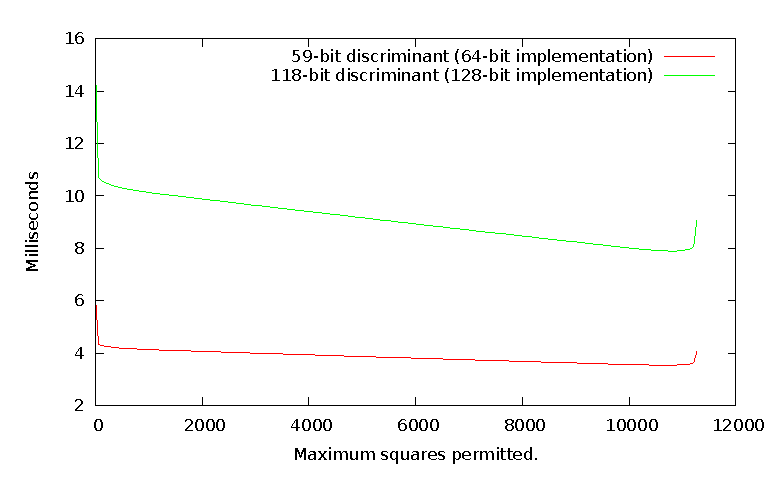
\includegraphics{dbns_l2r_vary_max}
\caption{The cost to exponentiate the $1000^{\textrm{th}}$ primorial, $n$, while varying the maximum number of squares permitted, $A$. The maximum number of cubes is $B = \ceil{\log_3(n/2^A)}$.}
\label{fig:dbnsL2rVaryBounds}
\end{figure}

In general, bounding the maximum number of squares and cubes give representations that lead to faster exponentiation in the ideal class group than representations where the number of squares or cubes is left unbound.  For this particular exponent, a representation generated without a global bound takes approximately 7.3 milliseconds for a 59-bit discriminant and 17.2 milliseconds for a 118-bit discriminant.  This is slower than all bounded representations for both implementations.

\section{Greedy Pruned Trees}

A right-to-left 2,3 chain can be generated by repeatedly reducing the exponent by 2 and 3 and then either adding or subtracting 1 and repeating this process until the exponent is 1.  In the windowed variant, after reducing the exponent by 2 and 3, we had 12 residues modulo $2^2 3^2$ and this lead to $2^{12}$ different strategies for adding or subtracting 1 from the residue.

In Subsection \ref{subsec:pm1Tree}, we discussed a tree based method where a set of at most $L$ \emph{partial representations} are maintained (a partial representation can be written as $n = x + \sum s_i2^{a_i}3^{b_i}$).  At each iteration, the $x$ term from each partial representation generates two new elements $x-1$ and $x+1$.  After reducing each new element by powers of 2 and 3, only the $L$ smallest are kept.  More formally, an element $x$ generates new integral elements $(x \pm 1)/(2^c3^d)$.

Here we consider two variations to the approach of maintaining the $L$ best\footnote{We say that a partial representation is \emph{better} when the $x$ term is smaller, or if the $x$ terms are equal, when the cost of the 2,3 summation is less.} partial representations. The first variation we consider is to generate several new nodes with integer values of the form $(x \pm 2^a3^b)/(2^c3^d)$, while the second variation is to include two terms such that each node generates values of the form $(x \pm 2^a \pm 3^b) / (2^c 3^d)$.  Notice that the first variation includes the forms $(x \pm 1)/(2^c 3^d)$ and so tends to give representations no worse than the method suggested by Doche and Habsieger \cite{Doche2008} (covered in Subsection \ref{subsec:pm1Tree}).  The assumption is that by adjusting $x$ by more than just 1, we increase the likelihood of finding a multiple of a large $2^c3^d$ window.

\mygraphTwo{pm2a3b_vary_max-64}{pm2a3b_vary_max-128}{fig:pm2a3bVaryMax}{Performance of varying the bounds $a, b \le U$ on $(x \pm 2^a3^b)/(2^c3^d)$ when exponentiating by the primorial $P_{1000}$.}
For both variations, we bound $a$ and $b$ such that $0 \le a \le U$ and $0 \le b \le U$.  Figure \ref{fig:pm2a3bVaryMax} shows the average time to exponentiate by the $1000^{\textrm{th}}$ primorial as the bound $U$ increases (using the $k=4$ best partial representations).  As $U$ increases, computing representations using this approach quickly becomes intractable.  We found that for our purposes, $U=16$ is an acceptable trade off between the average time to exponentiate and the time to generate the 2,3 representation.


\section{The $L$ Best Approximations}

The approach of maintaining a set of the $L$ best partial representations of an exponent can be adapted to that of the left-to-right 2,3 representation from Subsections \ref{subsec:ltorChains} and \ref{sec:ltorChains2}.  For an integer $x$ we say that $2^a3^b$ is a best approximation of $|x|$ when $\left||x| - 2^a3^b \right|$ is minimal.  The algorithm for the left-to-right representation (Subsection \ref{subsec:ltorChains}) finds a best approximation for $x$ and then repeats on the positive difference. However, instead of only iterating on the best approximation, each value from the set of partial representations generates new values of the form $\left||x| - 2^a3^b\right|$ (being careful to record the sign of $x$), and the $L$ best partial representations are retained.  In this case, we iterate $b$ from $0 \le b \le B$ and let $a_1 = \floor{\log_2 (x/3^b)}$ and $a_2 = \ceil{\log_2 (x/3^b)}$ bounding both $a_1, a_2 \le A$.  Note that using $a_2 = a_1 + 1$ is sufficient since either $\ceil{\log_2 (x/3^b)} = \floor{\log_2 (x/3^b)}$ or $\ceil{\log_2 (x/3^b)} = \floor{\log_2 (x/3^b)} + 1$.  We then use $\left||x|-2^{a_1}3^b\right|$ and $\left||x|-2^{a_2}3^b\right|$ as candidates for the new set.  As before, iterating the bound on the number of squares and cubes varies the cost of the representations generated.  


\section{Additive 2,3 Chains}

Imbert and Philippe \cite{Imbert2010b} give a method (see Subsection \ref{subsec:shortAddChains}) to compute the shortest additive strictly chained 2,3 partition, suitable for smaller integers.  Such partitions do not permit subtraction and every term is strictly less than and divides all subsequent terms. They take the form
\[
	n = \sum_{i=0}^k 2^{a_i}3^{b_i}
\]
for $a_i, b_i \in \ZZgez$ where $2^{a_i}3^{b_i}$ divides $2^{a_j}3^{b_j}$ and $a_i < a_j$ and $b_i < b_j$ for all $i < j$.

For our purposes, we modified this algorithm to compute additive 2,3 chains that minimize the average cost of arithmetic in the ideal class group -- the resulting additive 2,3 chains give a better average time for exponentiation, while they are not necessarily the shortest possible.  

Let $M$, $S$, and $C$ be the average cost to multiply, square, and cube respectively. Our modified function is as follows
\begin{equation*}
s'(n) = \begin{cases}
	\min\{S + s'(n/2), C + s'(n/3)\} & \textrm{when } n \equiv 0 \pmod 6 \\
	M + s'(n-1) & \textrm{when } n \equiv 1 \pmod 6 \\
	S + s'(n/2) & \textrm{when } n \equiv 2 \pmod 6 \\
	\min\{C + s'(n/3), M + S + s'((n-1)/2)\} & \textrm{when } n \equiv 3 \pmod 6 \\
	\min\{S + s'(n/2), M + C + s'((n-1)/3)\} & \textrm{when } n \equiv 4 \pmod 6 \\
	M + S + s'((n-1)/2) & \textrm{when } n \equiv 5 \pmod 6
\end{cases}
\end{equation*}
where $s'(1) = 0$, $s'(2) = S$, and $s'(3) = C$ are the base cases.

We also experimented with computing 2,3 strictly chained partitions that allow for both positive and negative terms.  The corresponding function we used is
\begin{equation*}
f(n) = \begin{cases}
	\min\{S + f(n/2), C + f(n/3)\} & \textrm{when } n \equiv 0 \pmod 6 \\
	\min\{M + f(n-1), M + S + f((n+1)/2)\} & \textrm{when } n \equiv 1 \pmod 6 \\
	\min\{S + f(n/2), M + C + f((n+1)/3)\} & \textrm{when } n \equiv 2 \pmod 6 \\
	\begin{split}\min\{C + f(n/3), M + S + f((n-1)/2),\\M + S + f((n+1)/2)\}\end{split} & \textrm{when } n \equiv 3 \pmod 6 \\
	\min\{S + f(n/2), M + C + f((n-1)/3)\} & \textrm{when } n \equiv 4 \pmod 6 \\
	\min\{M + f(n+1), M + S + f((n-1)/2)\} & \textrm{when } n \equiv 5 \pmod 6 \\
\end{cases}
\end{equation*}
again, where $f(1) = 0$, $f(2) = S$, and $f(3) = C$ are the base cases.  One thing to notice is that the function $s'$ computes a subset of the representations computed by the function $f$.  As such, we expect the average cost to exponentiate using a representation computed by $f$ to be no worse than the average cost to exponentiate using a representation computed by $s$.

\section{Incremental Searching}

For small inputs, the number of additive 2,3 chains is sufficiently reduced that we can compute all such chains in order to find the fastest.  Here we consider a different approach to searching for representations -- for a function generating a set of representations, we record the cheapest representation for each integer represented by the set.

We first iterate over all single term representations $2^{a_1}3^{b_1}$ for $0 \le a_1 \le A$ and $0 \le b_1 \le B$, and then all two term representations $2^{a_1}3^{b_1} \pm 2^{a_2}3^{b_2}$ for $0 \le a_1 < a_2 \le A$ and $0 \le b_1 < b_2 \le B$.  In general, we compute the set of representations
\[
R = R_1 \cup R_2 \cup ... \cup R_m
\]
for some maximum number of terms $m$ where
\[
R_k = \left\{\sum_{i=1}^k\pm 2^{a_i}3^{b_i} ~:~ 0 \le a_1 < \cdots < a_k \le A \textrm{ and } 0 \le b_1 < \cdots < b_k \le B \right\}.
\]
We iterate over the set $R$ and for each integer represented, we record the lowest cost representation for that integer in $R$.

In our experiments, we search for representations for 16-bit integers. We intially chose $A = \ceil{\log_2\left(2^{16}\right)} = 16$, $B = \ceil{\log_3 \left(2^{16}\right)} = 11$, and iterated the number of terms $k$ from 1 through 5. For representations of $k = 6$ terms, our implementation did not complete after a week of execution.  We then ran our search again using $A=18$ and $B=12$ and found that none of our minimal representations were improved.

Since both the incremental search of this Subsection and the two functions from the previous Subsection are computationally expensive, we are only able to compute chains for small exponents.  This is still useful when we consider methods that partition large exponents into smaller blocks using their binary representation, or when we consider multiple exponentiations by a list of prime powers.


\subsection{Big Exponents from Small Exponents}

The techniques of the previous two Subsections are computationally expensive and as such, we limit our search to representations of 16-bit integers.  One way that we use such representations is to write the exponent $n$ in 16-bit blocks as
\[
	n = \sum_{i=0}^k 2^{16i} b_i
\]
where $0 \le b_i < 2^{16}$.  Assuming that we can exponentiate a group element $g$ to a 16-bit exponent $b_i$, Algorithm \ref{alg:blockedExp} computes the exponentiation $g^n$ using an approach similar to a left-to-right windowed binary exponentiation.

\begin{algorithm}[H]
\caption{16-bit Blocked Exponentiation.}
\label{alg:blockedExp}
\begin{algorithmic}[1]
\REQUIRE $n \in \ZZ, g \in G$ and a method to compute $g^{b_i}$ for $0 \le b_i < 2^{16}$.
\ENSURE $g^n$.
\STATE $R \gets 1_G$
\FOR {$i$ from $\ceil{\log_{2^{16}} n}$ downto 0}
	\STATE $R \gets R^{2^{16}}$ \COMMENT{By repeated squaring.}
	\STATE $b_i \gets \floor{n / 2^{16i}} \bmod {2^{16}}$
	\STATE $R \gets R \cdot g^{b_i}$
\ENDFOR
\RETURN $R$
\end{algorithmic}
\end{algorithm}

Another way we can use 16-bit representations is when we know the prime factorization of the exponent $n$ and $n$ is the product of primes smaller than $2^{16}$.  Since we are interested in exponentiation by primorials (i.e.\ the product of the first $w$ primes), the prime factorization is trivial. Given a primorial $P_w = \prod_{i=1}^w p_i$ where $p_i$ is the $i^{\textrm{th}}$ prime, we can compute $g^{P_w}$ as $(((g^{p_1})^{p_2})^{\cdots})^{p_w}$ using a series of $w$ small exponentiations.

\subsection{Experimental Results}

One reason to improve the performance of exponentiation in the ideal class group is to improve the performance of order finding in this group.  In particular, we exponentiate a random ideal class to a primorial so that the order of the resulting ideal class is likely to be coprime to our exponent.

Two of the techniques in the previous section compute $g^n$ using a series of smaller exponentiations $g^b$ such that $0 \le b < 2^{16}$.  So we begin by determining the best method to exponentiate using 16-bit exponents.  To do so, we compute the average time to exponentiate for exponents 1 through 65535 using 59-bit and 118-bit discriminants.  Table \ref{tab:exp16bitWinners} shows the number of exponents for which each method was the fastest\footnote{The methods not listed in this table were not the fastest for any exponents.}.
\begin{table}[h]
\centering
\begin{tabular}{| l | r | r |}
	\hline
	Method & 59-bit Discriminants & 118-bit Discriminants \\
	\hline
	Left-to-Right 2,3 Representation & 2536 & 7097 \\
	4 Best $\left||x|-2^a3^b\right|$ & 9091 & 7230 \\
	4 Best $(x \pm 2^a3^b)/(2^c3^d)$ & 47969 & 45468 \\
	4 Best $(x \pm 2^a \pm 3^b)/(2^c3^c)$ & 3333 & 2756 \\
	Recursive $\sum 2^a3^b$ Chains & 2406 & 2970 \\
	Incremental Search & 199 & 13 \\
	\hline
\end{tabular}
\caption{The number of exponents for which each method gave the fastest average time to exponentiate.}
\label{tab:exp16bitWinners}
\end{table}
For each exponent, we then normalized the time of each method relative to the best time.  Table \ref{tab:exp16bitTimes} shows the average of these normalized times.
\begin{table}[h]
\centering
\begin{tabular}{| l | c | c |}
	\hline
	Method & 59-bit Discriminants & 118-bit Discriminants \\
	\hline
	Binary & 1.48864 & 1.44287 \\
	Right-to-Left Non-Adjacent Form & 1.39605 & 1.34547 \\
	Right-to-Left 2,3 Chain & 1.35869 & 1.37595 \\
	$2^2 3^2$ Windowed Right-to-Left 2,3 Chain & 1.38676 & 1.37415 \\
	Left-to-Right 2,3 Representation & 1.27775 & 1.23781 \\
	4 Best $\left||x|-2^a3^b\right|$ & 1.19508 & 1.17034 \\
	4 Best $(x \pm 1)/(2^c3^d)$ & 1.23152 & 1.22800 \\
	4 Best $(x \pm 2^a3^b)/(2^c3^d)$ & 1.03227 & 1.03886 \\
	4 Best $(x \pm 2^a \pm 3^b)/(2^c3^c)$ & 1.37963 & 1.38966 \\
	Recursive $\sum 2^a3^b$ Chains & 1.28606 & 1.26822 \\
	Recursive $\sum \pm 2^a3^b$ Chains & 1.21295 & 1.18712 \\
	Incremental Search & 1.19495 & 1.17059 \\
	\hline
\end{tabular}
\caption{The normalized time to exponentiation relative to the fastest time for each exponent.}
\label{tab:exp16bitTimes}
\end{table}
The method that maintains the 4 best partial representations of the form $(x \pm 2^a3^b)/(2^c3^d)$ was the best performer in general.  However, since we were interested in precomputing 16-bit representations for use with a block exponentiation and exponentiation by a list of prime factors, we used the best representation available for each exponent.

To determine the best method to exponentiate a random ideal by a primorial, we compute the average time to exponentiate for the primorials $P_{250k}$ for $1 \le k \le 100$.  We categorized the different exponentiation techniques as those that use only base 2, those that generate 2,3 chains from right-to-left, from left-to-right, that add or subtract to a partial representation and then reduce by $2^c3^d$, and those that make use of the best 16-bit representations.  We then compared the average time to exponentiate each method from a category, and finally compared the best performers of each category to determine the best performer overall.

We found that for both our 64-bit and 128-bit implementations and for all primorials tested, the method of iterating on the 4 best $\left||x| - 2^a3^b\right|$ approximations leads to representations with the fastest time to exponentiate.  This is in contrast to the method of iterating on the 4 best partial representations $(x \pm 2^a3^b)/(2^c3^d)$ that lead to the best timings for 16-bit integers.  Naturally, we can improve these results by iterating on the $L$ best partial representations for $L > 4$ at the expense of longer precomputation.

Figures \ref{fig:expBinNaf64} and \ref{fig:expBinNaf128} compare binary exponentiation against right-to-left non-adjacent form representation.  The non-adjacent form representation leads to faster exponentiations in all cases.  Figures \ref{fig:expDbnsR2L64} and \ref{fig:expDbnsR2L128} compare the non-windowed right-to-left 2,3 chain method to the $2^2 3^2$ windowed method.  The $2^23^2$ windowed method out performs the non-windowed method for all exponents.  Figures \ref{fig:expDbnsL2R64} and \ref{fig:expDbnsL2R128} compare left-to-right 2,3 representations with that of maintaining the 4 best $\left||x|-2^a3^b\right|$ approximations.  In this case, maintaining the 4 best approximations performs best.  Figures \ref{fig:expPmVariants64} and \ref{fig:expPmVariants128} compare the three different techniques of adding or subtracting a value to a partial representation and then reducing by a power of 2 and 3.  Here, computing candidates $(x-2^a3^b)/(2^c3^d)$ leads to representations that exponentiate the fastest.  Figures \ref{fig:expBlockList64} and \ref{fig:expBlockList128} compare the two methods that rely on the best found 16-bit representations.  In this case, when the factorization of the exponent is easily known, it is faster to exponentiation by the list of prime factors than it is to represent the exponent using 16-bit blocks.  Finally, Figures \ref{fig:expWinners64} and \ref{fig:expWinners128} compare the best performer from each category.

\mygraph{binary_vs_naf-64}{fig:expBinNaf64}{Base 2 Exponentiation (59-bit Discriminants).}
\mygraph{binary_vs_naf-128}{fig:expBinNaf128}{Base 2 Exponentiation (118-bit Discriminants).}

\mygraph{dbns_r2ls-64}{fig:expDbnsR2L64}{Right-to-Left 2,3 Chains (59-bit Discriminants).}
\mygraph{dbns_r2ls-128}{fig:expDbnsR2L128}{Right-to-Left 2,3 Chains (118-bit Discriminants).}

\mygraphTwo{dbns_l2rs-64}{dbns_l2rs-64-zoom}{fig:expDbnsL2R64}{Left-to-Right 2,3 Representations (59-bit Discriminants).}
\mygraphTwo{dbns_l2rs-128}{dbns_l2rs-128-zoom}{fig:expDbnsL2R128}{Left-to-Right 2,3 Representations (118-bit Discriminants).}

\mygraphTwo{pm_variants-64}{pm_variants-64-zoom}{fig:expPmVariants64}{4 Best $(x\pm\cdots)/(2^c3^d)$ (59-bit Discriminants).}
\mygraphTwo{pm_variants-128}{pm_variants-128-zoom}{fig:expPmVariants128}{4 Best $(x\pm\cdots)/(2^c3^d)$ (118-bit Discriminants).}

\mygraph{block_vs_list-64}{fig:expBlockList64}{Use $g^b$ for 16-bit $b$ (59-bit Discriminants).}
\mygraph{block_vs_list-128}{fig:expBlockList128}{Use $g^b$ for 16-bit $b$ (118-bit Discriminants).}

\mygraph{winners-64}{fig:expWinners64}{The best performers from each category (59-bit Discriminants).}
\mygraph{winners-128}{fig:expWinners128}{The best performers from each category (118-bit Discriminants).}


\section{Summary}

This Chapter presented the approach and results used to improve exponentiation in the ideal class group of imaginary quadratic number fields.  Several methods for exponentiation including novel extensions to methods for computing 2,3 chains and representations were explored.  We found that for 16-bit exponents, the method of iterating on the $L$ best partial representations $x + \sum s_i2^{a_i}3^{b_i}$ such that each $x$ generates new terms of the form $(x \pm 2^a 3^b)/(2^c3^d) \in \ZZ$ gives the fastest representation on average.  For large primorial exponents, generating new terms of the form $\left||x|-2^a3^b\right|$ gave the fastest representations on average.

The next Chapter brings together the improvements to ideal arithmetic and exponentiation in our implementation of SuperSPAR -- an algorithm with the fastest average time to factor integers $n$ in the range $2^{54} \le n < 2^{63}$ of the integer factoring algorithms that we tested.



%%%%%%%%%%%%%%%%%%%%%%%%%
% CHAPTER 7             %
% SUPERSPAR EXPERIMENTS %
%%%%%%%%%%%%%%%%%%%%%%%%%
\chapter{SuperSPAR Experiments}
\label{chap:ssparExperiments}

\section{Motivation: How fast can we make SuperSPAR}

\section{Coprime Finding}
\begin{itemize}
\item Wheeling
\item Sieving
\item Delta Tables
\end{itemize}

\section{Exponentiation}
\label{sec:ssparExp}
\subsection{Bounds for primorial (bound for prime vs exponent)}
\subsection{Primorial vs Prime Powers}
i.e. is it faster to use the product and one exponentiation or individual primes and many exponentations

machine representation of 2,3 representation for primorials

\subsection{Best primorial bound for n-bit integers}

\section{Time Spent on Exponentiation vs. Search}
\label{sec:ssparExpVsSearch}

Let $s$ be a function from some multiple $m$ of the primorial $P_w$ to the total number of baby steps and giant steps taken during the search stage of the algorithm.  We have
\[
	s(m, w) = 2 m \phi(P_w).
\]
Then, let
\[
	g(m, w) = 2 m^2 \phi(P_w) P_w
\]
be a function that computes the exponent of the final giant step before the algorithm tries a different multiplier.  In general, if there exists some $m'$ and $w'$ such that 
\[
g(m', w') > g(m, w) \textrm{ and } s(m', w') \le s(m, w)
\]
this means that by choosing a multiple $m'$ of the primorial $P_{w'}$, the search phase can search further using the same or fewer steps.  Let $S$ be the set of pairs $(m, w)$ from which we select the bound $b$ on the baby steps
\[
  S = \left\{ (m, w) ~:~ g(m, w) > g(m', w') \textrm{ for all }  \right\}
\]


\section{Sequential prime ideals vs random prime ideals}

\section{Ratio of prime ideals to multipliers}
\label{sec:ssparIdealsToMultipliers}

\section{Best multipliers to use}

\section{Chained Hashing vs Open Address Hashing}

Only hash the pair $(a,c)$ so that $\aclass$ and $\aclass^{-1}$ hash to the same value.

\section{Empirical search for primorial and step count}
\begin{itemize}
\item Linear, grid, 2d quadratic, 1d grid + binary search on step count.
\item (Quadratic samples at 1/3 and 2/3 and throws away the larger third)
\end{itemize}

\section{Comparison with other algorithms}
\begin{itemize}
\item Pari/GP
\item Custom SQUFOF
\item GNU MSieve
\item GNU-ECM
\item YAFU
\item Flint
\item Maple
\end{itemize}


%%%%%%%%%%%%%%%%%%%%
% CHAPTER 8        %
% FURTHER RESEARCH %
%%%%%%%%%%%%%%%%%%%%
\chapter{Further Research}

\subsection{Improvements}

Time 2,3 representation generation vs 2,3 exponentiation.
A rigorous analysis of the expected cost of each 2,3 representation generated.

Windowed left-to-right GCD.
2,3 base GCD.

Inclusion into supervisor's ANTL library and hopefully Sage or/and Pari/GP.

Try some extremely large (1Gb+) primorials that are written to disk, powering 2,3 r2l chain of them, and then doing a pollard-rho or something with a smaller primorial for the same number of steps.  The idea being to simulate the original SPAR, but with our library and a few dbns tricks.  Then we try factoring some much larger composites.

This might be interesting to try a discrete log record too.

Large differences in exponents show general trends to 2,3 representations, however, when we look close up, the variation in 2, 3 representations between $n$ and $n+1$ varies greatly.  It might be interesting to measure how much they vary.  


\section{Other types of Ideal Arithmetic}
For example, the ideal ring of algebraic integers of real quadratic fields.

\section{Function Fields}

For example Hyperelliptic Curves

\section{DBNS with other coprime bases}

Could try tree based approaches where we approximate the cost of the complete chain based on the partial chain, rather than using the smallest remaining exponent and the cost to break ties.

\section{Number systems with three, four, or more bases.}

\section{$\textrm{Super}^2\textrm{SPAR}$}

SuperSPAR with other corprime bases or multiple bases.

In our implementation we choose a primorial, $P$, such that baby steps are coprime to $P$ and giant steps are a multiple of $P$.  We can select a product of small primes that need not be consecutive, e.g. $P = 2 \times 3 \times 11 \times 13$ and then use baby steps coprime to this and giant steps that are a multiple of this.

Also consider parallelization of SuperSPAR using multipliers.  And possibly implementing it on a GPU.

Median time to factor. 5-number summary graph might be interesting: \url{http://en.wikipedia.org/wiki/Five-number_summary}. Top 10\%.  That kind of thing.

More rigorous analysis of the median running time, etc.

%%%%%%%%%%%%%%%%
% BIBLIOGRAPHY %
%%%%%%%%%%%%%%%%
\bibliographystyle{plain}
\bibliography{Bibliography}


\end{document}
